\section{Experiments}

In this section, we are going to run the \textbf{Analyser} pipeline which consists of two steps: simple and complex analysis. All experiments have been run on a MacBook Pro (Retina, 13-inch, Early 2015) (See Table \ref{tab: mac spec}). 

\begin{table}[h!]
    \centering
    \begin{tabular}{|c|c|}
         \hline
         \textbf{Name} & \textbf{Value} \\
         \hline
         Model & MacBook Pro (Retina, 13-inch, Early 2015) \\
         \hline
         GPU & Intel Iris Graphics 6100 1536 MB \\
         \hline
         CPU & 2.7 GHz Intel Core i5 \\
         \hline
         RAM & 8 GB 1867 MHz DDR3 \\
         \hline
         Disk & 256 GB (SSD) \\
         \hline
    \end{tabular}
    \caption{Mac Book Pro specifications}
    \label{tab: mac spec}
\end{table}

The LSTM Bagging Planner defines custom statistic measures described in Table \ref{tab: LSTM Bagging Planner testing_tab}.

\begin{table}[h!]
    \centerfloat
    \begin{tabular}{|c|c|M{8cm}|}
         \hline
         \textbf{Name} & \textbf{Supported Algorithms} & \textbf{Description} \\
         \hline
         Kernels & \texttt{LSTM Bagging Planner} & The name of all kernels in priority order \\
         \hline
         Pick Ratio & \texttt{LSTM Bagging Planner} & The "best behaving" kernel picked by the algorithm \\
         \hline
    \end{tabular}
    \caption{LSTM Bagging Planner statistic measure}
    \label{tab: LSTM Bagging Planner testing_tab}
\end{table}

The Global Way-point LSTM Planner defines custom display information (See Table \ref{tab: WayPointNavigation map_dsiplays}) and custom statistic measures (See Table \ref{tab: WayPointNavigation testing_tab}).

\begin{table}[h!]
    \centerfloat
    \begin{tabular}{|M{2cm}|M{2.7cm}|M{9cm}|}
         \hline
         \textbf{Display Name} & \textbf{Supported Algorithms} & \textbf{Description} \\
         \hline
         Way-points & \texttt{Global Way-point LSTM Planner} & Displays the global kernel suggested way-points with cyan squares/circles (depending if the map is displayed as a grid or not) \\
         \hline
         Total Search Space & \texttt{Global Way-point LSTM Planner} & Displays the Total Search Space of the local kernel as dark-grey entities (local kernel has to be from A* family) \\
         \hline
    \end{tabular}
    \caption{Global Way-point LSTM Planner information displays}
    \label{tab: WayPointNavigation map_dsiplays}
\end{table}

\begin{table}[h!]
    \centerfloat
    \begin{tabular}{|M{2.7cm}|M{2.7cm}|M{8cm}|}
         \hline
         \textbf{Name} & \textbf{Supported Algorithms} & \textbf{Description} \\
         \hline
         GK Improvement & \texttt{Global Way-point LSTM Planner} & How much did the global kernel contributed to the final path. It is the local kernel travelled distance from the first way-point to the last way-point as a percentage from the total travelled distance \\
         \hline
         GK Steps & \texttt{Global Way-point LSTM Planner} & The total steps (movements) taken by the local kernel from the first way-point to the last way-point \\
         \hline
         GK Distance & \texttt{Global Way-point LSTM Planner} & The total local kernel travelled distance from the first way-point to the last way-point \\
         \hline
         GK Distance Left & \texttt{Global Way-point LSTM Planner} & The Euclidean distance between the last way-point and the goal  \\
         \hline
         GK Calls & \texttt{Global Way-point LSTM Planner} & The number of global kernel calls \\
         \hline
         WP & \texttt{Global Way-point LSTM Planner} & The number of suggested way-points (we use this over the GK Calls as they are correlated) \\
         \hline
         WP In-Between Distance & \texttt{Global Way-point LSTM Planner} & The average Euclidean distance between way-points \\
         \hline
         Pick Ratio & \texttt{Global Way-point LSTM Planner} & The kernel pick percentages from the global kernel (global kernel has to be an LSTM Bagging Planner) \\
         \hline
         Search Space & \texttt{Global Way-point LSTM Planner} & The search space (visited set) that was used to find the path (without priority queue) (local kernel has to be from A* family) \\
         \hline
         Total Fringe & \texttt{Global Way-point LSTM Planner} & The left priority queue size, after the goal was found (local kernel has to be from A* family) \\
         \hline
         Total Search & \texttt{Global Way-point LSTM Planner} & Total Search = Search Space + Total Fringe (local kernel has to be from A* family) \\
         \hline
         Session Search Space & \texttt{Global Way-point LSTM Planner} & The average session search space (visited set) that was used to find the path (without priority queue) (local kernel has to be from A* family) \\
         \hline
         Session Fringe & \texttt{Global Way-point LSTM Planner} & The average session left priority queue size, after the goal was found (local kernel has to be from A* family) \\
         \hline
         Session Search & \texttt{Global Way-point LSTM Planner} & Session Search = Session Search Space + Session Fringe (local kernel has to be from A* family) \\
         \hline
    \end{tabular}
    \caption{Global Way-point LSTM Planner statistic measures}
    \label{tab: WayPointNavigation testing_tab}
\end{table}

\FloatBarrier

While analysing the algorithms, we will make use of the statistic measures defined in Tables \ref{tab: a_testing_tab}, \ref{tab: LSTM Bagging Planner testing_tab} and \ref{tab: WayPointNavigation testing_tab}. 

%For convenience we have provided a pruned table which contains all used statistical measures (See table \ref{tab: eval_stats}).

%\begin{table}[h!] 
%\centerfloat
%\begin{tabular}{|M{2.2cm}|M{3.3cm}|M{8cm}|}
%\hline
%         \textbf{Name} & \textbf{Supported %Algorithms} & \textbf{Description} \\
%         \hline
%         Map Obstacle Ratio & \texttt{All} & The %percentage of obstacles from the map \\
%         \hline
%         Original Distance & \texttt{All} & The %euclidean distance from agent to goal at %the beginning of the algorithm \\
%         \hline
%         Algorithm Type & \texttt{All} & The type of %the algorithm that was run \\
%         \hline
%         Success Rate & \texttt{All} & The rate of %success of finding a path from the agent to %the goal \\
%         \hline
%         Distance & \texttt{All} & The total %distance taken to reach the goal. Steps is %different from Distance as diagonal step is %considered 1, but diagonal distance is %considered $\sqrt{2}$ \\
%         \hline
%         Time & \texttt{All} & The total time taken to reach the goal \\
%         \hline
%         Distance Left & \texttt{All} & In case of %failure what is the euclidean distance left %from agent to goal \\
%         \hline
%         GK Improvement & \texttt{Way-Point %Navigation Planner} & How much did the %global kernel contributed to the final %path. It is the travelled distance by the %local kernel from the first way-point to %the last way-point as a percentage from the %total travelled distance \\
%         \hline
%         GK Distance & \texttt{Global Way-point LSTM Planner %Planner} & The total local kernel travelled %distance from the first way-point to the %last way-point \\
%         \hline
%         GK Distance Left & \texttt{Way-Point %Navigation Planner} & The euclidean %distance between the last way-point and the %goal  \\
%         \hline
%         WP & \texttt{Global Way-point LSTM Planner} %& The number of suggested way-points (we use this over the GK Calls as they are correlated) \\
%         \hline
%         WP In-Between Distance & \texttt{Way-Point %Navigation Planner} & The average euclidean %distance between way-points \\
%         \hline
%         Kernels & \texttt{LSTM Bagging Planner}, %\texttt{Global Way-point LSTM Planner} & The %name of all kernels from the global kernel %(global kernel has to be an LSTM Bagging %Planner) \\
%         \hline
%         Pick Ratio & \texttt{Global Way-point LSTM Planner %Planner} & The kernel pick percentages from %the global kernel (global kernel has to be %an LSTM Bagging Planner) \\
%         \hline
%         Fringe & \texttt{Global Way-point LSTM Planner %Planner} & The left priority queue size, %after the goal was found (local kernel has %to be from A* family) \\
%         \hline
%         Total Search & \texttt{Global Way-point LSTM Planner %Planner} & Total Search Space = Search %Space + Fringe (local kernel has to be from %A* family) \\
%         \hline
%         Session Fringe & \texttt{A*}, %\texttt{Dijkstra}, \texttt{Way-Point %Navigation Planner} & The average session %left priority queue size, after the goal %was found (local kernel has to be from A* %family) \\
%         \hline
%         Session Total Search & \texttt{A*}, %\texttt{Dijkstra}, \texttt{Way-Point %Navigation Planner} & Session Total Search %= Session Search Space + Session Fringe %(local kernel has to be from A* family) \\
%         \hline
%    \end{tabular}
%\caption{\textbf{Used} evaluation statistic metrics}
%\label{tab: eval_stats} 
%\end{table}

For each routine, we are going to produce four tables similar to Table \ref{tab: eval_simple_analysis}. The first table describes the general performance of all algorithms compared to A* (Algorithm \hyperref[tab: evalalgorithms]{0}). It should be mentioned that the time statistics for the LSTM Bagging Planner (Algorithm \hyperref[tab: evalalgorithms]{11}) and the proposed solution (Algorithm \hyperref[tab: evalalgorithms]{14}) are significantly higher due to the parallelism issue (algorithms were run sequentially). The second table refers to the pick percentages of the internal kernels (See Table \ref{tab: eval_lstm_bagging} for kernel reference) of the LSTM Bagging Planner (Algorithm \hyperref[tab: evalalgorithms]{11}) and the proposed solution (Algorithm \hyperref[tab: evalalgorithms]{14})  and is used to check the kernel pick distribution. The third table is associated with the Global Way-point LSTM Planner algorithms only and displays statistics which showcase the global kernel efficiency. For instance, if the WP In-Between Distance is higher, than we are more confident that the global kernel has proposed more efficient way-points. The final table displays the used memory space of the local kernel. We use four statistics: Total Search (the total local kernel memory (including fringe)), Total Fringe (the total local kernel fringe space), Session Search (the average local kernel session exploration (including fringe)) and Session Fringe (the average local kernel session fringe space).

The simple analysis stage is run on 30 maps (10 of each type) and the results are averaged (See Table \ref{tab: eval_simple_analysis}). The complex analysis stage is run on 6 maps (3 generated and 3 hand crafted; See Figures \ref{fig: rep_Uniform Random Fill Map}, \ref{fig: rep_Block Map}, \ref{fig: rep_House Map}, \ref{fig: rep_Hand Crafted Map 1}, \ref{fig: rep_Hand Crafted Map 2} and \ref{fig: rep_Hand Crafted Map 3}). For each map we sample 50 random positions (agent and goal) and average the results of all 50 runs. At the end the overall results are reported in Table \ref{tab: eval_complex_analysis_overall}.

As a frame of reference the comprehensive results from \cite{nicola2018lstm} are shown in Table \ref{tab: nicola_results}. The authors from \cite{nicola2018lstm} state that they have used 50 equally selected paths from 10 different maps for each environment type when evaluating their proposed solution. The authors from \cite{inoue2019robot} state that they have achieved over 98\% in 8 out of 10 environment maps. Moreover, the authors from \cite{inoue2019robot} state that the generalisation property to unknown environments has been checked and confirmed. The results showed that the planner from \cite{inoue2019robot} still has a high success rate in unknown maps, but path generation fails under environments which are significantly different from the trained environments. It should be mentioned that \cite{inoue2019robot} associates a fail with a path that has found the goal, but overlaps obstacles. This is because their solution is offline and the network returns the full generated path, which consequently might collide with other obstacles. Therefore, the path generation fail under unknown environments does not theoretically contradict the robustness to unknown environments (since a path to the goal has been found). However, we should emphasise that our evaluation methods and results refer only to completely successful paths (i.e. collision-free trajectories). Lastly, the authors from \cite{nicola2018lstm} use the same collision-free evaluation constraint and therefore, we can relate and make comparisons against their results.

\begin{table}[h!]
    \centerfloat
    \begin{tabular}{|M{1.4cm}|M{2.3cm}|M{1.3cm}|M{1.3cm}|c|M{1.8cm}|M{1.7cm}|}
       \hline
       \textbf{Planner} & \textbf{Maps} & \textbf{Nr. of Paths} & \textbf{Nr. of Maps} & \textbf{Success Rate} & \textbf{Average Time (s)} & \textbf{Average Length} \\
       \hline
       A* & Dragon Age & 50 & 10 & 100\% & $3.37 \cdot 10^{-4}$ & 45.82 \\
       \hline
       Online LSTM & Dragon Age & 50 & 10 & 68\% (I: -32\%) & $1.69 \cdot 10^{-3}$ & 53.39 (I:-16.52\%) \\
       \hline
       A* & Mazes with corridor 8 steps long & 50 & 10 & 100\% & $2.96 \cdot 10^{-4}$ & 50.90\\
       \hline
       Online LSTM & Mazes with corridor 8 steps long & 50 & 10 & 26\% (I: -74\%) & $1.98 \cdot 10^{-3}$ & 61.71 (-21.24\%) \\
       \hline
       A* & Random filled & 50 & 10 & 100\% & $2.84 \cdot 10^{-4}$ & 61.60 \\
       \hline
       Online LSTM & Random filled & 50 & 10 & 82\% (I: -18\%) & $2.04 \cdot 10^{-3}$ & 71.60 (I: -16.23\%) \\
       \hline
    \end{tabular}
    \caption{\cite{nicola2018lstm} results (50 paths selected equally from 10 different maps for each environment type). The parenthesis value with prefix I: is the improvement rate against A*}
    \label{tab: nicola_results}
\end{table}

\pagebreak

\pagebreak

\begin{table}[] 
\footnotesize 
\small
\centering

\begin{tabular}{|cc|c|c|c|c|c|}
\hline
\multicolumn{2}{|c|}{\textbf{Nr.}} & \textbf{Success Rate} & \textbf{Distance} & \textbf{Time} & \textbf{Distance Left}\\
\hline
\hline
\multicolumn{2}{|c|}{\cellcolor{lightgray!20} \hyperref[tab: evalalgorithms]{0}} & 93.33\% (I: 0\%) & 39.55 (A*: 39.55) (I: 0\%) & 0.055s & 2.36\\
\hline
\hline
\multicolumn{2}{|c|}{\cellcolor{red!40} \hyperref[tab: evalalgorithms]{1}} & 46.67\% (I: -49.99\%) & 35.09 (A*: 34.06) (I: -3.02\%) & 0.1342s & 9.93\\
\hline
\multicolumn{2}{|c|}{\cellcolor{red!20} \hyperref[tab: evalalgorithms]{2}} & 46.67\% (I: -49.99\%) & 44.04 (A*: 36.77) (I: -19.77\%) & 0.1728s & 12.52\\
\hline
\multicolumn{2}{|c|}{\cellcolor{red!20} \hyperref[tab: evalalgorithms]{3}} & 60.0\% (I: -35.71\%) & 45.44 (A*: 38.97) (I: -16.6\%) & 0.1328s & 6.29\\
\hline
\multicolumn{2}{|c|}{\cellcolor{red!20} \hyperref[tab: evalalgorithms]{4}} & 50.0\% (I: -46.43\%) & 37.43 (A*: 35.07) (I: -6.73\%) & 0.1051s & 9.45\\
\hline
\multicolumn{2}{|c|}{\cellcolor{red!20} \hyperref[tab: evalalgorithms]{5}} & 70.0\% (I: -25.0\%) & 43.88 (A*: 38.59) (I: -13.71\%) & 0.1166s & 6.47\\
\hline
\hline
\multicolumn{2}{|c|}{\cellcolor{blue!20} \hyperref[tab: evalalgorithms]{6}} & 40.0\% (I: -57.14\%) & 28.15 (A*: 27.14) (I: -3.72\%) & 0.1047s & 14.24\\
\hline
\multicolumn{2}{|c|}{\cellcolor{blue!40} \hyperref[tab: evalalgorithms]{7}} & 43.33\% (I: -53.57\%) & 37.96 (A*: 33.79) (I: -12.34\%) & 0.1399s & 13.59\\
\hline
\multicolumn{2}{|c|}{\cellcolor{blue!20} \hyperref[tab: evalalgorithms]{8}} & 56.67\% (I: -39.28\%) & 44.16 (A*: 39.03) (I: -13.14\%) & 0.1579s & 10.52\\
\hline
\multicolumn{2}{|c|}{\cellcolor{blue!20} \hyperref[tab: evalalgorithms]{9}} & 56.67\% (I: -39.28\%) & 42.19 (A*: 36.86) (I: -14.46\%) & 0.1513s & 7.68\\
\hline
\multicolumn{2}{|c|}{\cellcolor{blue!20} \hyperref[tab: evalalgorithms]{10}} & 60.0\% (I: -35.71\%) & 40.58 (A*: 36.29) (I: -11.82\%) & 0.1452s & 7.38\\
\hline
\hline
\multicolumn{2}{|c|}{\cellcolor{orange!40} \hyperref[tab: evalalgorithms]{11}} & 83.33\% (I: -10.71\%) & 43.22 (A*: 40.33) (I: -7.17\%) & 1.3548s & 1.63\\
\hline
\hline
\multicolumn{1}{|M{0.15cm}}{\cellcolor{cyan!40}} & \multicolumn{1}{M{0.15cm}|}{\cellcolor{blue!40} \hspace*{-0.5cm}\hyperref[tab: evalalgorithms]{12}} & 93.33\% (I: 0\%) & 45.76 (A*: 39.55) (I: -15.7\%) & 0.407s & 0.95\\
\hline
\multicolumn{1}{|M{0.15cm}}{\cellcolor{cyan!40}} & \multicolumn{1}{M{0.15cm}|}{\cellcolor{red!40} \hspace*{-0.5cm}\hyperref[tab: evalalgorithms]{13}} & 93.33\% (I: 0\%) & 48.95 (A*: 39.55) (I: -23.77\%) & 0.3171s & 0.62\\
\hline
\multicolumn{1}{|M{0.15cm}}{\cellcolor{cyan!40}} & \multicolumn{1}{M{0.15cm}|}{\cellcolor{orange!40} \hspace*{-0.5cm}\hyperref[tab: evalalgorithms]{14}} & 93.33\% (I: 0\%) & 44.94 (A*: 39.55) (I: -13.63\%) & 2.8274s & 0.64\\
\hline
\end{tabular}


\bigskip

\begin{tabular}{|cc|c|c|}
\hline
\multicolumn{2}{|c|}{\textbf{Nr.}} & \textbf{Pick Ratio}\\
\hline
\hline
\multicolumn{2}{|c|}{\cellcolor{orange!40} \hyperref[tab: evalalgorithms]{11}} & [23.33, 26.67, 10.0, 3.33, 3.33, 6.67, 10.0, 10.0, 0.0, 6.67]\%\\
\hline
\hline
\multicolumn{1}{|M{0.15cm}}{\cellcolor{cyan!40}} & \multicolumn{1}{M{0.15cm}|}{\cellcolor{orange!40} \hspace*{-0.5cm}\hyperref[tab: evalalgorithms]{14}} & [51.31, 21.02, 12.66, 3.43, 0.67, 0.0, 7.9, 1.67, 0.24, 1.11]\%\\
\hline
\end{tabular}


\bigskip

\begin{tabular}{|cc|c|c|c|c|M{3cm}|}
\hline
\multicolumn{2}{|c|}{\textbf{Nr.}} & \textbf{GK Improvement} & \textbf{GK Distance} & \textbf{GK Distance Left} & \textbf{WP} & \textbf{WP In-Between Distance}\\
\hline
\hline
\multicolumn{1}{|M{0.15cm}}{\cellcolor{cyan!40}} & \multicolumn{1}{M{0.15cm}|}{\cellcolor{blue!40} \hspace*{-0.5cm}\hyperref[tab: evalalgorithms]{12}} & 73.74\% & 30.97 & 11.08 & 5.03 & 10.12\\
\hline
\multicolumn{1}{|M{0.15cm}}{\cellcolor{cyan!40}} & \multicolumn{1}{M{0.15cm}|}{\cellcolor{red!40} \hspace*{-0.5cm}\hyperref[tab: evalalgorithms]{13}} & 86.51\% & 44.63 & 5.51 & 4.3 & 14.14\\
\hline
\multicolumn{1}{|M{0.15cm}}{\cellcolor{cyan!40}} & \multicolumn{1}{M{0.15cm}|}{\cellcolor{orange!40} \hspace*{-0.5cm}\hyperref[tab: evalalgorithms]{14}} & 97.0\% & 49.23 & 1.3 & 4.1 & 15.91\\
\hline
\end{tabular}


\bigskip

\begin{tabular}{|cc|c|c|c|c|c|}
\hline
\multicolumn{2}{|c|}{\textbf{Nr.}} & \textbf{Total Search} & \textbf{Total Fringe} & \textbf{Session Search} & \textbf{Session Fringe}\\
\hline
\hline
\multicolumn{2}{|c|}{\cellcolor{lightgray!20} \hyperref[tab: evalalgorithms]{0}} & 9.47\% & 2.86\% & 9.47\% & 2.86\%\\
\hline
\hline
\multicolumn{1}{|M{0.15cm}}{\cellcolor{cyan!40}} & \multicolumn{1}{M{0.15cm}|}{\cellcolor{blue!40} \hspace*{-0.5cm}\hyperref[tab: evalalgorithms]{12}} & 6.51\% (I: 31.26\%) & 2.75\% (I: 3.85\%) & 1.49\% (I: 84.27\%) & 0.71\% (I: 75.17\%)\\
\hline
\multicolumn{1}{|M{0.15cm}}{\cellcolor{cyan!40}} & \multicolumn{1}{M{0.15cm}|}{\cellcolor{red!40} \hspace*{-0.5cm}\hyperref[tab: evalalgorithms]{13}} & 6.61\% (I: 30.2\%) & 2.69\% (I: 5.94\%) & 1.77\% (I: 81.31\%) & 0.84\% (I: 70.63\%)\\
\hline
\multicolumn{1}{|M{0.15cm}}{\cellcolor{cyan!40}} & \multicolumn{1}{M{0.15cm}|}{\cellcolor{orange!40} \hspace*{-0.5cm}\hyperref[tab: evalalgorithms]{14}} & 5.82\% (I: 38.54\%) & 2.68\% (I: 6.29\%) & 1.78\% (I: 81.2\%) & 0.89\% (I: 68.88\%)\\
\hline
\end{tabular}


\caption{\textbf{Analyser} simple analysis on 30 maps (10 uniform random fill maps, 10 block maps, 10 house maps). All experiments will have the same structure as this figure. The statistics are described in Tables \ref{tab: a_testing_tab}, \ref{tab: LSTM Bagging Planner testing_tab} and \ref{tab: WayPointNavigation testing_tab} and are all averaged. The parenthesis value containing the A*: prefix is the A* results that were run only on the filtered succeeded paths associated with the row run. The parenthesis value containing the I: prefix is the improvement ratio against A* (positive is better improvement and negative is degradation).}
\label{tab: eval_simple_analysis} 
\end{table}

The simple analysis results (See Table \ref{tab: eval_simple_analysis}) show that 2 maps (from 30) do not have a solution (given by A* success rate). We can notice that the best Online LSTM Planner was Algorithm \hyperref[tab: evalalgorithms]{5} with a 70\% (I: -25\%) success rate and $-13.71\%$ distance improvement. The Online LSTM Planner which has been trained on the same type of map as \cite{nicola2018lstm} (Algorithm \hyperref[tab: evalalgorithms]{1}) has a poorer success rate of 46.67\% (I: -49.99\%), but higher distance improvement rate $-3.02\%$ (distance improvement is only computed on successful paths). By comparing these results with the results from \cite{nicola2018lstm} (See Table \ref{tab: nicola_results}; Success Rate: 82\% (I: -18\%), Distance: (I: -16.23\%)), we can observe that we have a general lower success rate, but higher distance improvement rate. The best CAE Online LSTM Planner is Algorithm \hyperref[tab: evalalgorithms]{10} with 60.0\% (-35.71\%) success rate and $-11.82\%$ distance improvement. Algorithm \hyperref[tab: evalalgorithms]{7} (which was trained on the same type of generated maps as \cite{inoue2019robot}: block maps) has poorer success rate 43.33\% (I: -53.57\%) and lower distance improvement $-12.34\%$. Overall, the results show that the Online LSTM and CAE Online LSTM have poorer success rate and insignificantly higher distance improvement rate than \cite{nicola2018lstm}). It should be noted that we use a higher number of environment maps (30) than \cite{nicola2018lstm} (10) and \cite{inoue2019robot} (10) in order to ensure the generalisation property of our solutions. By using the LSTM Bagging Planner (Algorithm \hyperref[tab: evalalgorithms]{11}) we drastically increase the performance of the algorithms to 83.33\% (I:-10.71\%) (higher than \cite{nicola2018lstm}; 82\% (I: -18\%)) and decrease the distance improvement rate even further (-7.17\% < -16.23\%). The Global Way-point LSTM Planners (Algorithms \hyperref[tab: evalalgorithms]{12}, \hyperref[tab: evalalgorithms]{13} and \hyperref[tab: evalalgorithms]{14}) have the same success rate as A* (due to the fact that we use A* as our local kernel) and lower overall distance rate improvement. The proposed solution (Algorithm \hyperref[tab: evalalgorithms]{14}) has a reasonable distance rate improvement of $-13.63\%$ compared to the other algorithms.

The pick ratio of the LSTM Bagging Planner (Algorithm \hyperref[tab: evalalgorithms]{11}) is well distributed compared to the proposed solution (Algorithm \hyperref[tab: evalalgorithms]{14}). The proposed solution (Algorithm \hyperref[tab: evalalgorithms]{14}) uses the kernel priority system described in Chapter \ref{sec: methods} (\hyperref[sec: methods]{Methods}) (which can be noticed from the statistics; kernels lose pick percentage the further away they are from the head of the list). This shows that the priority of the kernels is essential to ensure the generation of a good path.

The third table shows that the proposed solution (Algorithm \hyperref[tab: evalalgorithms]{14}) has a really high GK Improvement rate compared to the other Global Way-point LSTM Planners (Algorithms \hyperref[tab: evalalgorithms]{12} and \hyperref[tab: evalalgorithms]{13}), a high GK Distance (which is directly correlated to the GK Improvement), a great GK Distance Left, a lower WP count and a higher WP In-Between Distance. The GK Improvement rate and GK Distance show that the algorithm has suggested good way-points which accounted for the majority of the path journey. However, a higher GK Distance than the total travelled distance is a sign of oscillation which unnecessarily boosts the GK Improvement metric. However, because the difference between the GK Distance and the total Distance is small, the boost is reduced and almost insignificant. A low number of way-points with a higher way-point in-between distance is preferred over a larger number of way-points with a smaller way-point in-between distance due to the fact that we use the local kernel to optimise the path between the way-points. The GK Distance Left is really small which shows that the global kernel got lost near the goal. This metric is less useful when the environment resembles a maze as we might have to go around a long wall to get to the goal, but in our case, the environments are eligible for using the GK Distance Left metric.

The final table compares the used memory of the Global Way-point LSTM Planners against A*. We provide the total search and fringe space to get a general idea of the way-point efficiency, but only the session search and fringe space are taken into account as the memory is bounded by a single session. We can see that the search space is drastically reduced for all Global Way-point LSTM Planners compared to A*.

All algorithms have worse time performance than A*, but the LSTM Bagging Planner (Algorithm \hyperref[tab: evalalgorithms]{11}) and the proposed solution (Algorithm \hyperref[tab: evalalgorithms]{14}) have the highest times due to the implementation issues described in previous sections.

For the following complex analysis phase we are only going to mention the most noticeable changes (compared to the simple analysis) for the following algorithms: the Online LSTM Planner trained on the same type of maps as \cite{nicola2018lstm} (Algorithm \hyperref[tab: evalalgorithms]{1}), the CAE Online LSTM Planner trained on the same type of maps as \cite{inoue2019robot} (Algorithm \hyperref[tab: evalalgorithms]{7}), the LSTM Bagging Planner (Algorithm \hyperref[tab: evalalgorithms]{11}) and the proposed solution (Algorithm \hyperref[tab: evalalgorithms]{14}). It should be noted that the generated maps have not been used in training and can be considered unknown as well.

\newpage
\clearpage

\begin{figure}[h!]
    \centering
    
\includegraphics[scale=0.82]{images/m1.png}
    \caption{Uniform Random Fill Map}
    \label{fig: rep_Uniform Random Fill Map}
\end{figure}

\begin{table}[h!] 
\footnotesize
\centering


\begin{tabular}{|cc|c|c|c|c|c|}
\hline
\multicolumn{2}{|c|}{\textbf{Nr.}} & \textbf{Success Rate} & \textbf{Distance} & \textbf{Time} & \textbf{Distance Left}\\
\hline
\hline
\multicolumn{2}{|c|}{\cellcolor{lightgray!20} \hyperref[tab: evalalgorithms]{0}} & 100.0\% (I: 0\%) & 36.47 (A*: 36.47) (I: 0\%) & 0.0232s & 0.0\\
\hline
\hline
\multicolumn{2}{|c|}{\cellcolor{red!40} \hyperref[tab: evalalgorithms]{1}} & 44.0\% (I: -56.0\%) & 26.64 (A*: 25.8) (I: -3.26\%) & 0.0578s & 12.5\\
\hline
\multicolumn{2}{|c|}{\cellcolor{red!20} \hyperref[tab: evalalgorithms]{2}} & 6.0\% (I: -94.0\%) & 12.82 (A*: 11.71) (I: -9.48\%) & 0.0378s & 24.12\\
\hline
\multicolumn{2}{|c|}{\cellcolor{red!20} \hyperref[tab: evalalgorithms]{3}} & 24.0\% (I: -76.0\%) & 28.72 (A*: 23.69) (I: -21.23\%) & 0.0928s & 16.03\\
\hline
\multicolumn{2}{|c|}{\cellcolor{red!20} \hyperref[tab: evalalgorithms]{4}} & 50.0\% (I: -50.0\%) & 29.63 (A*: 28.64) (I: -3.46\%) & 0.0826s & 9.33\\
\hline
\multicolumn{2}{|c|}{\cellcolor{red!20} \hyperref[tab: evalalgorithms]{5}} & 44.0\% (I: -56.0\%) & 27.09 (A*: 25.92) (I: -4.51\%) & 0.0753s & 15.04\\
\hline
\hline
\multicolumn{2}{|c|}{\cellcolor{blue!20} \hyperref[tab: evalalgorithms]{6}} & 72.0\% (I: -28.0\%) & 35.29 (A*: 33.45) (I: -5.5\%) & 0.1295s & 8.02\\
\hline
\multicolumn{2}{|c|}{\cellcolor{blue!40} \hyperref[tab: evalalgorithms]{7}} & 8.0\% (I: -92.0\%) & 18.0 (A*: 15.78) (I: -14.07\%) & 0.0748s & 28.17\\
\hline
\multicolumn{2}{|c|}{\cellcolor{blue!20} \hyperref[tab: evalalgorithms]{8}} & 14.0\% (I: -86.0\%) & 31.79 (A*: 26.27) (I: -21.01\%) & 0.1017s & 18.97\\
\hline
\multicolumn{2}{|c|}{\cellcolor{blue!20} \hyperref[tab: evalalgorithms]{9}} & 42.0\% (I: -58.0\%) & 26.87 (A*: 25.79) (I: -4.19\%) & 0.0922s & 14.47\\
\hline
\multicolumn{2}{|c|}{\cellcolor{blue!20} \hyperref[tab: evalalgorithms]{10}} & 32.0\% (I: -68.0\%) & 23.15 (A*: 22.21) (I: -4.23\%) & 0.0972s & 14.94\\
\hline
\hline
\multicolumn{2}{|c|}{\cellcolor{orange!40} \hyperref[tab: evalalgorithms]{11}} & 74.0\% (I: -26.0\%) & 35.8 (A*: 33.71) (I: -6.2\%) & 1.1013s & 2.95\\
\hline
\hline
\multicolumn{1}{|M{0.15cm}}{\cellcolor{cyan!40}} & \multicolumn{1}{M{0.15cm}|}{\cellcolor{blue!40} \hspace*{-0.5cm}\hyperref[tab: evalalgorithms]{12}} & 100.0\% (I: 0\%) & 43.19 (A*: 36.47) (I: -18.43\%) & 0.5922s & 0.0\\
\hline
\multicolumn{1}{|M{0.15cm}}{\cellcolor{cyan!40}} & \multicolumn{1}{M{0.15cm}|}{\cellcolor{red!40} \hspace*{-0.5cm}\hyperref[tab: evalalgorithms]{13}} & 100.0\% (I: 0\%) & 38.23 (A*: 36.47) (I: -4.83\%) & 0.2458s & 0.0\\
\hline
\multicolumn{1}{|M{0.15cm}}{\cellcolor{cyan!40}} & \multicolumn{1}{M{0.15cm}|}{\cellcolor{orange!40} \hspace*{-0.5cm}\hyperref[tab: evalalgorithms]{14}} & 100.0\% (I: 0\%) & 39.79 (A*: 36.47) (I: -9.1\%) & 2.4698s & 0.0\\
\hline
\end{tabular}


\bigskip

\begin{tabular}{|cc|c|c|}
\hline
\multicolumn{2}{|c|}{\textbf{Nr.}} & \textbf{Pick Ratio}\\
\hline
\hline
\multicolumn{2}{|c|}{\cellcolor{orange!40} \hyperref[tab: evalalgorithms]{11}} & [4.0, 62.0, 8.0, 0.0, 4.0, 0.0, 0.0, 16.0, 4.0, 2.0]\%\\
\hline
\hline
\multicolumn{1}{|M{0.15cm}}{\cellcolor{cyan!40}} & \multicolumn{1}{M{0.15cm}|}{\cellcolor{orange!40} \hspace*{-0.5cm}\hyperref[tab: evalalgorithms]{14}} & [17.0, 64.33, 6.67, 3.67, 2.0, 0.0, 1.0, 4.33, 1.0, 0.0]\%\\
\hline
\end{tabular}


\bigskip

\begin{tabular}{|cc|c|c|c|c|M{3cm}|}
\hline
\multicolumn{2}{|c|}{\textbf{Nr.}} & \textbf{GK Improvement} & \textbf{GK Distance} & \textbf{GK Distance Left} & \textbf{WP} & \textbf{WP In-Between Distance}\\
\hline
\hline
\multicolumn{1}{|M{0.15cm}}{\cellcolor{cyan!40}} & \multicolumn{1}{M{0.15cm}|}{\cellcolor{blue!40} \hspace*{-0.5cm}\hyperref[tab: evalalgorithms]{12}} & 37.98\% & 15.05 & 25.22 & 7.12 & 2.64\\
\hline
\multicolumn{1}{|M{0.15cm}}{\cellcolor{cyan!40}} & \multicolumn{1}{M{0.15cm}|}{\cellcolor{red!40} \hspace*{-0.5cm}\hyperref[tab: evalalgorithms]{13}} & 65.87\% & 22.21 & 13.64 & 4.74 & 8.13\\
\hline
\multicolumn{1}{|M{0.15cm}}{\cellcolor{cyan!40}} & \multicolumn{1}{M{0.15cm}|}{\cellcolor{orange!40} \hspace*{-0.5cm}\hyperref[tab: evalalgorithms]{14}} & 97.61\% & 38.88 & 0.69 & 3.42 & 15.01\\
\hline
\end{tabular}


\bigskip

\begin{tabular}{|cc|c|c|c|c|c|}
\hline
\multicolumn{2}{|c|}{\textbf{Nr.}} & \textbf{Total Search} & \textbf{Total Fringe} & \textbf{Session Search} & \textbf{Session Fringe}\\
\hline
\hline
\multicolumn{2}{|c|}{\cellcolor{lightgray!20} \hyperref[tab: evalalgorithms]{0}} & 7.38\% & 2.34\% & 7.38\% & 2.34\%\\
\hline
\hline
\multicolumn{1}{|M{0.15cm}}{\cellcolor{cyan!40}} & \multicolumn{1}{M{0.15cm}|}{\cellcolor{blue!40} \hspace*{-0.5cm}\hyperref[tab: evalalgorithms]{12}} & 6.56\% (I: 11.11\%) & 2.34\% (I: 0\%) & 1.02\% (I: 86.18\%) & 0.4\% (I: 82.91\%)\\
\hline
\multicolumn{1}{|M{0.15cm}}{\cellcolor{cyan!40}} & \multicolumn{1}{M{0.15cm}|}{\cellcolor{red!40} \hspace*{-0.5cm}\hyperref[tab: evalalgorithms]{13}} & 5.24\% (I: 29.0\%) & 2.03\% (I: 13.25\%) & 1.17\% (I: 84.15\%) & 0.5\% (I: 78.63\%)\\
\hline
\multicolumn{1}{|M{0.15cm}}{\cellcolor{cyan!40}} & \multicolumn{1}{M{0.15cm}|}{\cellcolor{orange!40} \hspace*{-0.5cm}\hyperref[tab: evalalgorithms]{14}} & 4.69\% (I: 36.45\%) & 2.07\% (I: 11.54\%) & 1.43\% (I: 80.62\%) & 0.68\% (I: 70.94\%)\\
\hline
\end{tabular}


\caption{\textbf{Analyser} complex analysis on the uniform random fill map described in Figure \ref{fig: rep_Uniform Random Fill Map} with 50 random agent/goal positions}
\label{tab: eval_complex_analysis_map_1} 
\end{table}

\begin{itemize}
    \item Algorithm \hyperref[tab: evalalgorithms]{1} - same performance (the results are significantly worse than \cite{nicola2018lstm})
    \item Algorithm \hyperref[tab: evalalgorithms]{7} - has really bad performance as it has been trained on block maps and the uniform random fill map has a significantly different structure
    \item Algorithm \hyperref[tab: evalalgorithms]{11} - has worse success rate, same distance rate improvement and different picking pattern. The picking pattern is not well distributed and favours the algorithms which were trained on the uniform random fill map
    \item Algorithm \hyperref[tab: evalalgorithms]{14} - has a good kernel improvement and better distance improvement rate 
\end{itemize}

\pagebreak
\clearpage

\begin{figure}[h!]
    \centering
    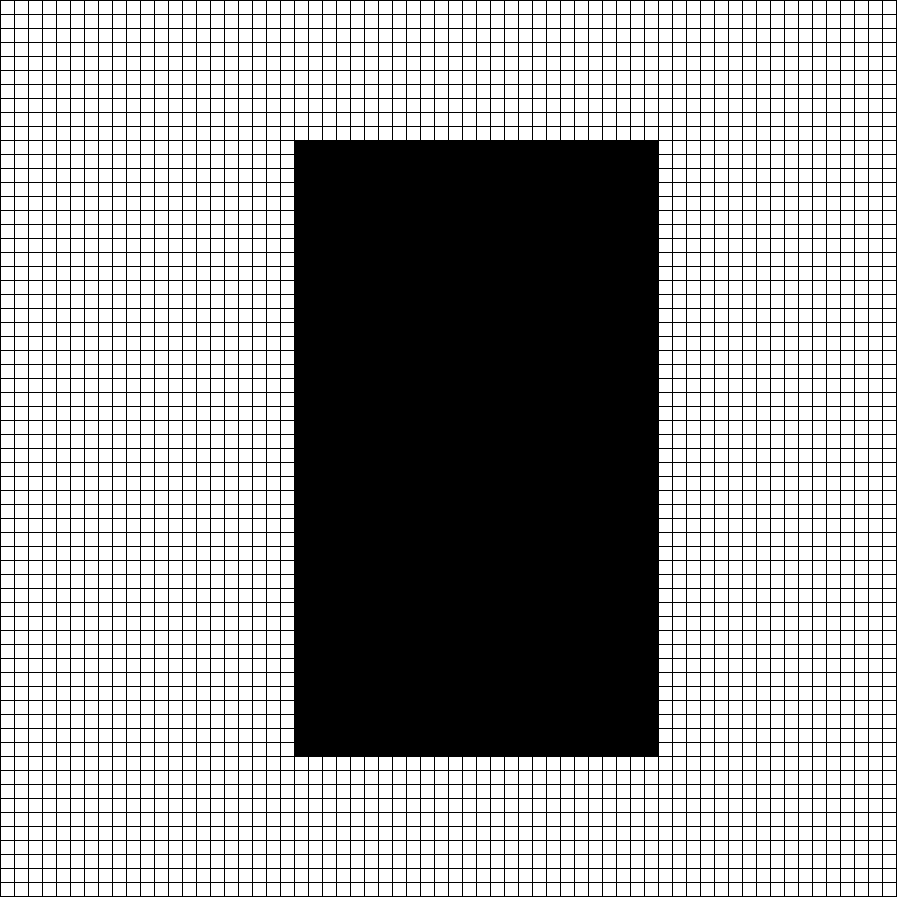
\includegraphics[scale=0.82]{images/m2.png}
    \caption{Block Map}
    \label{fig: rep_Block Map}
\end{figure}

\begin{table}[h!] 
\footnotesize
\centering


\begin{tabular}{|cc|c|c|c|c|c|}
\hline
\multicolumn{2}{|c|}{\textbf{Nr.}} & \textbf{Success Rate} & \textbf{Distance} & \textbf{Time} & \textbf{Distance Left}\\
\hline
\hline
\multicolumn{2}{|c|}{\cellcolor{lightgray!20} \hyperref[tab: evalalgorithms]{0}} & 100.0\% (I: 0\%) & 42.22 (A*: 42.22) (I: 0\%) & 0.0502s & 0.0\\
\hline
\hline
\multicolumn{2}{|c|}{\cellcolor{red!40} \hyperref[tab: evalalgorithms]{1}} & 52.0\% (I: -48.0\%) & 27.13 (A*: 27.07) (I: -0.22\%) & 0.0975s & 14.45\\
\hline
\multicolumn{2}{|c|}{\cellcolor{red!20} \hyperref[tab: evalalgorithms]{2}} & 98.0\% (I: -2.0\%) & 48.12 (A*: 41.82) (I: -15.06\%) & 0.1539s & 0.78\\
\hline
\multicolumn{2}{|c|}{\cellcolor{red!20} \hyperref[tab: evalalgorithms]{3}} & 94.0\% (I: -6.0\%) & 51.18 (A*: 41.05) (I: -24.68\%) & 0.1574s & 2.34\\
\hline
\multicolumn{2}{|c|}{\cellcolor{red!20} \hyperref[tab: evalalgorithms]{4}} & 100.0\% (I: 0\%) & 46.34 (A*: 42.22) (I: -9.76\%) & 0.1331s & 0.0\\
\hline
\multicolumn{2}{|c|}{\cellcolor{red!20} \hyperref[tab: evalalgorithms]{5}} & 100.0\% (I: 0\%) & 52.59 (A*: 42.22) (I: -24.56\%) & 0.1612s & 0.0\\
\hline
\hline
\multicolumn{2}{|c|}{\cellcolor{blue!20} \hyperref[tab: evalalgorithms]{6}} & 42.0\% (I: -58.0\%) & 22.62 (A*: 21.92) (I: -3.19\%) & 0.1171s & 17.19\\
\hline
\multicolumn{2}{|c|}{\cellcolor{blue!40} \hyperref[tab: evalalgorithms]{7}} & 96.0\% (I: -4.0\%) & 43.58 (A*: 41.64) (I: -4.66\%) & 0.1734s & 1.58\\
\hline
\multicolumn{2}{|c|}{\cellcolor{blue!20} \hyperref[tab: evalalgorithms]{8}} & 82.0\% (I: -18.0\%) & 42.86 (A*: 38.08) (I: -12.55\%) & 0.1667s & 6.99\\
\hline
\multicolumn{2}{|c|}{\cellcolor{blue!20} \hyperref[tab: evalalgorithms]{9}} & 100.0\% (I: 0\%) & 43.97 (A*: 42.22) (I: -4.14\%) & 0.1771s & 0.0\\
\hline
\multicolumn{2}{|c|}{\cellcolor{blue!20} \hyperref[tab: evalalgorithms]{10}} & 100.0\% (I: 0\%) & 53.48 (A*: 42.22) (I: -26.67\%) & 0.2055s & 0.0\\
\hline
\hline
\multicolumn{2}{|c|}{\cellcolor{orange!40} \hyperref[tab: evalalgorithms]{11}} & 100.0\% (I: 0\%) & 43.33 (A*: 42.22) (I: -2.63\%) & 1.8773s & 0.0\\
\hline
\hline
\multicolumn{1}{|M{0.15cm}}{\cellcolor{cyan!40}} & \multicolumn{1}{M{0.15cm}|}{\cellcolor{blue!40} \hspace*{-0.5cm}\hyperref[tab: evalalgorithms]{12}} & 100.0\% (I: 0\%) & 46.17 (A*: 42.22) (I: -9.36\%) & 0.5092s & 0.0\\
\hline
\multicolumn{1}{|M{0.15cm}}{\cellcolor{cyan!40}} & \multicolumn{1}{M{0.15cm}|}{\cellcolor{red!40} \hspace*{-0.5cm}\hyperref[tab: evalalgorithms]{13}} & 100.0\% (I: 0\%) & 106.16 (A*: 42.22) (I: -151.44\%) & 0.4863s & 0.0\\
\hline
\multicolumn{1}{|M{0.15cm}}{\cellcolor{cyan!40}} & \multicolumn{1}{M{0.15cm}|}{\cellcolor{orange!40} \hspace*{-0.5cm}\hyperref[tab: evalalgorithms]{14}} & 100.0\% (I: 0\%) & 49.25 (A*: 42.22) (I: -16.65\%) & 2.8345s & 0.0\\
\hline
\end{tabular}


\bigskip

\begin{tabular}{|cc|c|c|}
\hline
\multicolumn{2}{|c|}{\textbf{Nr.}} & \textbf{Pick Ratio}\\
\hline
\hline
\multicolumn{2}{|c|}{\cellcolor{orange!40} \hyperref[tab: evalalgorithms]{11}} & [86.0, 0.0, 0.0, 4.0, 2.0, 0.0, 0.0, 0.0, 6.0, 2.0]\%\\
\hline
\hline
\multicolumn{1}{|M{0.15cm}}{\cellcolor{cyan!40}} & \multicolumn{1}{M{0.15cm}|}{\cellcolor{orange!40} \hspace*{-0.5cm}\hyperref[tab: evalalgorithms]{14}} & [99.38, 0.62, 0.0, 0.0, 0.0, 0.0, 0.0, 0.0, 0.0, 0.0]\%\\
\hline
\end{tabular}


\bigskip

\begin{tabular}{|cc|c|c|c|c|M{3cm}|}
\hline
\multicolumn{2}{|c|}{\textbf{Nr.}} & \textbf{GK Improvement} & \textbf{GK Distance} & \textbf{GK Distance Left} & \textbf{WP} & \textbf{WP In-Between Distance}\\
\hline
\hline
\multicolumn{1}{|M{0.15cm}}{\cellcolor{cyan!40}} & \multicolumn{1}{M{0.15cm}|}{\cellcolor{blue!40} \hspace*{-0.5cm}\hyperref[tab: evalalgorithms]{12}} & 96.33\% & 44.11 & 1.58 & 3.7 & 15.73\\
\hline
\multicolumn{1}{|M{0.15cm}}{\cellcolor{cyan!40}} & \multicolumn{1}{M{0.15cm}|}{\cellcolor{red!40} \hspace*{-0.5cm}\hyperref[tab: evalalgorithms]{13}} & 91.14\% & 84.58 & 11.65 & 5.36 & 17.45\\
\hline
\multicolumn{1}{|M{0.15cm}}{\cellcolor{cyan!40}} & \multicolumn{1}{M{0.15cm}|}{\cellcolor{orange!40} \hspace*{-0.5cm}\hyperref[tab: evalalgorithms]{14}} & 100.0\% & 49.25 & 0.0 & 3.78 & 16.41\\
\hline
\end{tabular}


\bigskip

\begin{tabular}{|cc|c|c|c|c|c|}
\hline
\multicolumn{2}{|c|}{\textbf{Nr.}} & \textbf{Total Search} & \textbf{Total Fringe} & \textbf{Session Search} & \textbf{Session Fringe}\\
\hline
\hline
\multicolumn{2}{|c|}{\cellcolor{lightgray!20} \hyperref[tab: evalalgorithms]{0}} & 12.95\% & 3.02\% & 12.95\% & 3.02\%\\
\hline
\hline
\multicolumn{1}{|M{0.15cm}}{\cellcolor{cyan!40}} & \multicolumn{1}{M{0.15cm}|}{\cellcolor{blue!40} \hspace*{-0.5cm}\hyperref[tab: evalalgorithms]{12}} & 5.65\% (I: 56.37\%) & 2.62\% (I: 13.25\%) & 1.67\% (I: 87.1\%) & 0.85\% (I: 71.85\%)\\
\hline
\multicolumn{1}{|M{0.15cm}}{\cellcolor{cyan!40}} & \multicolumn{1}{M{0.15cm}|}{\cellcolor{red!40} \hspace*{-0.5cm}\hyperref[tab: evalalgorithms]{13}} & 11.35\% (I: 12.36\%) & 3.42\% (I: -13.25\%) & 2.29\% (I: 82.32\%) & 0.95\% (I: 68.54\%)\\
\hline
\multicolumn{1}{|M{0.15cm}}{\cellcolor{cyan!40}} & \multicolumn{1}{M{0.15cm}|}{\cellcolor{orange!40} \hspace*{-0.5cm}\hyperref[tab: evalalgorithms]{14}} & 5.48\% (I: 57.68\%) & 2.65\% (I: 12.25\%) & 1.63\% (I: 87.41\%) & 0.85\% (I: 71.85\%)\\
\hline
\end{tabular}


\caption{\textbf{Analyser} complex analysis on the block map described in Figure \ref{fig: rep_Block Map} with 50 random agent/goal positions}
\label{tab: eval_complex_analysis_map_2} 
\end{table}

\begin{itemize}
    \item Algorithm \hyperref[tab: evalalgorithms]{1} - better success rate due to the simplicity of the environment
    \item Algorithm \hyperref[tab: evalalgorithms]{7} - has high success rate because it has been trained on the same type of environment, and good distance improvement rate (the results are similar to paper \cite{inoue2019robot})
    \item Algorithm \hyperref[tab: evalalgorithms]{11} - has same success rate as A* and really good distance improvement rate
    \item Algorithm \hyperref[tab: evalalgorithms]{14} - GK Improvement is maximal, search space reduction is higher and the CAE Online LSTM Planner that was trained on the same type of maps is favoured
\end{itemize}

\pagebreak
\clearpage

\begin{figure}[h!]
    \centering
    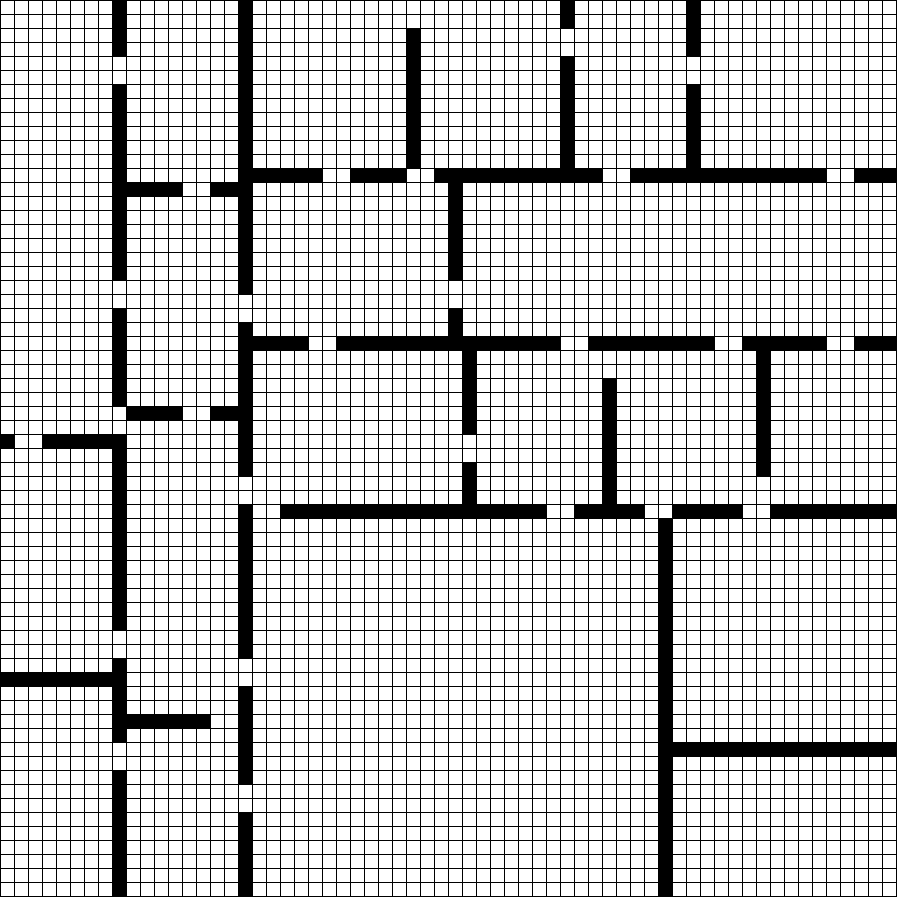
\includegraphics[scale=0.82]{images/m3.png}
    \caption{House Map}
    \label{fig: rep_House Map}
\end{figure}

\begin{table}[h!] 
\footnotesize
\centering


\begin{tabular}{|cc|c|c|c|c|c|}
\hline
\multicolumn{2}{|c|}{\textbf{Nr.}} & \textbf{Success Rate} & \textbf{Distance} & \textbf{Time} & \textbf{Distance Left}\\
\hline
\hline
\multicolumn{2}{|c|}{\cellcolor{lightgray!20} \hyperref[tab: evalalgorithms]{0}} & 96.0\% (I: 0\%) & 51.46 (A*: 51.46) (I: 0\%) & 0.0527s & 2.44\\
\hline
\hline
\multicolumn{2}{|c|}{\cellcolor{red!40} \hyperref[tab: evalalgorithms]{1}} & 6.0\% (I: -93.75\%) & 18.89 (A*: 18.61) (I: -1.5\%) & 0.0394s & 25.72\\
\hline
\multicolumn{2}{|c|}{\cellcolor{red!20} \hyperref[tab: evalalgorithms]{2}} & 6.0\% (I: -93.75\%) & 25.88 (A*: 24.38) (I: -6.15\%) & 0.0571s & 19.22\\
\hline
\multicolumn{2}{|c|}{\cellcolor{red!20} \hyperref[tab: evalalgorithms]{3}} & 72.0\% (I: -25.0\%) & 56.14 (A*: 47.45) (I: -18.31\%) & 0.1198s & 11.31\\
\hline
\multicolumn{2}{|c|}{\cellcolor{red!20} \hyperref[tab: evalalgorithms]{4}} & 4.0\% (I: -95.83\%) & 15.73 (A*: 15.73) (I: 0\%) & 0.0333s & 17.32\\
\hline
\multicolumn{2}{|c|}{\cellcolor{red!20} \hyperref[tab: evalalgorithms]{5}} & 40.0\% (I: -58.33\%) & 53.35 (A*: 45.25) (I: -17.9\%) & 0.1218s & 16.78\\
\hline
\hline
\multicolumn{2}{|c|}{\cellcolor{blue!20} \hyperref[tab: evalalgorithms]{6}} & 4.0\% (I: -95.83\%) & 15.73 (A*: 15.73) (I: 0\%) & 0.068s & 22.68\\
\hline
\multicolumn{2}{|c|}{\cellcolor{blue!40} \hyperref[tab: evalalgorithms]{7}} & 2.0\% (I: -97.92\%) & 8.07 (A*: 8.07) (I: 0\%) & 0.0536s & 29.76\\
\hline
\multicolumn{2}{|c|}{\cellcolor{blue!20} \hyperref[tab: evalalgorithms]{8}} & 46.0\% (I: -52.08\%) & 56.98 (A*: 46.91) (I: -21.47\%) & 0.152s & 19.01\\
\hline
\multicolumn{2}{|c|}{\cellcolor{blue!20} \hyperref[tab: evalalgorithms]{9}} & 4.0\% (I: -95.83\%) & 15.73 (A*: 15.73) (I: 0\%) & 0.0685s & 17.47\\
\hline
\multicolumn{2}{|c|}{\cellcolor{blue!20} \hyperref[tab: evalalgorithms]{10}} & 54.0\% (I: -43.75\%) & 65.4 (A*: 55.07) (I: -18.76\%) & 0.236s & 10.38\\
\hline
\hline
\multicolumn{2}{|c|}{\cellcolor{orange!40} \hyperref[tab: evalalgorithms]{11}} & 84.0\% (I: -12.5\%) & 58.41 (A*: 50.28) (I: -16.17\%) & 1.3005s & 4.14\\
\hline
\hline
\multicolumn{1}{|M{0.15cm}}{\cellcolor{cyan!40}} & \multicolumn{1}{M{0.15cm}|}{\cellcolor{blue!40} \hspace*{-0.5cm}\hyperref[tab: evalalgorithms]{12}} & 96.0\% (I: 0\%) & 57.91 (A*: 51.46) (I: -12.53\%) & 0.5204s & 2.16\\
\hline
\multicolumn{1}{|M{0.15cm}}{\cellcolor{cyan!40}} & \multicolumn{1}{M{0.15cm}|}{\cellcolor{red!40} \hspace*{-0.5cm}\hyperref[tab: evalalgorithms]{13}} & 96.0\% (I: 0\%) & 59.51 (A*: 51.46) (I: -15.64\%) & 0.2932s & 2.2\\
\hline
\multicolumn{1}{|M{0.15cm}}{\cellcolor{cyan!40}} & \multicolumn{1}{M{0.15cm}|}{\cellcolor{orange!40} \hspace*{-0.5cm}\hyperref[tab: evalalgorithms]{14}} & 96.0\% (I: 0\%) & 58.51 (A*: 51.46) (I: -13.7\%) & 2.8492s & 2.17\\
\hline
\end{tabular}


\bigskip

\begin{tabular}{|cc|c|c|}
\hline
\multicolumn{2}{|c|}{\textbf{Nr.}} & \textbf{Pick Ratio}\\
\hline
\hline
\multicolumn{2}{|c|}{\cellcolor{orange!40} \hyperref[tab: evalalgorithms]{11}} & [6.0, 2.0, 22.0, 24.0, 6.0, 0.0, 2.0, 38.0, 0.0, 0.0]\%\\
\hline
\hline
\multicolumn{1}{|M{0.15cm}}{\cellcolor{cyan!40}} & \multicolumn{1}{M{0.15cm}|}{\cellcolor{orange!40} \hspace*{-0.5cm}\hyperref[tab: evalalgorithms]{14}} & [35.44, 20.73, 22.16, 3.17, 3.33, 1.0, 0.67, 13.17, 0.33, 0.0]\%\\
\hline
\end{tabular}


\bigskip

\begin{tabular}{|cc|c|c|c|c|M{3cm}|}
\hline
\multicolumn{2}{|c|}{\textbf{Nr.}} & \textbf{GK Improvement} & \textbf{GK Distance} & \textbf{GK Distance Left} & \textbf{WP} & \textbf{WP In-Between Distance}\\
\hline
\hline
\multicolumn{1}{|M{0.15cm}}{\cellcolor{cyan!40}} & \multicolumn{1}{M{0.15cm}|}{\cellcolor{blue!40} \hspace*{-0.5cm}\hyperref[tab: evalalgorithms]{12}} & 48.3\% & 26.29 & 25.91 & 7.54 & 3.65\\
\hline
\multicolumn{1}{|M{0.15cm}}{\cellcolor{cyan!40}} & \multicolumn{1}{M{0.15cm}|}{\cellcolor{red!40} \hspace*{-0.5cm}\hyperref[tab: evalalgorithms]{13}} & 71.9\% & 41.14 & 14.11 & 5.44 & 9.26\\
\hline
\multicolumn{1}{|M{0.15cm}}{\cellcolor{cyan!40}} & \multicolumn{1}{M{0.15cm}|}{\cellcolor{orange!40} \hspace*{-0.5cm}\hyperref[tab: evalalgorithms]{14}} & 96.77\% & 58.79 & 3.61 & 4.22 & 16.36\\
\hline
\end{tabular}


\bigskip

\begin{tabular}{|cc|c|c|c|c|c|}
\hline
\multicolumn{2}{|c|}{\textbf{Nr.}} & \textbf{Total Search} & \textbf{Total Fringe} & \textbf{Session Search} & \textbf{Session Fringe}\\
\hline
\hline
\multicolumn{2}{|c|}{\cellcolor{lightgray!20} \hyperref[tab: evalalgorithms]{0}} & 16.69\% & 4.94\% & 16.69\% & 4.94\%\\
\hline
\hline
\multicolumn{1}{|M{0.15cm}}{\cellcolor{cyan!40}} & \multicolumn{1}{M{0.15cm}|}{\cellcolor{blue!40} \hspace*{-0.5cm}\hyperref[tab: evalalgorithms]{12}} & 10.42\% (I: 37.57\%) & 4.21\% (I: 14.78\%) & 1.56\% (I: 90.65\%) & 0.7\% (I: 85.83\%)\\
\hline
\multicolumn{1}{|M{0.15cm}}{\cellcolor{cyan!40}} & \multicolumn{1}{M{0.15cm}|}{\cellcolor{red!40} \hspace*{-0.5cm}\hyperref[tab: evalalgorithms]{13}} & 10.15\% (I: 39.19\%) & 4.12\% (I: 16.6\%) & 2.07\% (I: 87.6\%) & 0.95\% (I: 80.77\%)\\
\hline
\multicolumn{1}{|M{0.15cm}}{\cellcolor{cyan!40}} & \multicolumn{1}{M{0.15cm}|}{\cellcolor{orange!40} \hspace*{-0.5cm}\hyperref[tab: evalalgorithms]{14}} & 9.8\% (I: 41.28\%) & 4.49\% (I: 9.11\%) & 2.58\% (I: 84.54\%) & 1.3\% (I: 73.68\%)\\
\hline
\end{tabular}


\caption{\textbf{Analyser} complex analysis on the house map described in Figure \ref{fig: rep_House Map} with 50 random agent/goal positions}
\label{tab: eval_complex_analysis_map_3} 
\end{table}

\begin{itemize}
    \item Algorithm \hyperref[tab: evalalgorithms]{1} - performance is severely impacted
    \item Algorithm \hyperref[tab: evalalgorithms]{7} - performance is severely impacted
    \item Algorithm \hyperref[tab: evalalgorithms]{11} - good Success Rate, but worse distance improvement rate
    \item Algorithm \hyperref[tab: evalalgorithms]{14} - great GK Improvement, same distance improvement rate and good search space reduction
\end{itemize}

\pagebreak
\clearpage

\begin{figure}[h!]
    \centering
    
\includegraphics[scale=0.82]{images/m4.png}
    \caption{Hand Crafted Map 1}
    \label{fig: rep_Hand Crafted Map 1}
\end{figure}


\begin{table}[h!] 
\footnotesize
\centering


\begin{tabular}{|cc|c|c|c|c|c|}
\hline
\multicolumn{2}{|c|}{\textbf{Nr.}} & \textbf{Success Rate} & \textbf{Distance} & \textbf{Time} & \textbf{Distance Left}\\
\hline
\hline
\multicolumn{2}{|c|}{\cellcolor{lightgray!20} \hyperref[tab: evalalgorithms]{0}} & 100.0\% (I: 0\%) & 18.95 (A*: 18.95) (I: 0\%) & 0.0212s & 0.0\\
\hline
\hline
\multicolumn{2}{|c|}{\cellcolor{red!40} \hyperref[tab: evalalgorithms]{1}} & 22.0\% (I: -78.0\%) & 6.65 (A*: 6.65) (I: 0\%) & 0.0256s & 2.56\\
\hline
\multicolumn{2}{|c|}{\cellcolor{red!20} \hyperref[tab: evalalgorithms]{2}} & 42.0\% (I: -58.0\%) & 12.41 (A*: 11.54) (I: -7.54\%) & 0.0409s & 2.72\\
\hline
\multicolumn{2}{|c|}{\cellcolor{red!20} \hyperref[tab: evalalgorithms]{3}} & 38.0\% (I: -62.0\%) & 15.13 (A*: 15.03) (I: -0.67\%) & 0.0526s & 2.69\\
\hline
\multicolumn{2}{|c|}{\cellcolor{red!20} \hyperref[tab: evalalgorithms]{4}} & 46.0\% (I: -54.0\%) & 12.67 (A*: 12.13) (I: -4.45\%) & 0.0404s & 1.08\\
\hline
\multicolumn{2}{|c|}{\cellcolor{red!20} \hyperref[tab: evalalgorithms]{5}} & 60.0\% (I: -40.0\%) & 16.97 (A*: 15.1) (I: -12.38\%) & 0.0458s & 1.46\\
\hline
\hline
\multicolumn{2}{|c|}{\cellcolor{blue!20} \hyperref[tab: evalalgorithms]{6}} & 24.0\% (I: -76.0\%) & 6.91 (A*: 6.91) (I: 0\%) & 0.0438s & 3.24\\
\hline
\multicolumn{2}{|c|}{\cellcolor{blue!40} \hyperref[tab: evalalgorithms]{7}} & 44.0\% (I: -56.0\%) & 12.12 (A*: 11.45) (I: -5.85\%) & 0.0693s & 1.65\\
\hline
\multicolumn{2}{|c|}{\cellcolor{blue!20} \hyperref[tab: evalalgorithms]{8}} & 42.0\% (I: -58.0\%) & 14.53 (A*: 13.44) (I: -8.11\%) & 0.0673s & 4.39\\
\hline
\multicolumn{2}{|c|}{\cellcolor{blue!20} \hyperref[tab: evalalgorithms]{9}} & 14.0\% (I: -86.0\%) & 5.71 (A*: 5.51) (I: -3.63\%) & 0.0476s & 3.44\\
\hline
\multicolumn{2}{|c|}{\cellcolor{blue!20} \hyperref[tab: evalalgorithms]{10}} & 36.0\% (I: -64.0\%) & 11.24 (A*: 9.75) (I: -15.28\%) & 0.0704s & 1.7\\
\hline
\hline
\multicolumn{2}{|c|}{\cellcolor{orange!40} \hyperref[tab: evalalgorithms]{11}} & 72.0\% (I: -28.0\%) & 18.62 (A*: 16.52) (I: -12.71\%) & 0.727s & 0.99\\
\hline
\hline
\multicolumn{1}{|M{0.15cm}}{\cellcolor{cyan!40}} & \multicolumn{1}{M{0.15cm}|}{\cellcolor{blue!40} \hspace*{-0.5cm}\hyperref[tab: evalalgorithms]{12}} & 100.0\% (I: 0\%) & 23.74 (A*: 18.95) (I: -25.28\%) & 0.2857s & 0.0\\
\hline
\multicolumn{1}{|M{0.15cm}}{\cellcolor{cyan!40}} & \multicolumn{1}{M{0.15cm}|}{\cellcolor{red!40} \hspace*{-0.5cm}\hyperref[tab: evalalgorithms]{13}} & 100.0\% (I: 0\%) & 42.72 (A*: 18.95) (I: -125.44\%) & 0.2533s & 0.0\\
\hline
\multicolumn{1}{|M{0.15cm}}{\cellcolor{cyan!40}} & \multicolumn{1}{M{0.15cm}|}{\cellcolor{orange!40} \hspace*{-0.5cm}\hyperref[tab: evalalgorithms]{14}} & 100.0\% (I: 0\%) & 46.86 (A*: 18.95) (I: -147.28\%) & 2.6125s & 0.0\\
\hline
\end{tabular}


\bigskip

\begin{tabular}{|cc|c|c|}
\hline
\multicolumn{2}{|c|}{\textbf{Nr.}} & \textbf{Pick Ratio}\\
\hline
\hline
\multicolumn{2}{|c|}{\cellcolor{orange!40} \hyperref[tab: evalalgorithms]{11}} & [26.0, 2.0, 18.0, 4.0, 0.0, 0.0, 4.0, 20.0, 18.0, 8.0]\%\\
\hline
\hline
\multicolumn{1}{|M{0.15cm}}{\cellcolor{cyan!40}} & \multicolumn{1}{M{0.15cm}|}{\cellcolor{orange!40} \hspace*{-0.5cm}\hyperref[tab: evalalgorithms]{14}} & [34.87, 2.0, 29.33, 5.76, 0.0, 0.0, 2.0, 13.68, 11.36, 1.0]\%\\
\hline
\end{tabular}


\bigskip

\begin{tabular}{|cc|c|c|c|c|M{3cm}|}
\hline
\multicolumn{2}{|c|}{\textbf{Nr.}} & \textbf{GK Improvement} & \textbf{GK Distance} & \textbf{GK Distance Left} & \textbf{WP} & \textbf{WP In-Between Distance}\\
\hline
\hline
\multicolumn{1}{|M{0.15cm}}{\cellcolor{cyan!40}} & \multicolumn{1}{M{0.15cm}|}{\cellcolor{blue!40} \hspace*{-0.5cm}\hyperref[tab: evalalgorithms]{12}} & 53.21\% & 8.42 & 1.65 & 4.24 & 4.7\\
\hline
\multicolumn{1}{|M{0.15cm}}{\cellcolor{cyan!40}} & \multicolumn{1}{M{0.15cm}|}{\cellcolor{red!40} \hspace*{-0.5cm}\hyperref[tab: evalalgorithms]{13}} & 88.32\% & 31.88 & 0.73 & 4.98 & 7.98\\
\hline
\multicolumn{1}{|M{0.15cm}}{\cellcolor{cyan!40}} & \multicolumn{1}{M{0.15cm}|}{\cellcolor{orange!40} \hspace*{-0.5cm}\hyperref[tab: evalalgorithms]{14}} & 95.02\% & 41.05 & 0.65 & 5.2 & 8.93\\
\hline
\end{tabular}


\bigskip

\begin{tabular}{|cc|c|c|c|c|c|}
\hline
\multicolumn{2}{|c|}{\textbf{Nr.}} & \textbf{Total Search} & \textbf{Total Fringe} & \textbf{Session Search} & \textbf{Session Fringe}\\
\hline
\hline
\multicolumn{2}{|c|}{\cellcolor{lightgray!20} \hyperref[tab: evalalgorithms]{0}} & 36.47\% & 7.18\% & 36.47\% & 7.18\%\\
\hline
\hline
\multicolumn{1}{|M{0.15cm}}{\cellcolor{cyan!40}} & \multicolumn{1}{M{0.15cm}|}{\cellcolor{blue!40} \hspace*{-0.5cm}\hyperref[tab: evalalgorithms]{12}} & 40.77\% (I: -11.79\%) & 8.82\% (I: -22.84\%) & 9.33\% (I: 74.42\%) & 2.65\% (I: 63.09\%)\\
\hline
\multicolumn{1}{|M{0.15cm}}{\cellcolor{cyan!40}} & \multicolumn{1}{M{0.15cm}|}{\cellcolor{red!40} \hspace*{-0.5cm}\hyperref[tab: evalalgorithms]{13}} & 43.34\% (I: -18.84\%) & 10.45\% (I: -45.54\%) & 10.09\% (I: 72.33\%) & 3.47\% (I: 51.67\%)\\
\hline
\multicolumn{1}{|M{0.15cm}}{\cellcolor{cyan!40}} & \multicolumn{1}{M{0.15cm}|}{\cellcolor{orange!40} \hspace*{-0.5cm}\hyperref[tab: evalalgorithms]{14}} & 46.3\% (I: -26.95\%) & 14.3\% (I: -99.16\%) & 11.62\% (I: 68.14\%) & 4.33\% (I: 39.69\%)\\
\hline
\end{tabular}


\caption{\textbf{Analyser} complex analysis on the hand crafted map described in Figure \ref{fig: rep_Hand Crafted Map 1} with 50 random agent/goal positions}
\label{tab: eval_complex_analysis_map_4} 
\end{table}

\begin{itemize}
    \item Algorithm \hyperref[tab: evalalgorithms]{1} - performance is worse
    \item Algorithm \hyperref[tab: evalalgorithms]{7} - performance is similar
    \item Algorithm \hyperref[tab: evalalgorithms]{11} - Success Rate is a bit lower and distance improvement is worse as well
    \item Algorithm \hyperref[tab: evalalgorithms]{14} - great GK Improvement, but severely impacted distance improvement rate (-147.28\%). This is a sign that the global kernel goes around the whole obstacle until it finds the entrance. Other metrics are badly affected as well. Since Algorithm \hyperref[tab: evalalgorithms]{11} has relatively similar performance, increasing the $gk\_max\_it$ might improve the distance improvement rate
\end{itemize}

\pagebreak
\clearpage

\begin{figure}[h!]
    \centering
    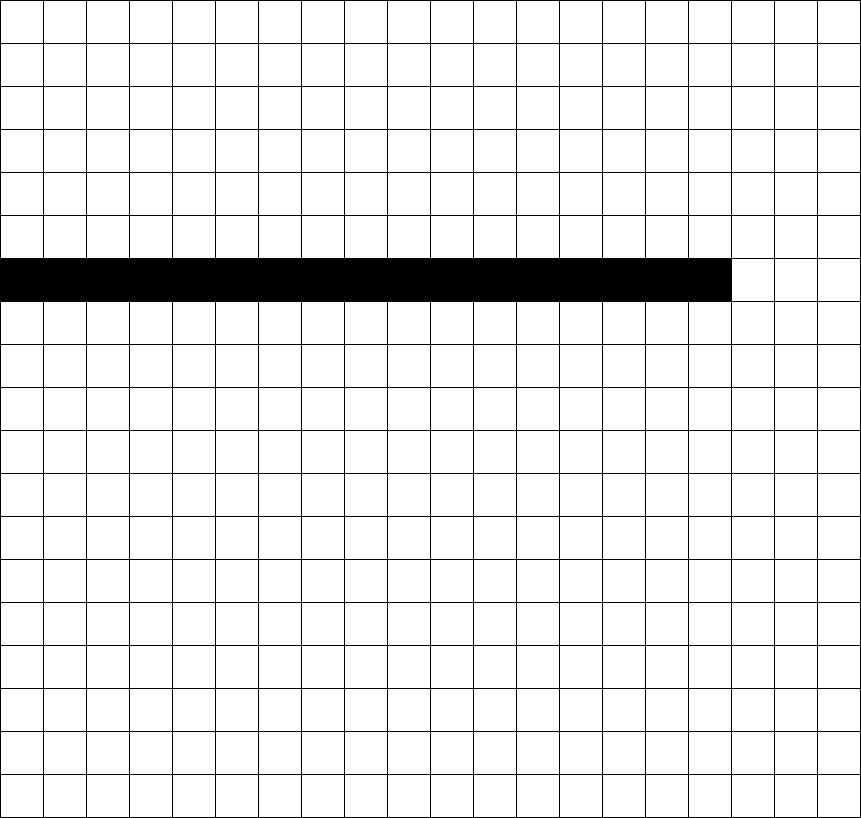
\includegraphics[scale=0.82]{images/m5.png}
    \caption{Hand Crafted Map 2}
    \label{fig: rep_Hand Crafted Map 2}
\end{figure}

\begin{table}[h!] 
\footnotesize
\centering


\begin{tabular}{|cc|c|c|c|c|c|}
\hline
\multicolumn{2}{|c|}{\textbf{Nr.}} & \textbf{Success Rate} & \textbf{Distance} & \textbf{Time} & \textbf{Distance Left}\\
\hline
\hline
\multicolumn{2}{|c|}{\cellcolor{lightgray!20} \hyperref[tab: evalalgorithms]{0}} & 100.0\% (I: 0\%) & 10.24 (A*: 10.24) (I: 0\%) & 0.0055s & 0.0\\
\hline
\hline
\multicolumn{2}{|c|}{\cellcolor{red!40} \hyperref[tab: evalalgorithms]{1}} & 78.0\% (I: -22.0\%) & 7.5 (A*: 7.48) (I: -0.27\%) & 0.02s & 2.04\\
\hline
\multicolumn{2}{|c|}{\cellcolor{red!20} \hyperref[tab: evalalgorithms]{2}} & 80.0\% (I: -20.0\%) & 8.05 (A*: 7.92) (I: -1.64\%) & 0.0206s & 2.01\\
\hline
\multicolumn{2}{|c|}{\cellcolor{red!20} \hyperref[tab: evalalgorithms]{3}} & 98.0\% (I: -2.0\%) & 10.15 (A*: 10.09) (I: -0.59\%) & 0.0255s & 0.16\\
\hline
\multicolumn{2}{|c|}{\cellcolor{red!20} \hyperref[tab: evalalgorithms]{4}} & 78.0\% (I: -22.0\%) & 7.48 (A*: 7.48) (I: 0\%) & 0.0196s & 1.77\\
\hline
\multicolumn{2}{|c|}{\cellcolor{red!20} \hyperref[tab: evalalgorithms]{5}} & 98.0\% (I: -2.0\%) & 10.22 (A*: 10.17) (I: -0.49\%) & 0.0253s & 0.32\\
\hline
\hline
\multicolumn{2}{|c|}{\cellcolor{blue!20} \hyperref[tab: evalalgorithms]{6}} & 78.0\% (I: -22.0\%) & 7.89 (A*: 7.48) (I: -5.48\%) & 0.0429s & 1.77\\
\hline
\multicolumn{2}{|c|}{\cellcolor{blue!40} \hyperref[tab: evalalgorithms]{7}} & 76.0\% (I: -24.0\%) & 7.89 (A*: 7.36) (I: -7.2\%) & 0.0434s & 1.97\\
\hline
\multicolumn{2}{|c|}{\cellcolor{blue!20} \hyperref[tab: evalalgorithms]{8}} & 96.0\% (I: -4.0\%) & 10.16 (A*: 10.13) (I: -0.3\%) & 0.0481s & 0.34\\
\hline
\multicolumn{2}{|c|}{\cellcolor{blue!20} \hyperref[tab: evalalgorithms]{9}} & 76.0\% (I: -24.0\%) & 7.36 (A*: 7.36) (I: 0\%) & 0.0423s & 1.92\\
\hline
\multicolumn{2}{|c|}{\cellcolor{blue!20} \hyperref[tab: evalalgorithms]{10}} & 100.0\% (I: 0\%) & 10.31 (A*: 10.24) (I: -0.68\%) & 0.0485s & 0.0\\
\hline
\hline
\multicolumn{2}{|c|}{\cellcolor{orange!40} \hyperref[tab: evalalgorithms]{11}} & 100.0\% (I: 0\%) & 10.35 (A*: 10.24) (I: -1.07\%) & 0.4895s & 0.0\\
\hline
\multicolumn{1}{|M{0.15cm}}{\cellcolor{cyan!40}} & \multicolumn{1}{M{0.15cm}|}{\cellcolor{blue!40} \hspace*{-0.5cm}\hyperref[tab: evalalgorithms]{12}} & 100.0\% (I: 0\%) & 10.43 (A*: 10.24) (I: -1.86\%) & 0.1472s & 0.0\\
\hline
\multicolumn{1}{|M{0.15cm}}{\cellcolor{cyan!40}} & \multicolumn{1}{M{0.15cm}|}{\cellcolor{red!40} \hspace*{-0.5cm}\hyperref[tab: evalalgorithms]{13}} & 100.0\% (I: 0\%) & 10.87 (A*: 10.24) (I: -6.15\%) & 0.0548s & 0.0\\
\hline
\multicolumn{1}{|M{0.15cm}}{\cellcolor{cyan!40}} & \multicolumn{1}{M{0.15cm}|}{\cellcolor{orange!40} \hspace*{-0.5cm}\hyperref[tab: evalalgorithms]{14}} & 100.0\% (I: 0\%) & 10.24 (A*: 10.24) (I: 0\%) & 0.5487s & 0.0\\
\hline
\end{tabular}


\bigskip

\begin{tabular}{|cc|c|c|}
\hline
\multicolumn{2}{|c|}{\textbf{Nr.}} & \textbf{Pick Ratio}\\
\hline
\hline
\multicolumn{2}{|c|}{\cellcolor{orange!40} \hyperref[tab: evalalgorithms]{11}} & [72.0, 6.0, 20.0, 2.0, 0.0, 0.0, 0.0, 0.0, 0.0, 0.0]\%\\
\hline
\hline
\multicolumn{1}{|M{0.15cm}}{\cellcolor{cyan!40}} & \multicolumn{1}{M{0.15cm}|}{\cellcolor{orange!40} \hspace*{-0.5cm}\hyperref[tab: evalalgorithms]{14}} & [74.0, 8.0, 16.0, 2.0, 0.0, 0.0, 0.0, 0.0, 0.0, 0.0]\%\\
\hline
\end{tabular}


\bigskip

\begin{tabular}{|cc|c|c|c|c|M{3cm}|}
\hline
\multicolumn{2}{|c|}{\textbf{Nr.}} & \textbf{GK Improvement} & \textbf{GK Distance} & \textbf{GK Distance Left} & \textbf{WP} & \textbf{WP In-Between Distance}\\
\hline
\hline
\multicolumn{1}{|M{0.15cm}}{\cellcolor{cyan!40}} & \multicolumn{1}{M{0.15cm}|}{\cellcolor{blue!40} \hspace*{-0.5cm}\hyperref[tab: evalalgorithms]{12}} & 87.29\% & 8.0 & 1.97 & 3.02 & 5.64\\
\hline
\multicolumn{1}{|M{0.15cm}}{\cellcolor{cyan!40}} & \multicolumn{1}{M{0.15cm}|}{\cellcolor{red!40} \hspace*{-0.5cm}\hyperref[tab: evalalgorithms]{13}} & 100.0\% & 10.87 & 0.0 & 2.1 & 8.03\\
\hline
\multicolumn{1}{|M{0.15cm}}{\cellcolor{cyan!40}} & \multicolumn{1}{M{0.15cm}|}{\cellcolor{orange!40} \hspace*{-0.5cm}\hyperref[tab: evalalgorithms]{14}} & 100.0\% & 10.24 & 0.0 & 2.06 & 8.12\\
\hline
\end{tabular}


\bigskip

\begin{tabular}{|cc|c|c|c|c|c|}
\hline
\multicolumn{2}{|c|}{\textbf{Nr.}} & \textbf{Total Search} & \textbf{Total Fringe} & \textbf{Session Search} & \textbf{Session Fringe}\\
\hline
\hline
\multicolumn{2}{|c|}{\cellcolor{lightgray!20} \hyperref[tab: evalalgorithms]{0}} & 16.25\% & 8.17\% & 16.25\% & 8.17\%\\
\hline
\hline
\multicolumn{1}{|M{0.15cm}}{\cellcolor{cyan!40}} & \multicolumn{1}{M{0.15cm}|}{\cellcolor{blue!40} \hspace*{-0.5cm}\hyperref[tab: evalalgorithms]{12}} & 13.32\% (I: 18.03\%) & 7.85\% (I: 3.92\%) & 5.13\% (I: 68.43\%) & 3.22\% (I: 60.59\%)\\
\hline
\multicolumn{1}{|M{0.15cm}}{\cellcolor{cyan!40}} & \multicolumn{1}{M{0.15cm}|}{\cellcolor{red!40} \hspace*{-0.5cm}\hyperref[tab: evalalgorithms]{13}} & 15.88\% (I: 2.28\%) & 7.59\% (I: 7.1\%) & 7.93\% (I: 51.2\%) & 4.13\% (I: 49.45\%)\\
\hline
\multicolumn{1}{|M{0.15cm}}{\cellcolor{cyan!40}} & \multicolumn{1}{M{0.15cm}|}{\cellcolor{orange!40} \hspace*{-0.5cm}\hyperref[tab: evalalgorithms]{14}} & 14.94\% (I: 8.06\%) & 7.49\% (I: 8.32\%) & 7.71\% (I: 52.55\%) & 4.16\% (I: 49.08\%)\\
\hline
\end{tabular}


\caption{\textbf{Analyser} complex analysis on the hand crafted map described in Figure \ref{fig: rep_Hand Crafted Map 2} with 50 random agent/goal positions}
\label{tab: eval_complex_analysis_map_5} 
\end{table}

\begin{itemize}
    \item The performance of all algorithms is greatly boosted as the hand crafted map is quite simple in layout, but was used to test the ability of the algorithm to go around long walls which was an issue in paper \cite{nicola2018lstm}
    \item Algorithm \hyperref[tab: evalalgorithms]{14} - has 100\% GK Improvement and 0\% distance improvement rate, which matches the A* performance exactly
\end{itemize}

\pagebreak
\clearpage

\begin{figure}[h!]
    \centering
    
\includegraphics[scale=0.82]{images/m6.png}
    \caption{Hand Crafted Map 3}
    \label{fig: rep_Hand Crafted Map 3}
\end{figure}

\begin{table}[h!] 
\footnotesize
\centering


\begin{tabular}{|cc|c|c|c|c|c|}
\hline
\multicolumn{2}{|c|}{\textbf{Nr.}} & \textbf{Success Rate} & \textbf{Distance} & \textbf{Time} & \textbf{Distance Left}\\
\hline
\hline
\multicolumn{2}{|c|}{\cellcolor{lightgray!20} \hyperref[tab: evalalgorithms]{0}} & 100.0\% (I: 0\%) & 22.66 (A*: 22.66) (I: 0\%) & 0.0182s & 0.0\\
\hline
\hline
\multicolumn{2}{|c|}{\cellcolor{red!40} \hyperref[tab: evalalgorithms]{1}} & 76.0\% (I: -24.0\%) & 20.19 (A*: 20.09) (I: -0.5\%) & 0.0587s & 4.88\\
\hline
\multicolumn{2}{|c|}{\cellcolor{red!20} \hyperref[tab: evalalgorithms]{2}} & 98.0\% (I: -2.0\%) & 26.81 (A*: 22.59) (I: -18.68\%) & 0.0718s & 0.42\\
\hline
\multicolumn{2}{|c|}{\cellcolor{red!20} \hyperref[tab: evalalgorithms]{3}} & 74.0\% (I: -26.0\%) & 23.72 (A*: 20.14) (I: -17.78\%) & 0.0697s & 5.37\\
\hline
\multicolumn{2}{|c|}{\cellcolor{red!20} \hyperref[tab: evalalgorithms]{4}} & 84.0\% (I: -16.0\%) & 21.48 (A*: 21.21) (I: -1.27\%) & 0.0618s & 3.35\\
\hline
\multicolumn{2}{|c|}{\cellcolor{red!20} \hyperref[tab: evalalgorithms]{5}} & 96.0\% (I: -4.0\%) & 23.64 (A*: 22.34) (I: -5.82\%) & 0.0562s & 0.84\\
\hline
\hline
\multicolumn{2}{|c|}{\cellcolor{blue!20} \hyperref[tab: evalalgorithms]{6}} & 86.0\% (I: -14.0\%) & 21.52 (A*: 21.25) (I: -1.27\%) & 0.0835s & 2.94\\
\hline
\multicolumn{2}{|c|}{\cellcolor{blue!40} \hyperref[tab: evalalgorithms]{7}} & 76.0\% (I: -24.0\%) & 23.38 (A*: 20.25) (I: -15.46\%) & 0.0807s & 4.83\\
\hline
\multicolumn{2}{|c|}{\cellcolor{blue!20} \hyperref[tab: evalalgorithms]{8}} & 72.0\% (I: -28.0\%) & 20.67 (A*: 19.71) (I: -4.87\%) & 0.0729s & 6.11\\
\hline
\multicolumn{2}{|c|}{\cellcolor{blue!20} \hyperref[tab: evalalgorithms]{9}} & 90.0\% (I: -10.0\%) & 22.5 (A*: 22.01) (I: -2.23\%) & 0.0762s & 2.1\\
\hline
\multicolumn{2}{|c|}{\cellcolor{blue!20} \hyperref[tab: evalalgorithms]{10}} & 78.0\% (I: -22.0\%) & 20.97 (A*: 20.49) (I: -2.34\%) & 0.0728s & 4.23\\
\hline
\hline
\multicolumn{2}{|c|}{\cellcolor{orange!40} \hyperref[tab: evalalgorithms]{11}} & 100.0\% (I: 0\%) & 23.27 (A*: 22.66) (I: -2.69\%) & 0.6844s & 0.0\\
\hline
\hline
\multicolumn{1}{|M{0.15cm}}{\cellcolor{cyan!40}} & \multicolumn{1}{M{0.15cm}|}{\cellcolor{blue!40} \hspace*{-0.5cm}\hyperref[tab: evalalgorithms]{12}} & 100.0\% (I: 0\%) & 23.96 (A*: 22.66) (I: -5.74\%) & 0.164s & 0.0\\
\hline
\multicolumn{1}{|M{0.15cm}}{\cellcolor{cyan!40}} & \multicolumn{1}{M{0.15cm}|}{\cellcolor{red!40} \hspace*{-0.5cm}\hyperref[tab: evalalgorithms]{13}} & 100.0\% (I: 0\%) & 23.2 (A*: 22.66) (I: -2.38\%) & 0.1004s & 0.0\\
\hline
\multicolumn{1}{|M{0.15cm}}{\cellcolor{cyan!40}} & \multicolumn{1}{M{0.15cm}|}{\cellcolor{orange!40} \hspace*{-0.5cm}\hyperref[tab: evalalgorithms]{14}} & 100.0\% (I: 0\%) & 22.66 (A*: 22.66) (I: 0\%) & 1.0798s & 0.0\\
\hline
\end{tabular}


\bigskip

\begin{tabular}{|cc|c|c|}
\hline
\multicolumn{2}{|c|}{\textbf{Nr.}} & \textbf{Pick Ratio}\\
\hline
\hline
\multicolumn{2}{|c|}{\cellcolor{orange!40} \hyperref[tab: evalalgorithms]{11}} & [50.0, 38.0, 2.0, 0.0, 0.0, 2.0, 0.0, 4.0, 0.0, 4.0]\%\\
\hline
\hline
\multicolumn{1}{|M{0.15cm}}{\cellcolor{cyan!40}} & \multicolumn{1}{M{0.15cm}|}{\cellcolor{orange!40} \hspace*{-0.5cm}\hyperref[tab: evalalgorithms]{14}} & [63.0, 31.0, 2.0, 2.0, 0.0, 1.0, 1.0, 0.0, 0.0, 0.0]\%\\
\hline
\end{tabular}


\bigskip

\begin{tabular}{|cc|c|c|c|c|M{3cm}|}
\hline
\multicolumn{2}{|c|}{\textbf{Nr.}} & \textbf{GK Improvement} & \textbf{GK Distance} & \textbf{GK Distance Left} & \textbf{WP} & \textbf{WP In-Between Distance}\\
\hline
\hline
\multicolumn{1}{|M{0.15cm}}{\cellcolor{cyan!40}} & \multicolumn{1}{M{0.15cm}|}{\cellcolor{blue!40} \hspace*{-0.5cm}\hyperref[tab: evalalgorithms]{12}} & 81.99\% & 18.36 & 4.83 & 3.3 & 11.22\\
\hline
\multicolumn{1}{|M{0.15cm}}{\cellcolor{cyan!40}} & \multicolumn{1}{M{0.15cm}|}{\cellcolor{red!40} \hspace*{-0.5cm}\hyperref[tab: evalalgorithms]{13}} & 96.83\% & 22.14 & 0.84 & 2.6 & 14.37\\
\hline
\multicolumn{1}{|M{0.15cm}}{\cellcolor{cyan!40}} & \multicolumn{1}{M{0.15cm}|}{\cellcolor{orange!40} \hspace*{-0.5cm}\hyperref[tab: evalalgorithms]{14}} & 100.0\% & 22.66 & 0.0 & 2.44 & 14.98\\
\hline
\end{tabular}


\bigskip

\begin{tabular}{|cc|c|c|c|c|c|}
\hline
\multicolumn{2}{|c|}{\textbf{Nr.}} & \textbf{Total Search} & \textbf{Total Fringe} & \textbf{Session Search} & \textbf{Session Fringe}\\
\hline
\hline
\multicolumn{2}{|c|}{\cellcolor{lightgray!20} \hyperref[tab: evalalgorithms]{0}} & 19.46\% & 9.21\% & 19.46\% & 9.21\%\\
\hline
\hline
\multicolumn{1}{|M{0.15cm}}{\cellcolor{cyan!40}} & \multicolumn{1}{M{0.15cm}|}{\cellcolor{blue!40} \hspace*{-0.5cm}\hyperref[tab: evalalgorithms]{12}} & 14.93\% (I: 23.28\%) & 7.75\% (I: 15.85\%) & 5.43\% (I: 72.1\%) & 3.12\% (I: 66.12\%)\\
\hline
\multicolumn{1}{|M{0.15cm}}{\cellcolor{cyan!40}} & \multicolumn{1}{M{0.15cm}|}{\cellcolor{red!40} \hspace*{-0.5cm}\hyperref[tab: evalalgorithms]{13}} & 15.24\% (I: 21.69\%) & 7.87\% (I: 14.55\%) & 6.41\% (I: 67.06\%) & 3.63\% (I: 60.59\%)\\
\hline
\multicolumn{1}{|M{0.15cm}}{\cellcolor{cyan!40}} & \multicolumn{1}{M{0.15cm}|}{\cellcolor{orange!40} \hspace*{-0.5cm}\hyperref[tab: evalalgorithms]{14}} & 14.57\% (I: 25.13\%) & 7.53\% (I: 18.24\%) & 6.35\% (I: 67.37\%) & 3.59\% (I: 61.02\%)\\
\hline
\end{tabular}


\caption{\textbf{Analyser} complex analysis on the hand crafted map described in Figure \ref{fig: rep_Hand Crafted Map 3} with 50 random agent/goal positions}
\label{tab: eval_complex_analysis_map_6} 
\end{table}

\begin{itemize}
    \item The analysis has similar characteristics to the fifth complex analysis (See Table \ref{tab: eval_complex_analysis_map_5})
    \item Algorithm \hyperref[tab: evalalgorithms]{14} - has 100\% GK Improvement and 0\% distance improvement rate, which matches the A* performance exactly
\end{itemize}

\pagebreak
\clearpage

\begin{table}[h!] 
\small 
\centering


\begin{tabular}{|cc|c|c|c|c|c|}
\hline
\multicolumn{2}{|c|}{\textbf{Nr.}} & \textbf{Success Rate} & \textbf{Distance} & \textbf{Time} & \textbf{Distance Left}\\
\hline
\hline
\multicolumn{2}{|c|}{\cellcolor{lightgray!20} \hyperref[tab: evalalgorithms]{0}} & 99.33\% (I: 0\%) & 30.19 (A*: 30.19) (I: 0\%) & 0.0284s & 0.41\\
\hline
\hline
\multicolumn{2}{|c|}{\cellcolor{red!40} \hyperref[tab: evalalgorithms]{1}} & 46.33\% (I: -53.36\%) & 17.85 (A*: 17.67) (I: -1.02\%) & 0.0519s & 10.36\\
\hline
\multicolumn{2}{|c|}{\cellcolor{red!20} \hyperref[tab: evalalgorithms]{2}} & 55.0\% (I: -44.63\%) & 26.49 (A*: 23.17) (I: -14.33\%) & 0.0789s & 8.21\\
\hline
\multicolumn{2}{|c|}{\cellcolor{red!20} \hyperref[tab: evalalgorithms]{3}} & 66.67\% (I: -32.88\%) & 32.17 (A*: 27.24) (I: -18.1\%) & 0.0883s & 6.32\\
\hline
\multicolumn{2}{|c|}{\cellcolor{red!20} \hyperref[tab: evalalgorithms]{4}} & 60.33\% (I: -39.26\%) & 25.28 (A*: 23.87) (I: -5.91\%) & 0.0723s & 5.48\\
\hline
\multicolumn{2}{|c|}{\cellcolor{red!20} \hyperref[tab: evalalgorithms]{5}} & 73.0\% (I: -26.51\%) & 29.39 (A*: 25.62) (I: -14.72\%) & 0.0797s & 5.74\\
\hline
\hline
\multicolumn{2}{|c|}{\cellcolor{blue!20} \hyperref[tab: evalalgorithms]{6}} & 51.0\% (I: -48.66\%) & 20.22 (A*: 19.51) (I: -3.64\%) & 0.0853s & 9.31\\
\hline
\multicolumn{2}{|c|}{\cellcolor{blue!40} \hyperref[tab: evalalgorithms]{7}} & 50.33\% (I: -49.33\%) & 24.02 (A*: 22.32) (I: -7.62\%) & 0.0988s & 11.33\\
\hline
\multicolumn{2}{|c|}{\cellcolor{blue!20} \hyperref[tab: evalalgorithms]{8}} & 58.67\% (I: -40.93\%) & 27.43 (A*: 24.44) (I: -12.23\%) & 0.0988s & 9.3\\
\hline
\multicolumn{2}{|c|}{\cellcolor{blue!20} \hyperref[tab: evalalgorithms]{9}} & 54.33\% (I: -45.3\%) & 25.32 (A*: 24.5) (I: -3.35\%) & 0.1s & 6.57\\
\hline
\multicolumn{2}{|c|}{\cellcolor{blue!20} \hyperref[tab: evalalgorithms]{10}} & 66.67\% (I: -32.88\%) & 31.73 (A*: 27.2) (I: -16.65\%) & 0.1237s & 5.21\\
\hline
\hline
\multicolumn{2}{|c|}{\cellcolor{orange!40} \hyperref[tab: evalalgorithms]{11}} & 88.33\% (I: -11.07\%) & 31.3 (A*: 29.09) (I: -7.6\%) & 1.0343s & 1.35\\
\hline
\hline
\multicolumn{1}{|M{0.15cm}}{\cellcolor{cyan!40}} & \multicolumn{1}{M{0.15cm}|}{\cellcolor{blue!40} \hspace*{-0.5cm}\hyperref[tab: evalalgorithms]{12}} & 99.33\% (I: 0\%) & 34.07 (A*: 30.19) (I: -12.85\%) & 0.3688s & 0.36\\
\hline
\multicolumn{1}{|M{0.15cm}}{\cellcolor{cyan!40}} & \multicolumn{1}{M{0.15cm}|}{\cellcolor{red!40} \hspace*{-0.5cm}\hyperref[tab: evalalgorithms]{13}} & 99.33\% (I: 0\%) & 46.7 (A*: 30.19) (I: -54.69\%) & 0.2386s & 0.37\\
\hline
\multicolumn{1}{|M{0.15cm}}{\cellcolor{cyan!40}} & \multicolumn{1}{M{0.15cm}|}{\cellcolor{orange!40} \hspace*{-0.5cm}\hyperref[tab: evalalgorithms]{14}} & 99.33\% (I: 0\%) & 37.74 (A*: 30.19) (I: -25.01\%) & 2.0605s & 0.36\\
\hline
\end{tabular}


\bigskip

\begin{tabular}{|cc|c|c|}
\hline
\multicolumn{2}{|c|}{\textbf{Nr.}} & \textbf{Pick Ratio}\\
\hline
\hline
\multicolumn{2}{|c|}{\cellcolor{orange!40} \hyperref[tab: evalalgorithms]{11}} & [40.67, 18.33, 11.67, 5.67, 2.0, 0.33, 1.0, 13.0, 4.67, 2.67]\%\\
\hline
\hline
\multicolumn{1}{|M{0.15cm}}{\cellcolor{cyan!40}} & \multicolumn{1}{M{0.15cm}|}{\cellcolor{orange!40} \hspace*{-0.5cm}\hyperref[tab: evalalgorithms]{14}} & [53.95, 21.11, 12.69, 2.77, 0.89, 0.33, 0.78, 5.2, 2.12, 0.17]\%\\
\hline
\end{tabular}


\bigskip

\begin{tabular}{|cc|c|c|c|c|M{3cm}|}
\hline
\multicolumn{2}{|c|}{\textbf{Nr.}} & \textbf{GK Improvement} & \textbf{GK Distance} & \textbf{GK Distance Left} & \textbf{WP} & \textbf{WP In-Between Distance}\\
\hline
\hline
\multicolumn{1}{|M{0.15cm}}{\cellcolor{cyan!40}} & \multicolumn{1}{M{0.15cm}|}{\cellcolor{blue!40} \hspace*{-0.5cm}\hyperref[tab: evalalgorithms]{12}} & 67.52\% & 20.04 & 10.19 & 4.82 & 7.26\\
\hline
\multicolumn{1}{|M{0.15cm}}{\cellcolor{cyan!40}} & \multicolumn{1}{M{0.15cm}|}{\cellcolor{red!40} \hspace*{-0.5cm}\hyperref[tab: evalalgorithms]{13}} & 85.68\% & 35.47 & 6.83 & 4.2 & 10.87\\
\hline
\multicolumn{1}{|M{0.15cm}}{\cellcolor{cyan!40}} & \multicolumn{1}{M{0.15cm}|}{\cellcolor{orange!40} \hspace*{-0.5cm}\hyperref[tab: evalalgorithms]{14}} & 98.23\% & 36.81 & 0.82 & 3.52 & 13.3\\
\hline
\end{tabular}


\bigskip

\begin{tabular}{|cc|c|c|c|c|M{3cm}|}
\hline
\multicolumn{2}{|c|}{\textbf{Nr.}} & \textbf{Total Search} & \textbf{Total Fringe} & \textbf{Session Search} & \textbf{Session Fringe}\\
\hline
\hline
\multicolumn{2}{|c|}{\cellcolor{lightgray!20} \hyperref[tab: evalalgorithms]{0}} & 18.21\% & 5.82\% & 18.21\% & 5.82\%\\
\hline
\hline
\multicolumn{1}{|M{0.15cm}}{\cellcolor{cyan!40}} & \multicolumn{1}{M{0.15cm}|}{\cellcolor{blue!40} \hspace*{-0.5cm}\hyperref[tab: evalalgorithms]{12}} & 15.31\% (I: 15.93\%) & 5.61\% (I: 3.61\%) & 4.04\% (I: 77.81\%) & 1.83\% (I: 68.56\%)\\
\hline
\multicolumn{1}{|M{0.15cm}}{\cellcolor{cyan!40}} & \multicolumn{1}{M{0.15cm}|}{\cellcolor{red!40} \hspace*{-0.5cm}\hyperref[tab: evalalgorithms]{13}} & 16.91\% (I: 7.14\%) & 5.93\% (I: -1.89\%) & 5.01\% (I: 72.49\%) & 2.28\% (I: 60.82\%)\\
\hline
\multicolumn{1}{|M{0.15cm}}{\cellcolor{cyan!40}} & \multicolumn{1}{M{0.15cm}|}{\cellcolor{orange!40} \hspace*{-0.5cm}\hyperref[tab: evalalgorithms]{14}} & 16.01\% (I: 12.08\%) & 6.43\% (I: -10.48\%) & 5.24\% (I: 71.22\%) & 2.49\% (I: 57.22\%)\\
\hline
\end{tabular}


\caption{\textbf{Analyser} complex analysis overall results}
\label{tab: eval_complex_analysis_overall} 
\end{table}

The overall results from the complex analysis have similar characteristics to the ones in the simple analysis (See Table \ref{tab: eval_complex_analysis_overall}). Some noticeable characteristics are: 

\begin{itemize}
    \item Algorithm \hyperref[tab: evalalgorithms]{11} - has the same distance improvement rate, has a higher Success Rate and a stronger picking preference towards the block map CAE Online LSTM which can be argued by the fact that most of the maps have a similar structure to the block map 
    \item Algorithm \hyperref[tab: evalalgorithms]{14} - has affected distance improvement rate (-25.01\% > -13.63\%; which is still reasonable compared to the A* performance), has the same GK Improvement rate, almost no oscillation has been spotted, has the same picking behaviour, has the same way-point suggestion efficiency and the Session Search memory reduction is still significantly high compared to A*
\end{itemize}{}

It should be mentioned that we have run significantly more experiments in the overall complex analysis phase ($6\times 50 = 300$; $300$ paths from $6$ maps) than \cite{nicola2018lstm} ($50$ paths from $10$ maps) and \cite{inoue2019robot} ($10$ paths from $10$ maps). Thus, we can say that our experiments are valid. Moreover, because the results from the overall complex analysis phase have similar characteristics to the results from the simple analysis phase, we prove the robustness to unknown environments property (i.e. we show that the performance of the algorithm on trained maps is similar to the one on unknown maps).

\FloatBarrier

% As a frame of reference \cite{nicola2018lstm} states that they have achieved 68\% success rate on Dragon Age maps, 26\% success rate on mazes with corridor 8 steps long and 82\% success rate on random filled maps, \cite{inoue2019robot} states that they have achieved over 98\% in 8 our 10 environment maps.

Lastly, Figure \ref{fig: comparison_a*_waypoint} contains more example runs of the Global Way-point LSTM Planner against A* which emphasise the memory/optimal distance trade-off.

\begin{figure}[h]
  \centering
  \begin{subfigure}[b]{0.48\linewidth}
    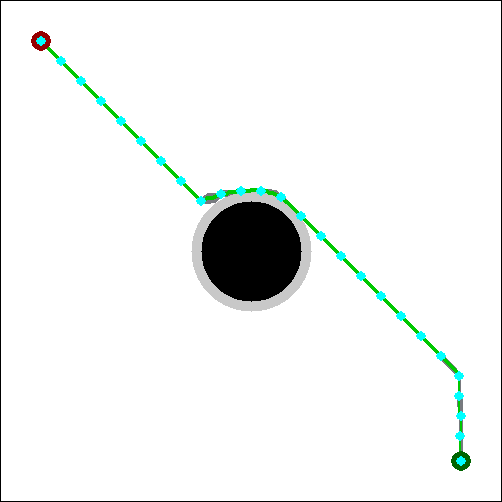
\includegraphics[width=\linewidth]{images/screenshot_51.png}
    \caption{Global Way-point LSTM Planner}
  \end{subfigure}
  \hfill
  \begin{subfigure}[b]{0.48\linewidth}
    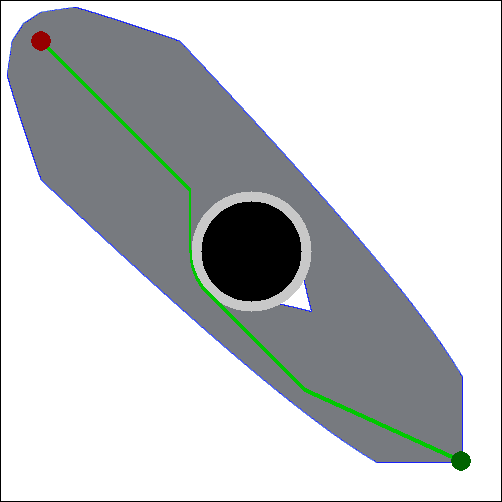
\includegraphics[width=\linewidth]{images/screenshot_44.png}
    \caption{A*}
  \end{subfigure}
  \newline
  \begin{subfigure}[b]{0.48\linewidth}
    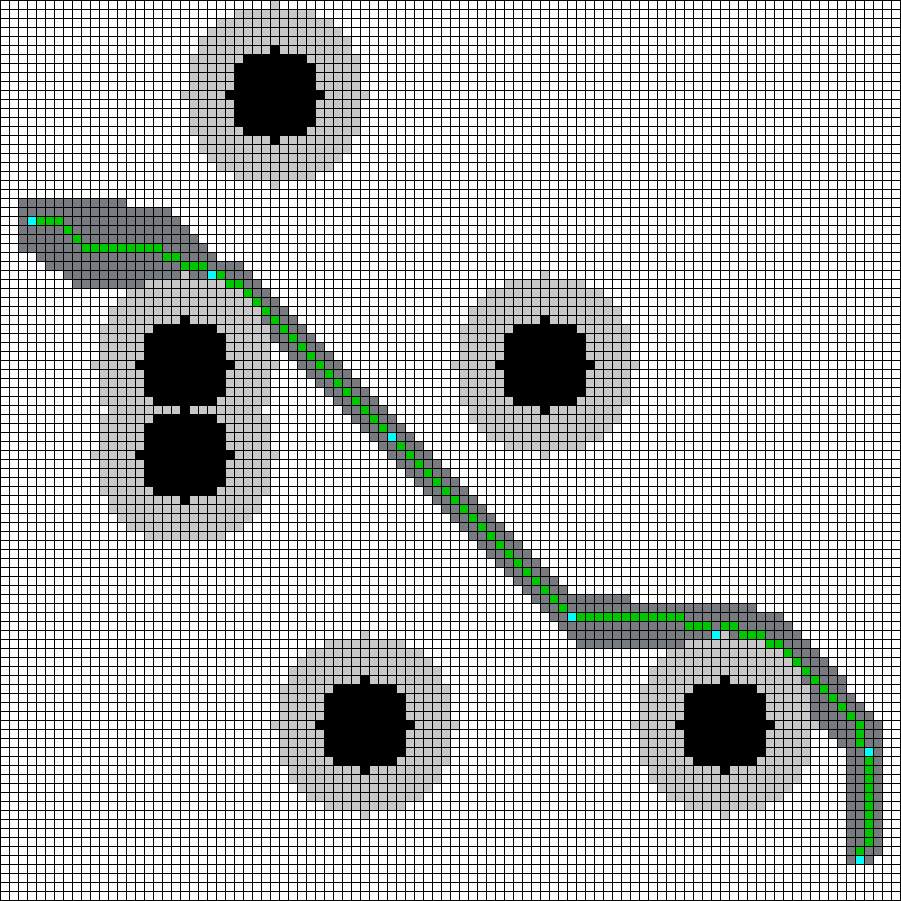
\includegraphics[width=\linewidth]{images/screenshot_104.png}
    \caption{Global Way-point LSTM Planner}
  \end{subfigure}
  \hfill
  \begin{subfigure}[b]{0.48\linewidth}
    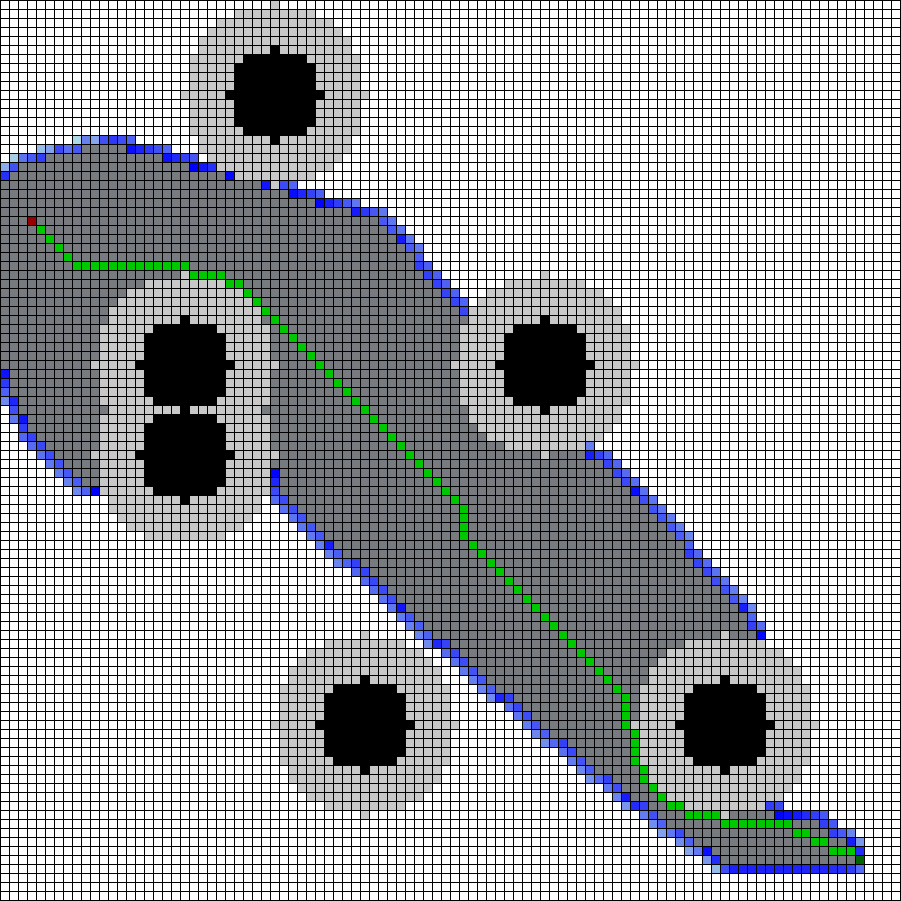
\includegraphics[width=\linewidth]{images/screenshot_105.png}
    \caption{A*}
  \end{subfigure}
  \caption{Global Way-point LSTM Planner and A* examples which showcase the memory/optimal distance trade-off}
  \label{fig: comparison_a*_waypoint}
\end{figure}

\pagebreak

\newpage

\section{Path Planning on Real-world Maps}

We have collected three real-world occupancy grid maps produced by SLAM sensors and converted them into internal maps. The maps have been used in the following works: \cite{first_map}, \cite{second_map} and \cite{third_map}.

Figures \ref{fig: wp_vs_a_1}, \ref{fig: wp_vs_a_2} and \ref{fig: wp_vs_a_3} highlight the performance of the Global Way-point LSTM Planner against A* on the real-world maps. Some runs achieve great results while others completely fail (in the sense that we fail to place the last global way-point on the goal). Furthermore, we can notice that the algorithm maintains the same behaviour across different environments which confirms the robustness to unknown environments property. This is intuitively correct, as we have used Machine Learning methods to find the path, and thus, we inherit the generalisation properties.

It should be noted that the run-times where significantly higher for the Global Way-point LSTM Planner due to the parallelising issue. We have also varied the global kernel max iterations to highlight the importance of choosing a proper argument. As a general rule, the number of iterations should be proportional to the size of the map.

\pagebreak

\begin{figure}[]
  \centering
  \begin{subfigure}[b]{0.48\linewidth}
    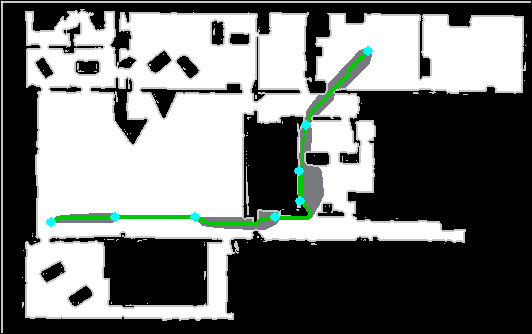
\includegraphics[width=\linewidth]{images/screenshot_134.png}
     \caption{Global Way-point LSTM Planner (max iterations 80)}
  \end{subfigure}
  \hfill
  \begin{subfigure}[b]{0.48\linewidth}
    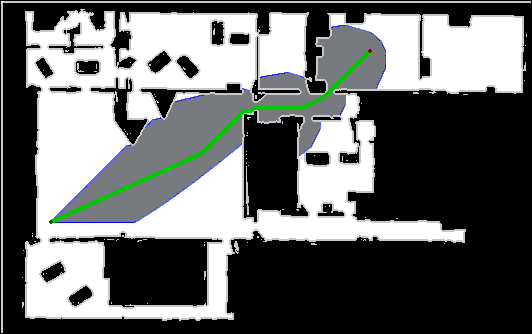
\includegraphics[width=\linewidth]{images/screenshot_107.png}
     \caption{A*\newline}
  \end{subfigure}
  \hfill
  \begin{subfigure}[b]{0.48\linewidth}
    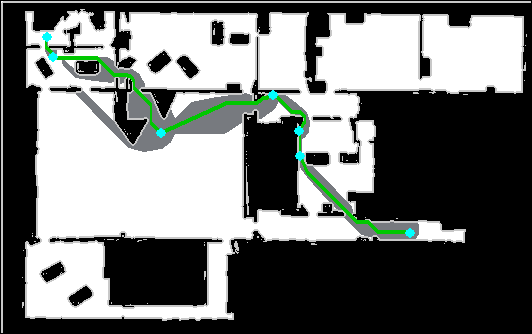
\includegraphics[width=\linewidth]{images/screenshot_137.png}
     \caption{Global Way-point LSTM Planner (max iterations 100)}
  \end{subfigure}
  \hfill
  \begin{subfigure}[b]{0.48\linewidth}
    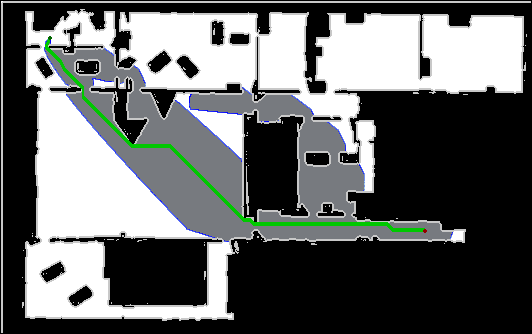
\includegraphics[width=\linewidth]{images/screenshot_109.png}
     \caption{A*\newline}
  \end{subfigure}
  \hfill
  \begin{subfigure}[b]{0.48\linewidth}
    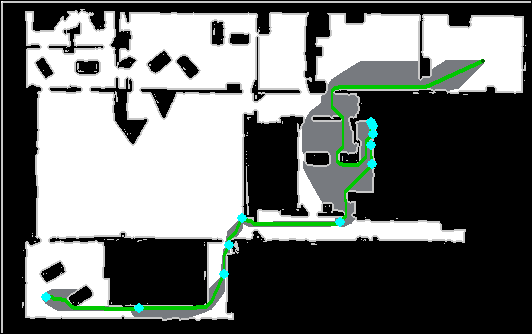
\includegraphics[width=\linewidth]{images/screenshot_138.png}
     \caption{Global Way-point LSTM Planner (max iterations 100)}
  \end{subfigure}
  \hfill
  \begin{subfigure}[b]{0.48\linewidth}
    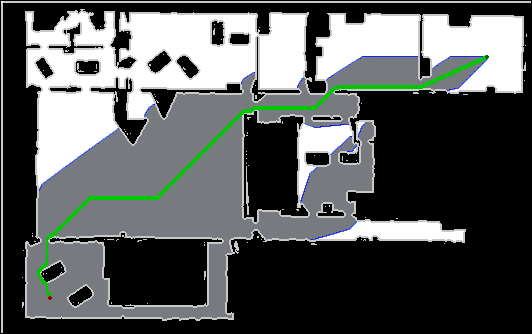
\includegraphics[width=\linewidth]{images/screenshot_110.png}
     \caption{A*\newline}
  \end{subfigure}
  \hfill
  \begin{subfigure}[b]{0.48\linewidth}
    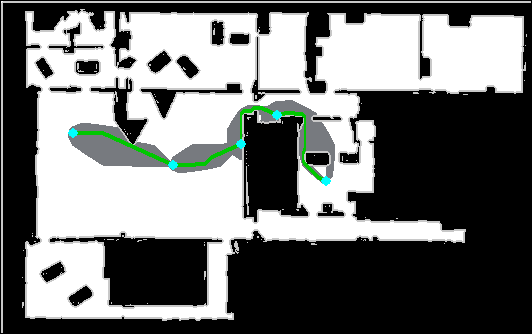
\includegraphics[width=\linewidth]{images/screenshot_140.png}
     \caption{Global Way-point LSTM Planner (max iterations 100)}
  \end{subfigure}
  \hfill
  \begin{subfigure}[b]{0.48\linewidth}
    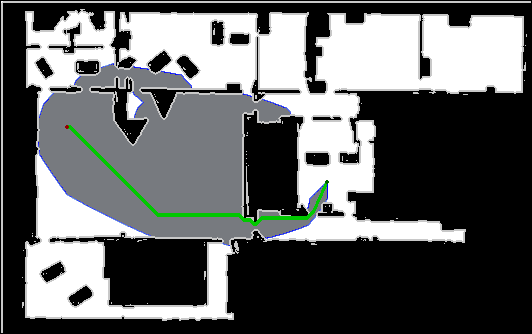
\includegraphics[width=\linewidth]{images/screenshot_114.png}
     \caption{A*\newline}
  \end{subfigure}
  \caption{Global Way-point LSTM Planner vs A* runs on real-world occupancy grid maps \cite{first_map}}
  \label{fig: wp_vs_a_1}
\end{figure}

\begin{figure}[]
  \centering
  \begin{subfigure}[b]{0.38\linewidth}
    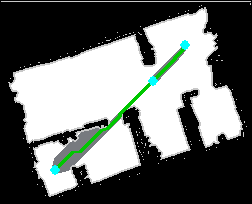
\includegraphics[width=\linewidth]{images/screenshot_141.png}
     \caption{Global Way-point LSTM Planner (max iterations 100)}
  \end{subfigure}
  \hfill
  \begin{subfigure}[b]{0.38\linewidth}
    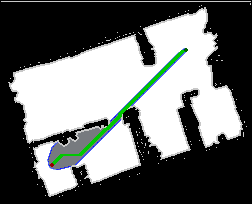
\includegraphics[width=\linewidth]{images/screenshot_116.png}
     \caption{A*\newline}
  \end{subfigure}
  \newline
  \begin{subfigure}[b]{0.38\linewidth}
    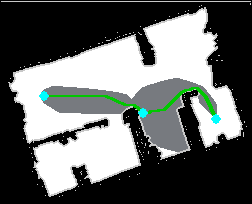
\includegraphics[width=\linewidth]{images/screenshot_142.png}
     \caption{Global Way-point LSTM Planner (max iterations 100)}
  \end{subfigure}
  \hfill
  \begin{subfigure}[b]{0.38\linewidth}
    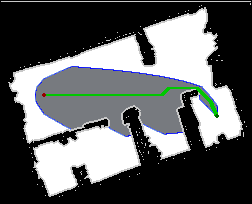
\includegraphics[width=\linewidth]{images/screenshot_117.png}
     \caption{A*\newline}
  \end{subfigure}
  \newline
  \begin{subfigure}[b]{0.38\linewidth}
    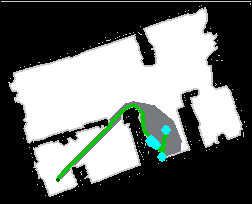
\includegraphics[width=\linewidth]{images/screenshot_143.png}
     \caption{Global Way-point LSTM Planner (max iterations 100)}
  \end{subfigure}
  \hfill
  \begin{subfigure}[b]{0.38\linewidth}
    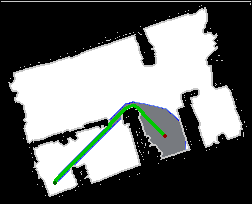
\includegraphics[width=\linewidth]{images/screenshot_118.png}
     \caption{A*\newline}
  \end{subfigure}
  \newline
  \begin{subfigure}[b]{0.38\linewidth}
    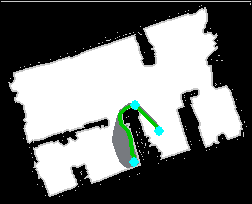
\includegraphics[width=\linewidth]{images/screenshot_147.png}
     \caption{Global Way-point LSTM Planner (max iterations 100)}
  \end{subfigure}
  \hfill
  \begin{subfigure}[b]{0.38\linewidth}
    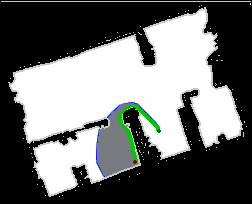
\includegraphics[width=\linewidth]{images/screenshot_146.png}
     \caption{A*\newline}
  \end{subfigure}
  \caption{Global Way-point LSTM Planner vs A* runs on real-world occupancy grid maps \cite{second_map}}
  \label{fig: wp_vs_a_2}
\end{figure}

\begin{figure}[]
  \centering
  \begin{subfigure}[b]{0.40\linewidth}
    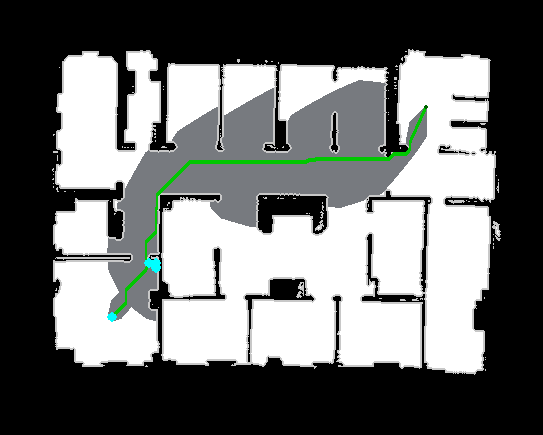
\includegraphics[width=\linewidth]{images/screenshot_144.png}
     \caption{Global Way-point LSTM Planner (max iterations 100)}
  \end{subfigure}
  \hfill
  \begin{subfigure}[b]{0.40\linewidth}
    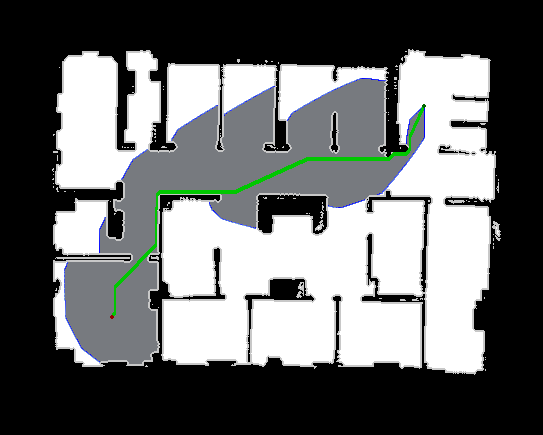
\includegraphics[width=\linewidth]{images/screenshot_124.png}
     \caption{A*\newline}
  \end{subfigure}
  \hfill
  \begin{subfigure}[b]{0.40\linewidth}
    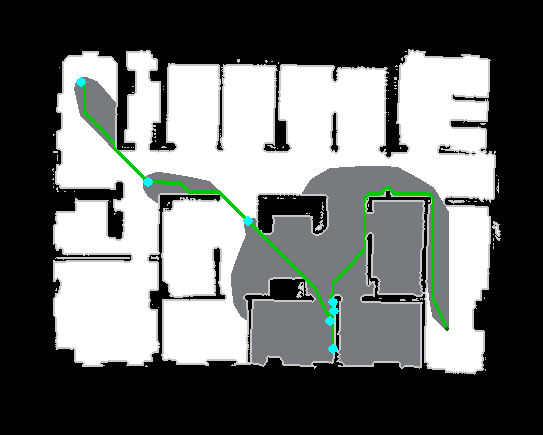
\includegraphics[width=\linewidth]{images/screenshot_148.png}
     \caption{Global Way-point LSTM Planner (max iterations 100)}
  \end{subfigure}
  \hfill
  \begin{subfigure}[b]{0.40\linewidth}
    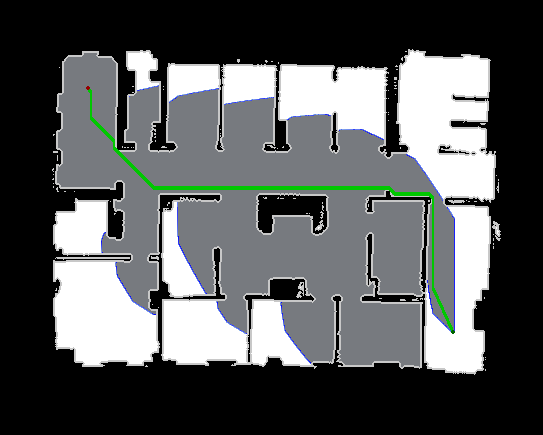
\includegraphics[width=\linewidth]{images/screenshot_125.png}
     \caption{A*\newline}
  \end{subfigure}
  \hfill
  \begin{subfigure}[b]{0.40\linewidth}
    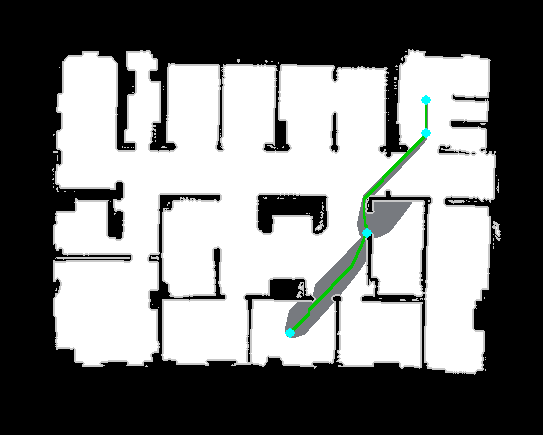
\includegraphics[width=\linewidth]{images/screenshot_149.png}
     \caption{Global Way-point LSTM Planner (max iterations 100)}
  \end{subfigure}
  \hfill
  \begin{subfigure}[b]{0.40\linewidth}
    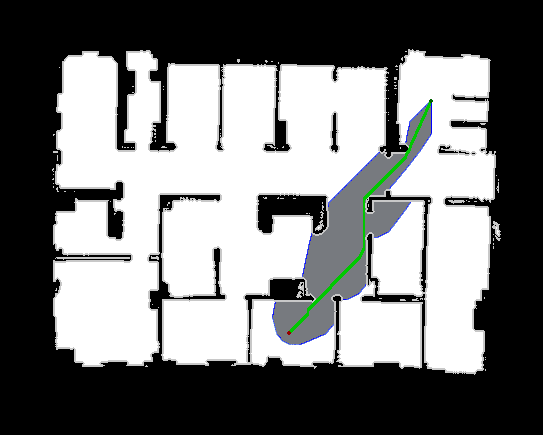
\includegraphics[width=\linewidth]{images/screenshot_126.png}
     \caption{A*\newline}
  \end{subfigure}
  \hfill
  \begin{subfigure}[b]{0.40\linewidth}
    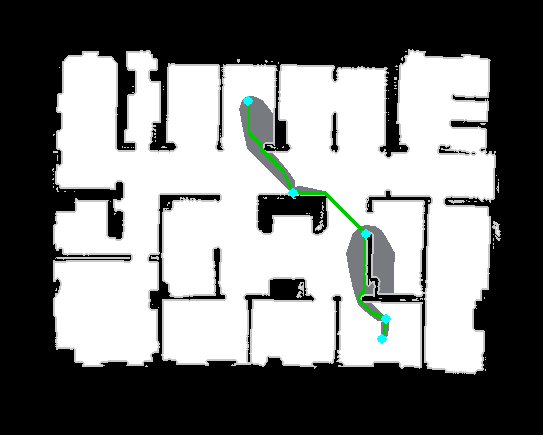
\includegraphics[width=\linewidth]{images/screenshot_150.png}
     \caption{Global Way-point LSTM Planner (max iterations 100)}
  \end{subfigure}
  \hfill
  \begin{subfigure}[b]{0.40\linewidth}
    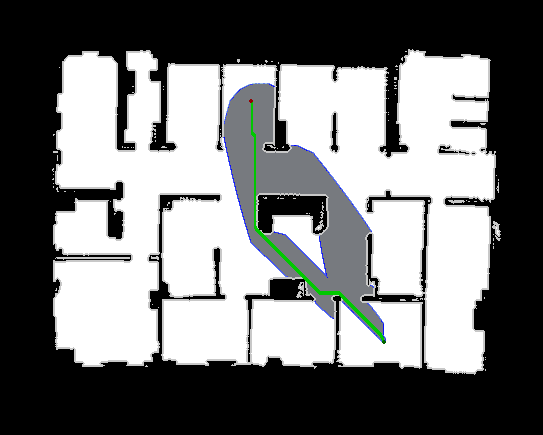
\includegraphics[width=\linewidth]{images/screenshot_127.png}
     \caption{A*\newline}
  \end{subfigure}
  \caption{Global Way-point LSTM Planner vs A* runs on real-world occupancy grid maps \cite{third_map}}
  \label{fig: wp_vs_a_3}
\end{figure}

\FloatBarrier

\section{Path Planning on Real-world Robot}
\label{sec: robotexp}

The final evaluation will be run on a real-world robot at Imperial College London (See Figure \ref{fig: robot}). We will use a basic 4-wheeler robot with a YDLidar sensor attached at the top. The YDLidar sensor is a 360-degree two-dimensional distance measurement device which produces a SLAM output image scan \cite{ydlidar}. The robot (Perceptbot) was build as a novel development platform for robotics by a group of students \cite{robo}. The robot has support for multiple hardware attachments (such as an external camera and an Intel Neural Compute Stick for Machine Learning), but we have only used the YDLidar sensor. The motherboard of the robot is a Raspberry Pi circuit board \cite{Halfacree:2012:RPU:2432381} which is running \textit{Raspbian} \cite{raspbian}, and makes use of the \textit{ROS} library for motion controlling.

\begin{figure}[h!]
  \centering
  \begin{subfigure}[b]{0.47\linewidth}
    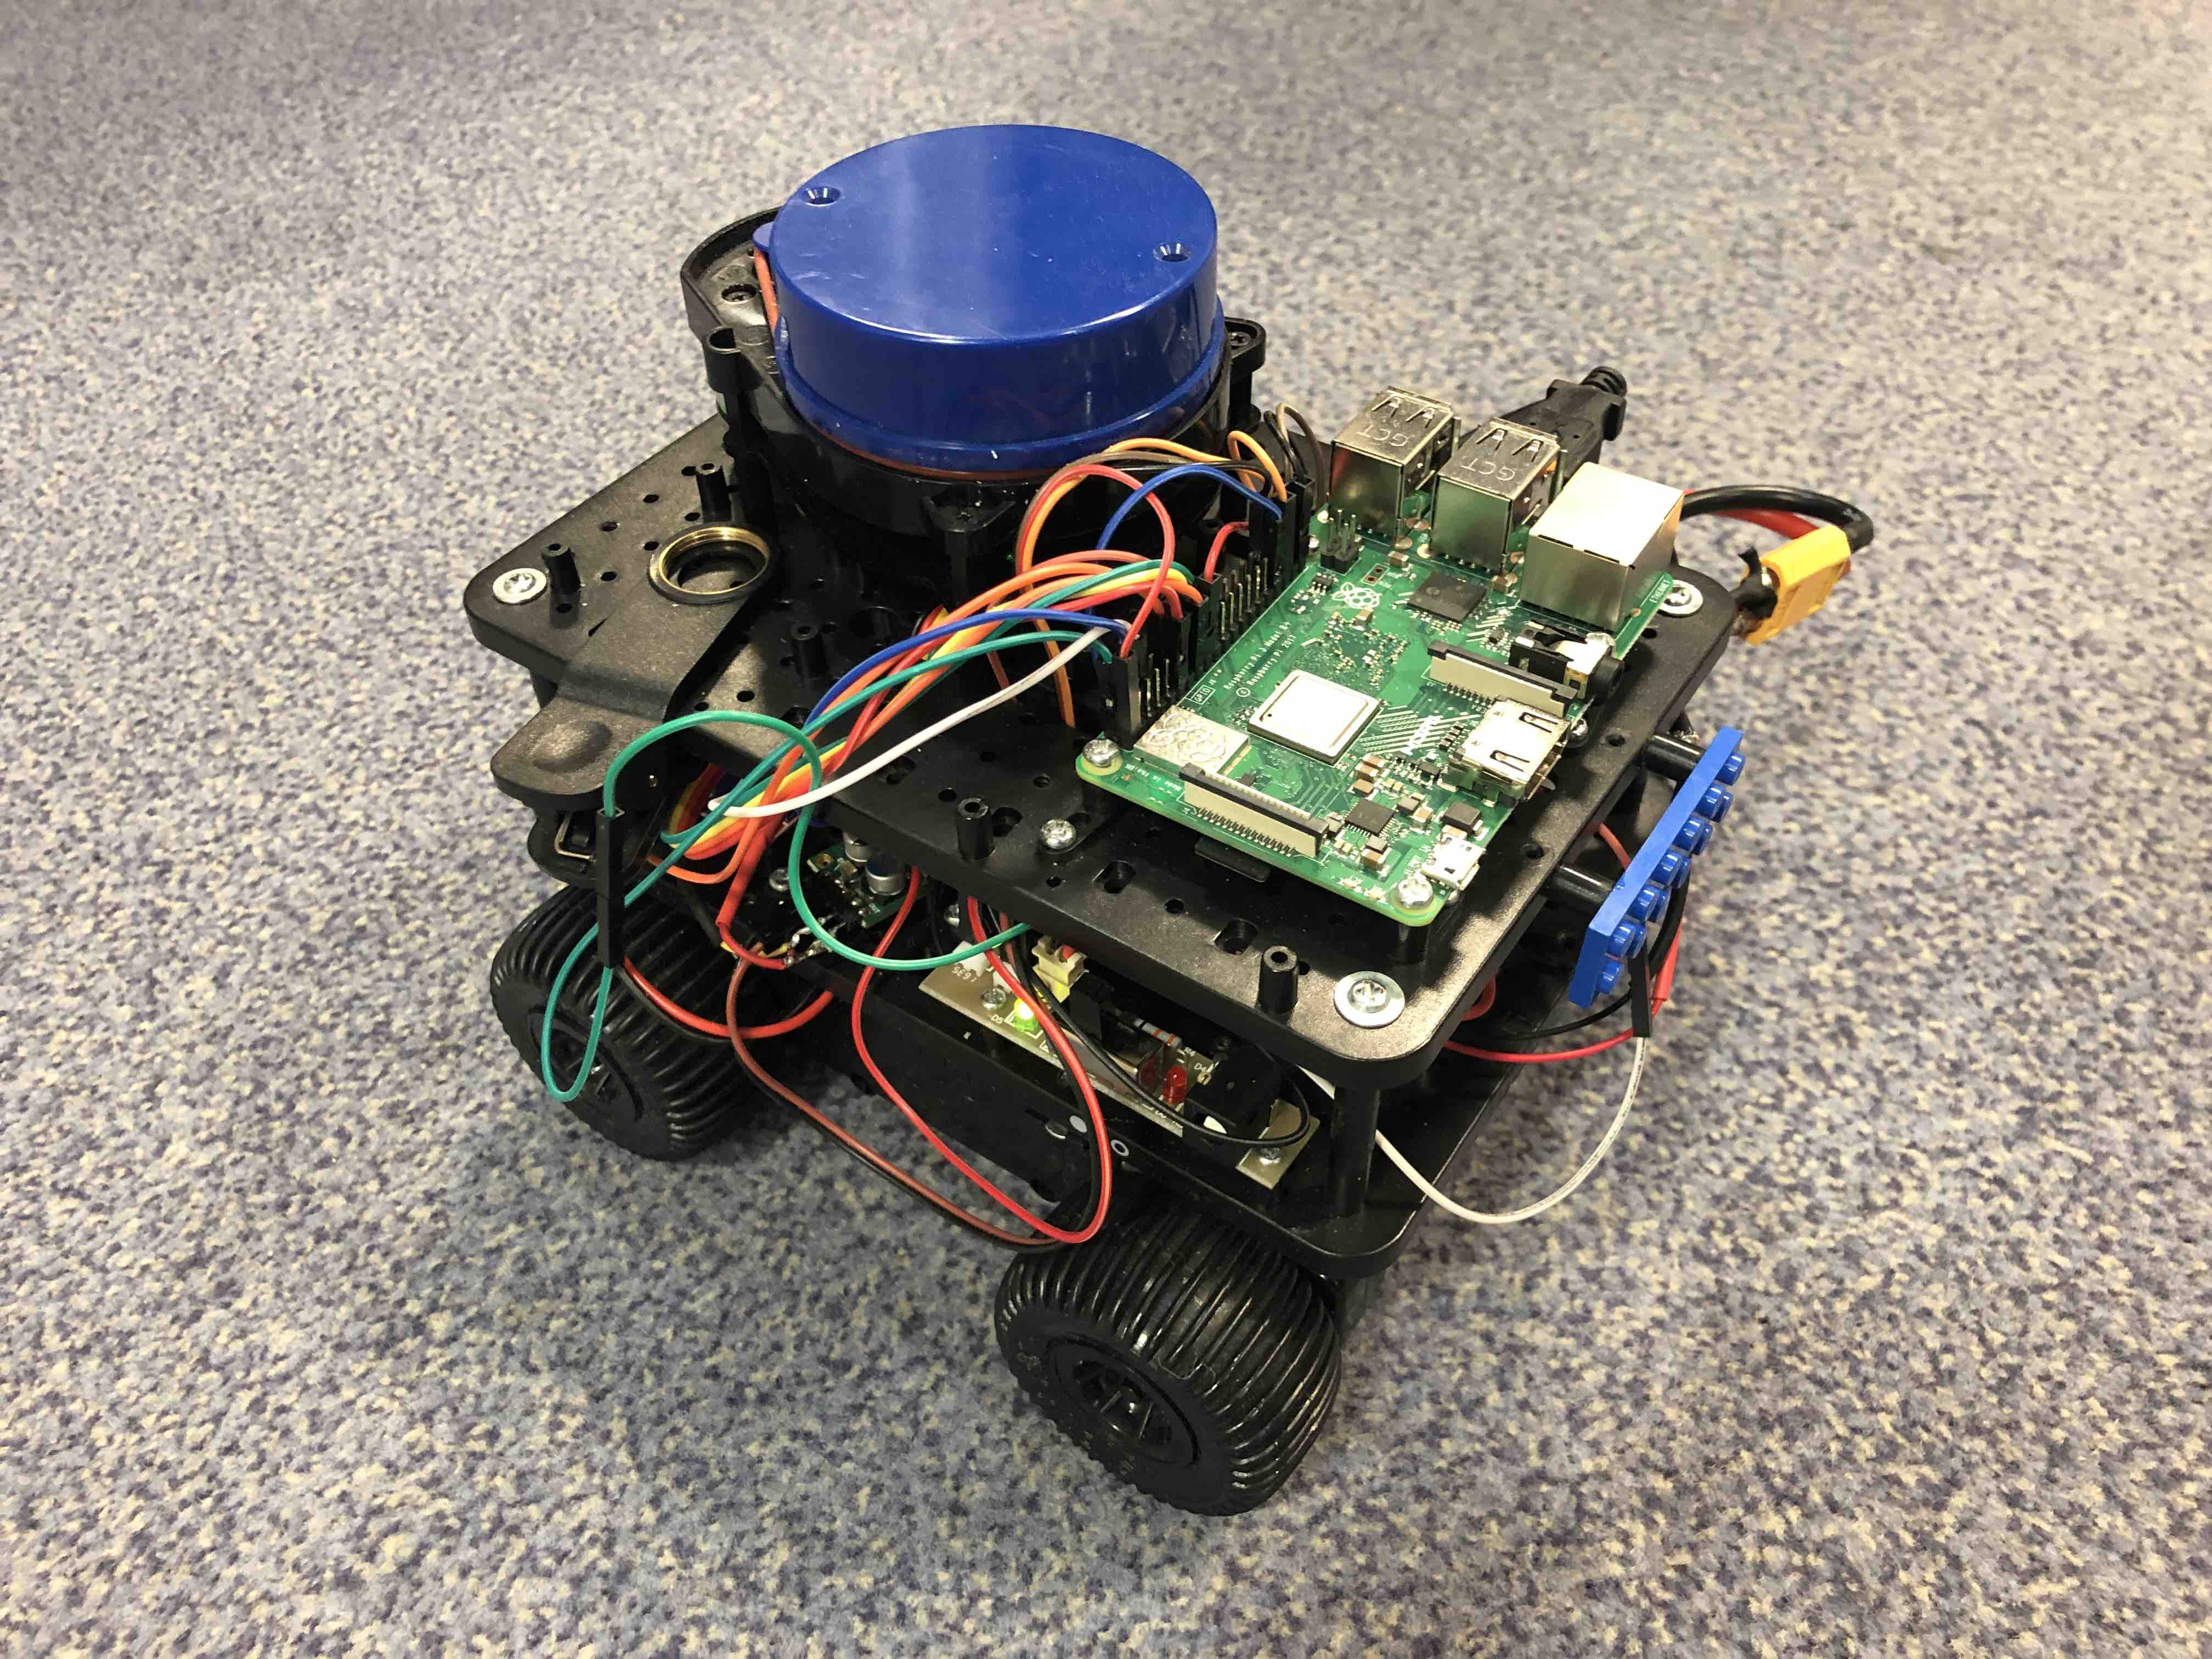
\includegraphics[width=\linewidth]{images/real/robo/preview.JPG}
     \caption{Robot (Perceptbot) with YDLidar Sensor \cite{robo}}
  \end{subfigure}
  \hfill
  \begin{subfigure}[b]{0.47\linewidth}
    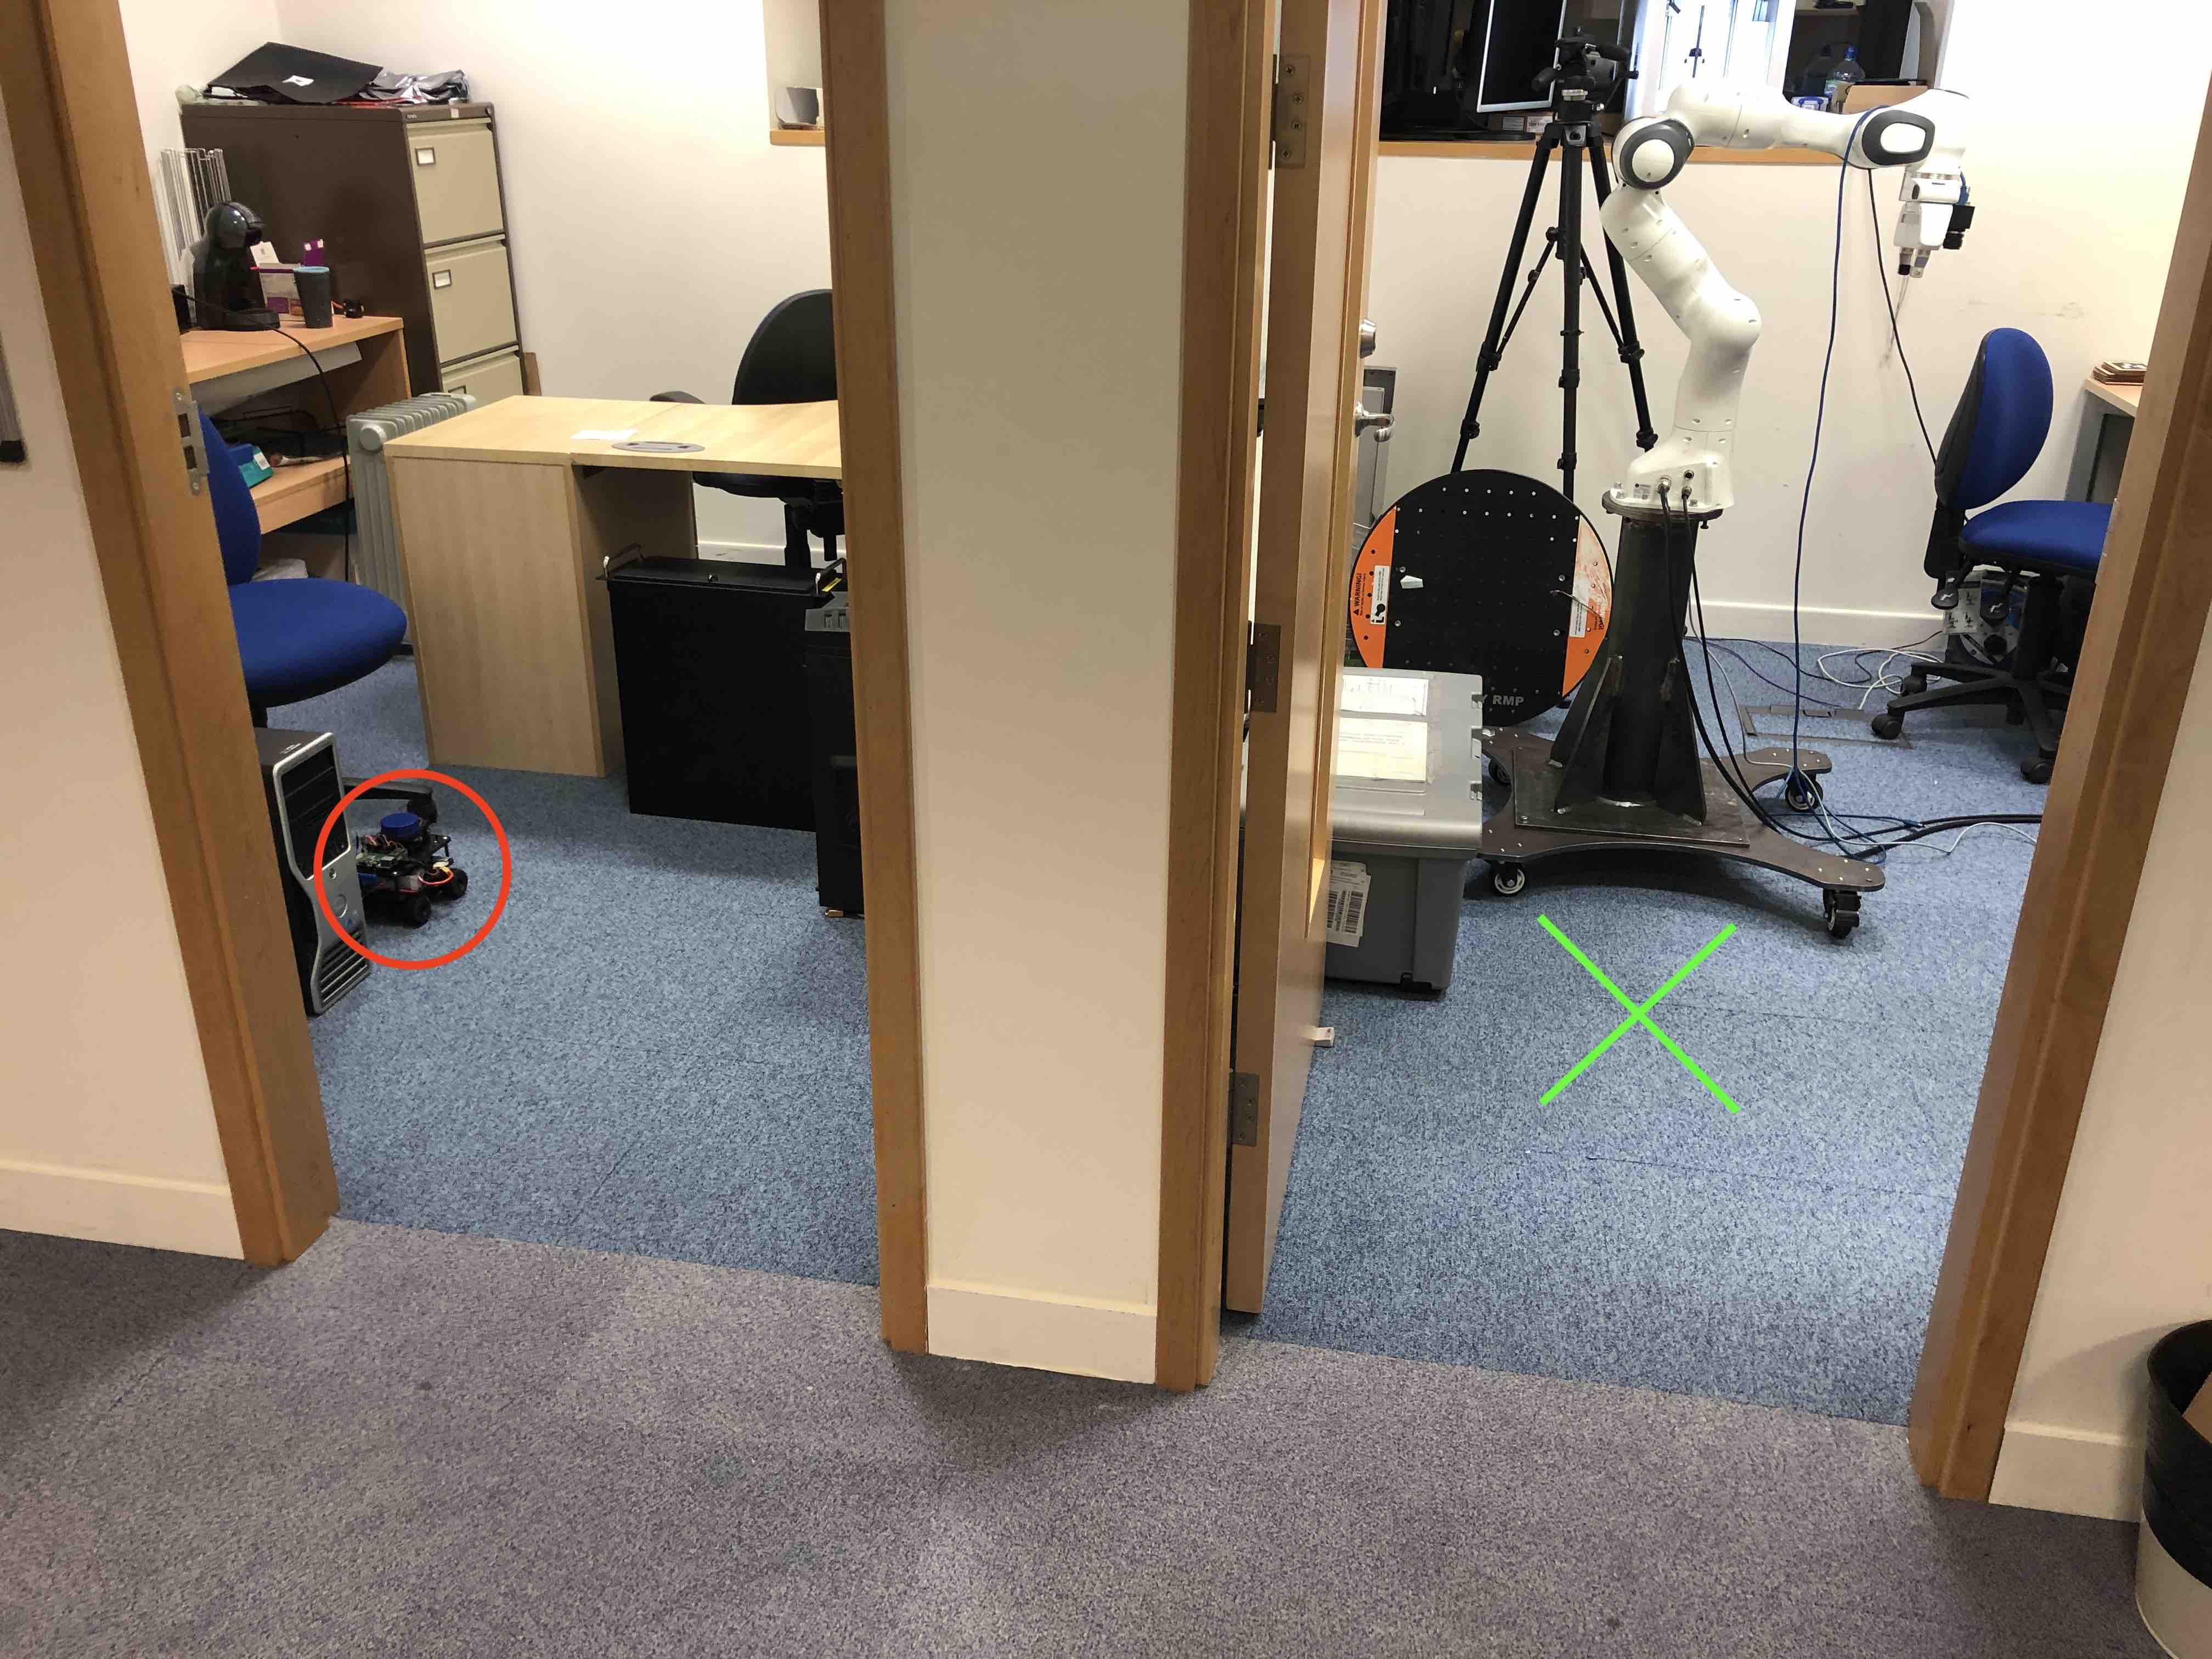
\includegraphics[width=\linewidth]{images/real/robo/start_ann.JPG}
     \caption{Planned trajectory: start and goal positions}
  \end{subfigure}
  \caption{The robot (Perceptbot) (a) and the planned trajectory (b). The red circle represents the robot position (agent) and the green \xmark $\,$ represents the desired destination (goal)}
  \label{fig: robot}
\end{figure}

We have created a \textit{ROS} master node (\textbf{Ros} component) which contains the Global Way-point LSTM Planner and a Motion Planner. The Motion Planner is responsible for physically moving the robot to the specified goal (or way-point), by querying simple velocity control commands using the \textit{cmd\_vel} \textit{ROS} package, and for converting the real world coordinates into PathBench \textbf{Simulator} coordinates and vice-versa. The agent position and rotation is retrieved using the \textit{robot\_pose} \textit{ROS} \textit{package}. The YDLidar sensor is run using the \textit{gmapping} \textit{ROS} package with 0.15 meters grid cell size. Lastly, we have run the \textbf{Ros} master node and \textit{gmapping} on a server which uses network packets (i.e. \textit{ROS} publisher-subscriber APIs) to communicate with the robot. This was done because the performance of the \textit{gmapping} package was severely impacted by the hardware limitations of the Raspberry Pi. The \textbf{Ros} master node could have been run on the Raspberry Pi itself, but we have configured it on the server for faster development and debugging. The \textit{gmapping} SLAM scan output was integrated into PathBench by creating a custom map environment (\textbf{RosMap}), which has support for live updates.

The algorithm starts by converting all trace points generated by the Global Way-point LSTM Planner, including the ones generated by the local kernel, into way-points. The planning between two way-points is achieved by the Motion Planner with simple velocity commands. In the first phase, we rotate the robot so that the robot angle is equal to the angle of the direction to the next way-point. In the second phase, we move in a straight line until we reach the next way-point. If at any point we surpass a pre-defined angle threshold, we correct the robot pose by executing the first phase again, and continue the process. We only request a map update when we have reached the way-points suggested by the global kernel as the local kernel (A*) is offline (See Figure \ref{fig: robot_motion} and Algorithm \ref{alg: real_robot}).

Figure \ref{fig: robot_run} showcases the performance of the real robot on the trajectory defined in Figure \ref{fig: robot}. We will also place the side by side view of the PathBench \textbf{Simulator} and the \textit{ROS} simulator, Rviz. Table \ref{tab: robot_stats} contains the evaluation results reported by our platform.

\pagebreak

\begin{figure}[h!]
  \centering
  \begin{subfigure}[b]{0.4\linewidth}
    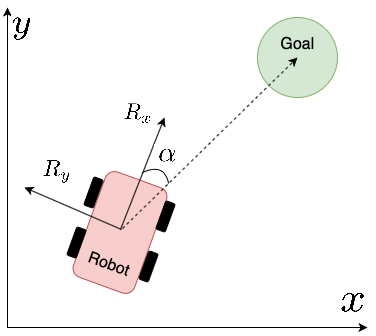
\includegraphics[width=\linewidth]{images/robot.png}
     \caption{First Phase: Rotation}
  \end{subfigure}
  \hfill
  \begin{subfigure}[b]{0.4\linewidth}
    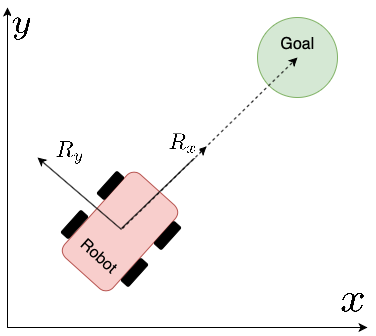
\includegraphics[width=\linewidth]{images/robot_2.png}
     \caption{Second Phase: Forward Movement}
  \end{subfigure}
  \caption{The illustrated two phases of the motion planning between two way-points. $x$ and $y$ are the world coordinate system and $R_x$ and $R_y$ are the robot frame coordinate system}
  \label{fig: robot_motion}
\end{figure}

\begin{algorithm}[h!]
\caption{Robot-Planner}
\label{alg: real_robot}
\begin{algorithmic}[1]

\Procedure{Motion-Planner}{$wp$, $max\_it$, $angle\_threshold$, $goal\_threshold$}
    \For{$i$ in [0, $max\_it$)}
        \State $agent\_pos \gets$ query agent position
        \State $agent\_angle \gets$ query agent angle relative to the world coordinate system
        \State $goal\_dir \gets$ $wp$ - $agent\_pos$
        \State $goal\_angle \gets$ \texttt{arctan2}($goal\_dir.y$, $goal\_dir.x$)
        \State $\alpha \gets$ \texttt{sign}($goal\_angle - agent\_angle$) ($|goal\_angle - agent\_angle|$ \% $\pi$)
        \State
        \If {$\alpha \geq angle\_threshold$}
            \State rotate with velocity proportional to $\alpha$
            \State \textbf{continue}
        \EndIf
        \State
        \If {$\norm{goal\_dir}_{2} \geq dist\_threshold$}
            \State move forward with velocity proportional to $\norm{goal\_dir}_{2}$
            \State \textbf{continue}
        \Else
            \State \textbf{return}
        \EndIf
    \EndFor
    \State
\EndProcedure

\Procedure{Robot-Planner}{$M\colon(A, Os, G)$}
    \While {goal is not reached}
        \State $M \gets$ query new SLAM scan
        \State $way\_points \gets$ get Global Way-point LSTM Planner trace until next global way-point
        \State
        \For {$wp$ in $way\_points$}
            \State \textit{Motion-Planner}($wp$, 1000, 0.1, 0.1)
        \EndFor
        \State
        \If {there are no $way\_points$}
            \State goal was not found
            \State \textbf{break}
        \EndIf
    \EndWhile
\EndProcedure
\end{algorithmic}
\end{algorithm}

\pagebreak

\begin{figure}[h!]
  \centering
  \begin{subfigure}[b]{0.32\linewidth}
    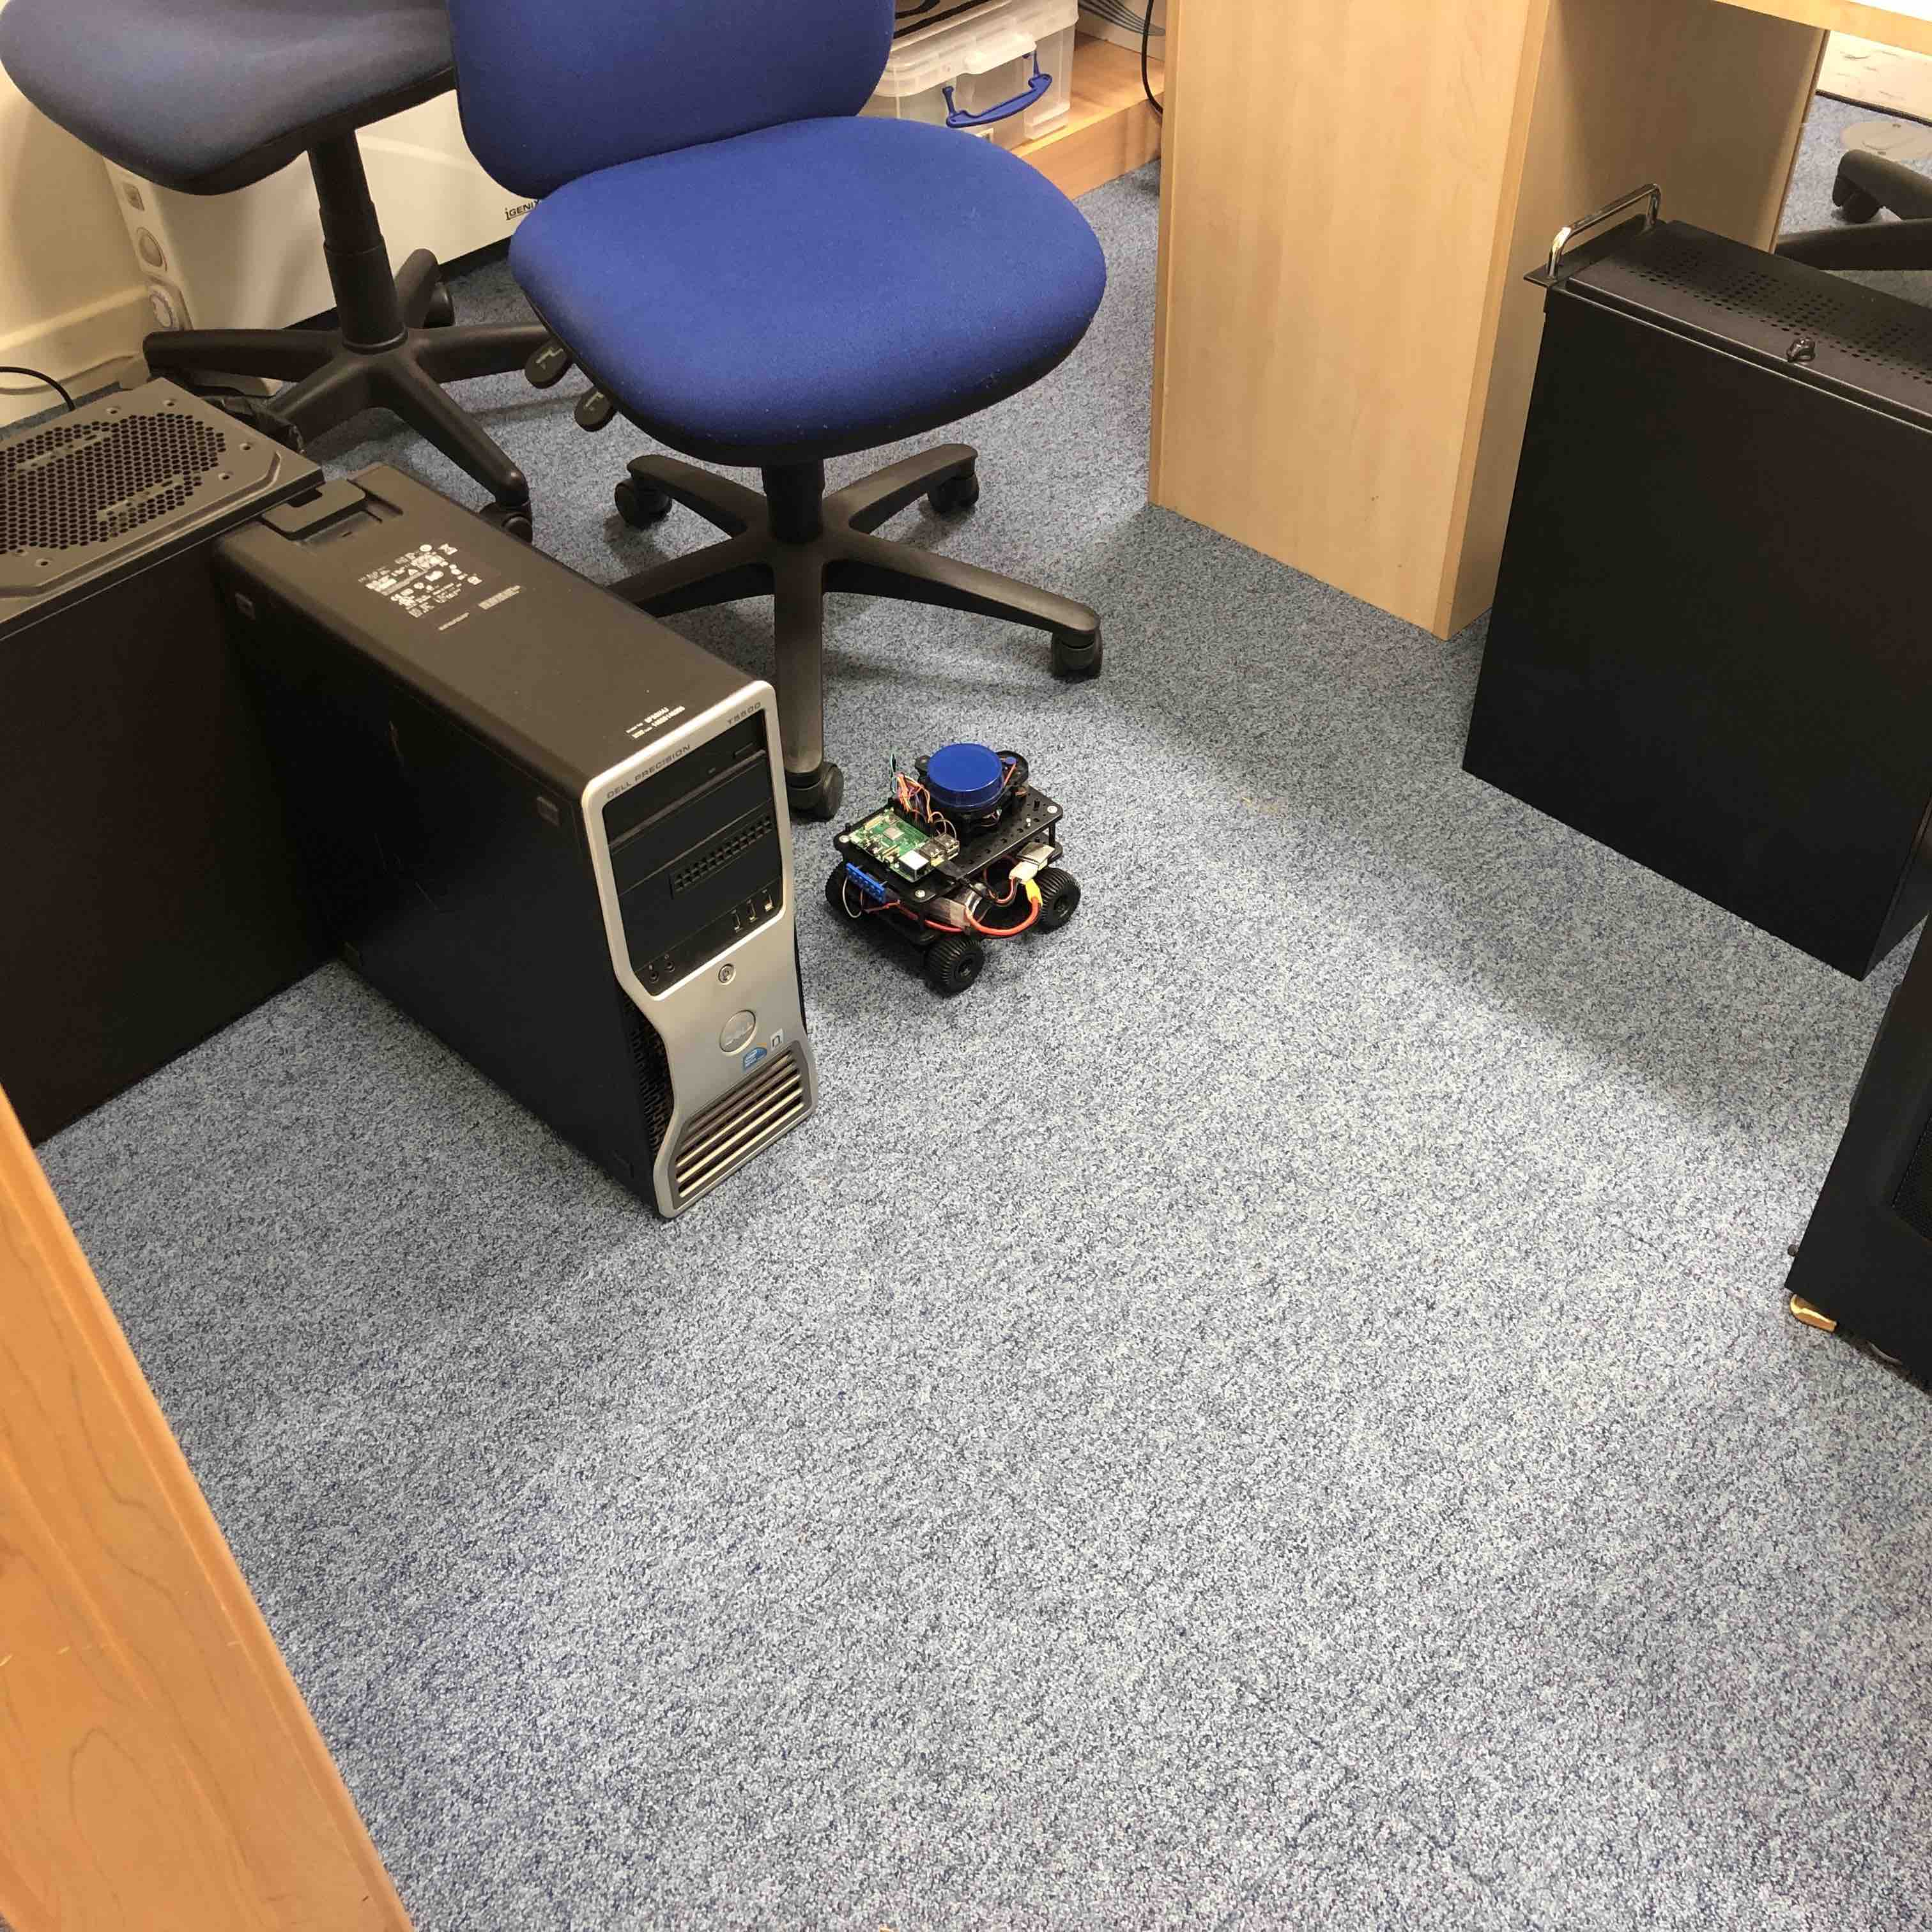
\includegraphics[width=\linewidth]{images/real/robo/start_2.JPG}
     \caption{Real-world: Start}
  \end{subfigure}
  \hfill
  \begin{subfigure}[b]{0.32\linewidth}
    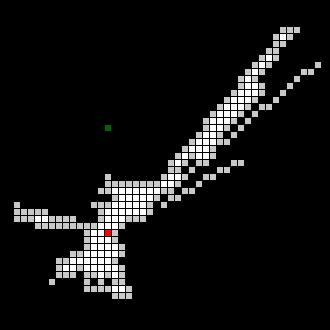
\includegraphics[width=\linewidth]{images/real/sys/start_2.png}
     \caption{PathBench: Start}
  \end{subfigure}
  \hfill
  \begin{subfigure}[b]{0.32\linewidth}
    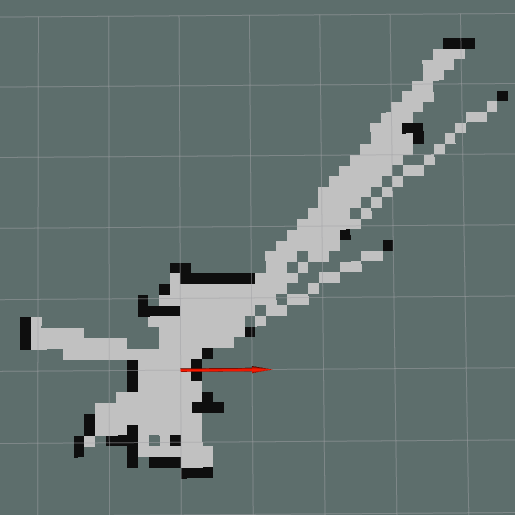
\includegraphics[width=\linewidth]{images/real/sys/start_3.png}
     \caption{Rviz: Start}
  \end{subfigure}
  
  \newline
  
  \begin{subfigure}[b]{0.32\linewidth}
    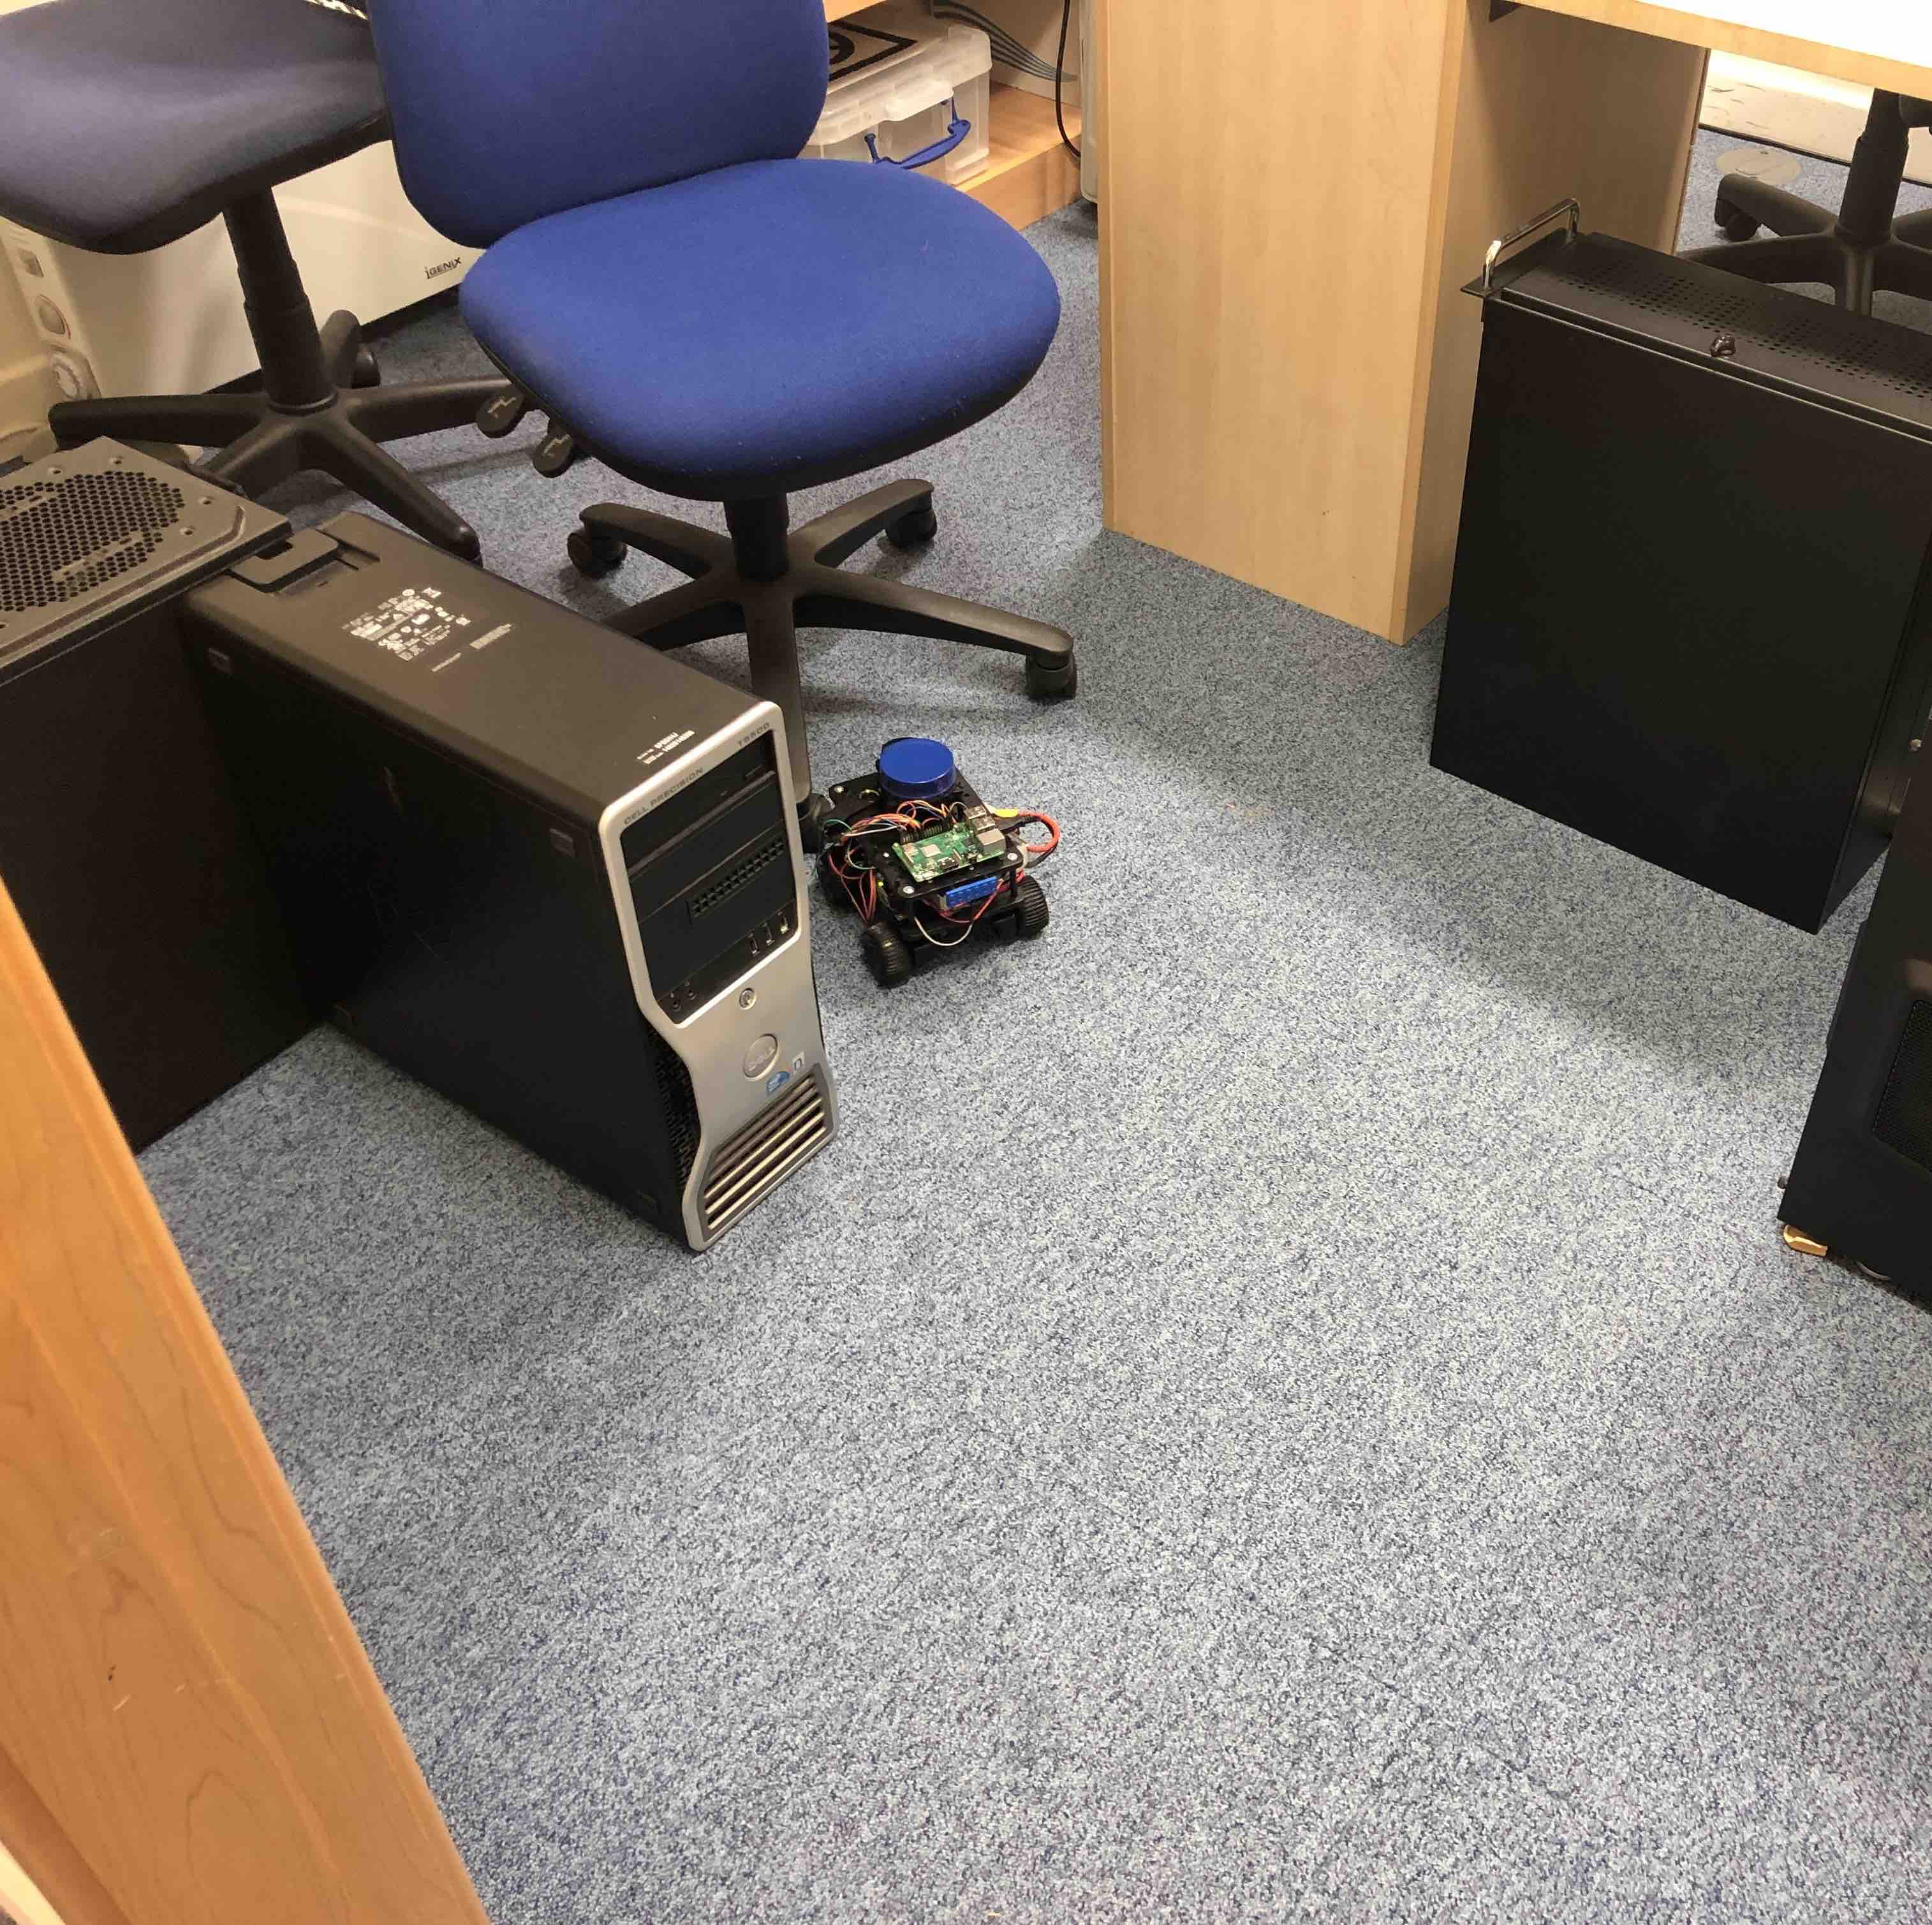
\includegraphics[width=\linewidth]{images/real/robo/1.JPG}
     \caption{Real-world: Suggested WP 1}
  \end{subfigure}
  \hfill
  \begin{subfigure}[b]{0.32\linewidth}
    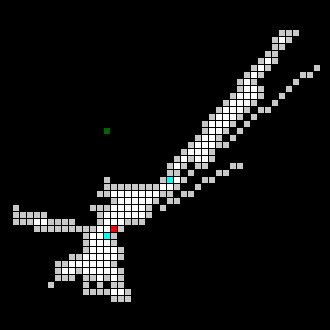
\includegraphics[width=\linewidth]{images/real/sys/1_2.png}
     \caption{PathBench: Suggested WP 1}
  \end{subfigure}
  \hfill
  \begin{subfigure}[b]{0.32\linewidth}
    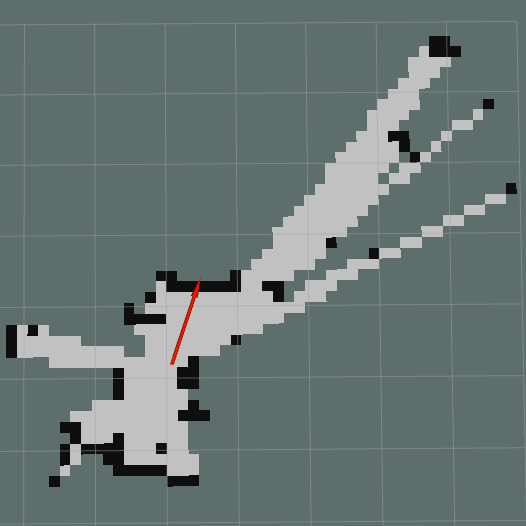
\includegraphics[width=\linewidth]{images/real/sys/1_3.png}
     \caption{Rviz: Suggested WP 1}
  \end{subfigure}
  
  \newline
  
  \begin{subfigure}[b]{0.32\linewidth}
    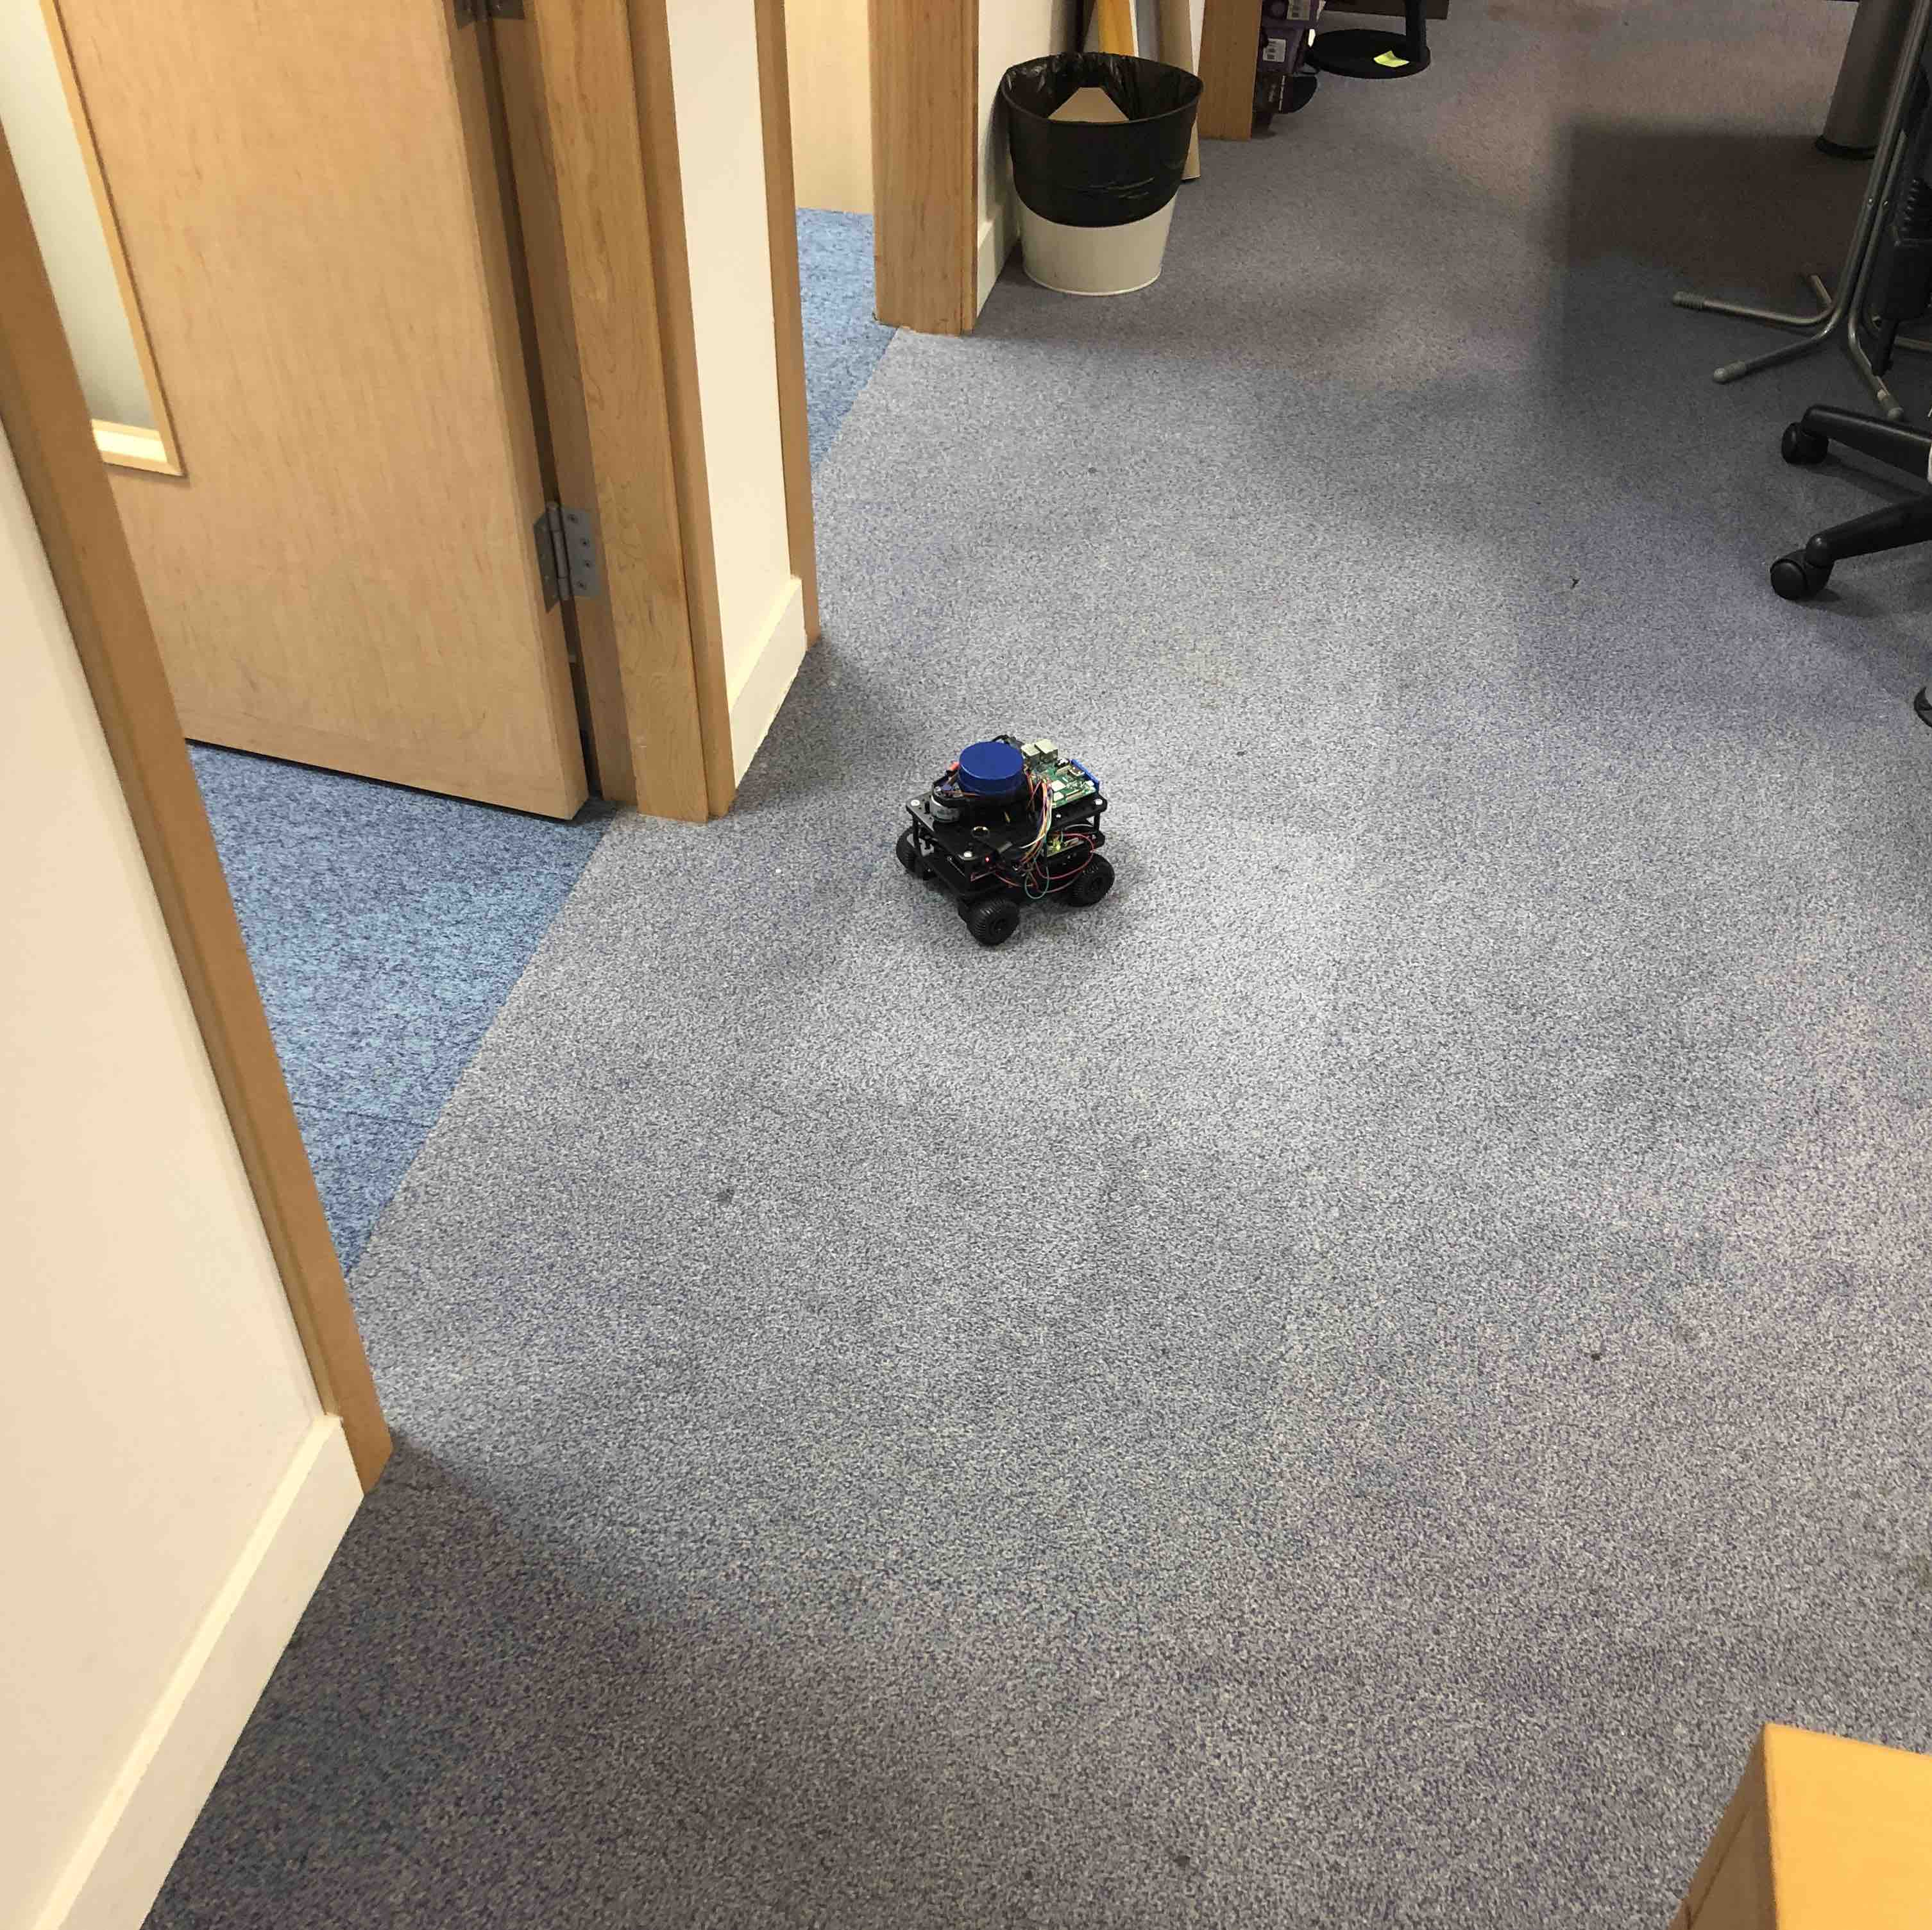
\includegraphics[width=\linewidth]{images/real/robo/2.JPG}
     \caption{Real-world: Reached WP 1}
  \end{subfigure}
  \hfill
  \begin{subfigure}[b]{0.32\linewidth}
    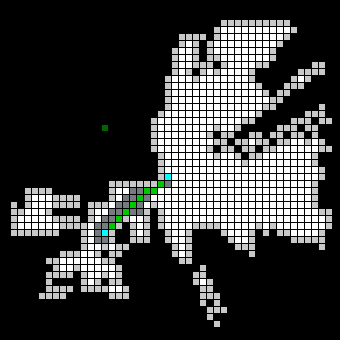
\includegraphics[width=\linewidth]{images/real/sys/2_2.png}
     \caption{PathBench: Reached WP 1}
  \end{subfigure}
  \hfill
  \begin{subfigure}[b]{0.32\linewidth}
    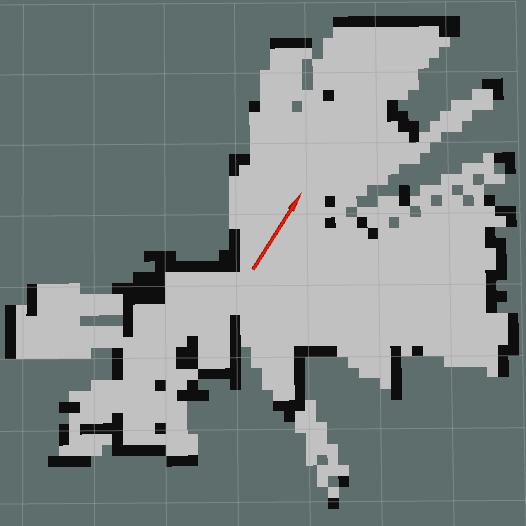
\includegraphics[width=\linewidth]{images/real/sys/2_3.png}
     \caption{Rviz: Reached WP 1}
  \end{subfigure}
  
  \newline
  
  \begin{subfigure}[b]{0.32\linewidth}
    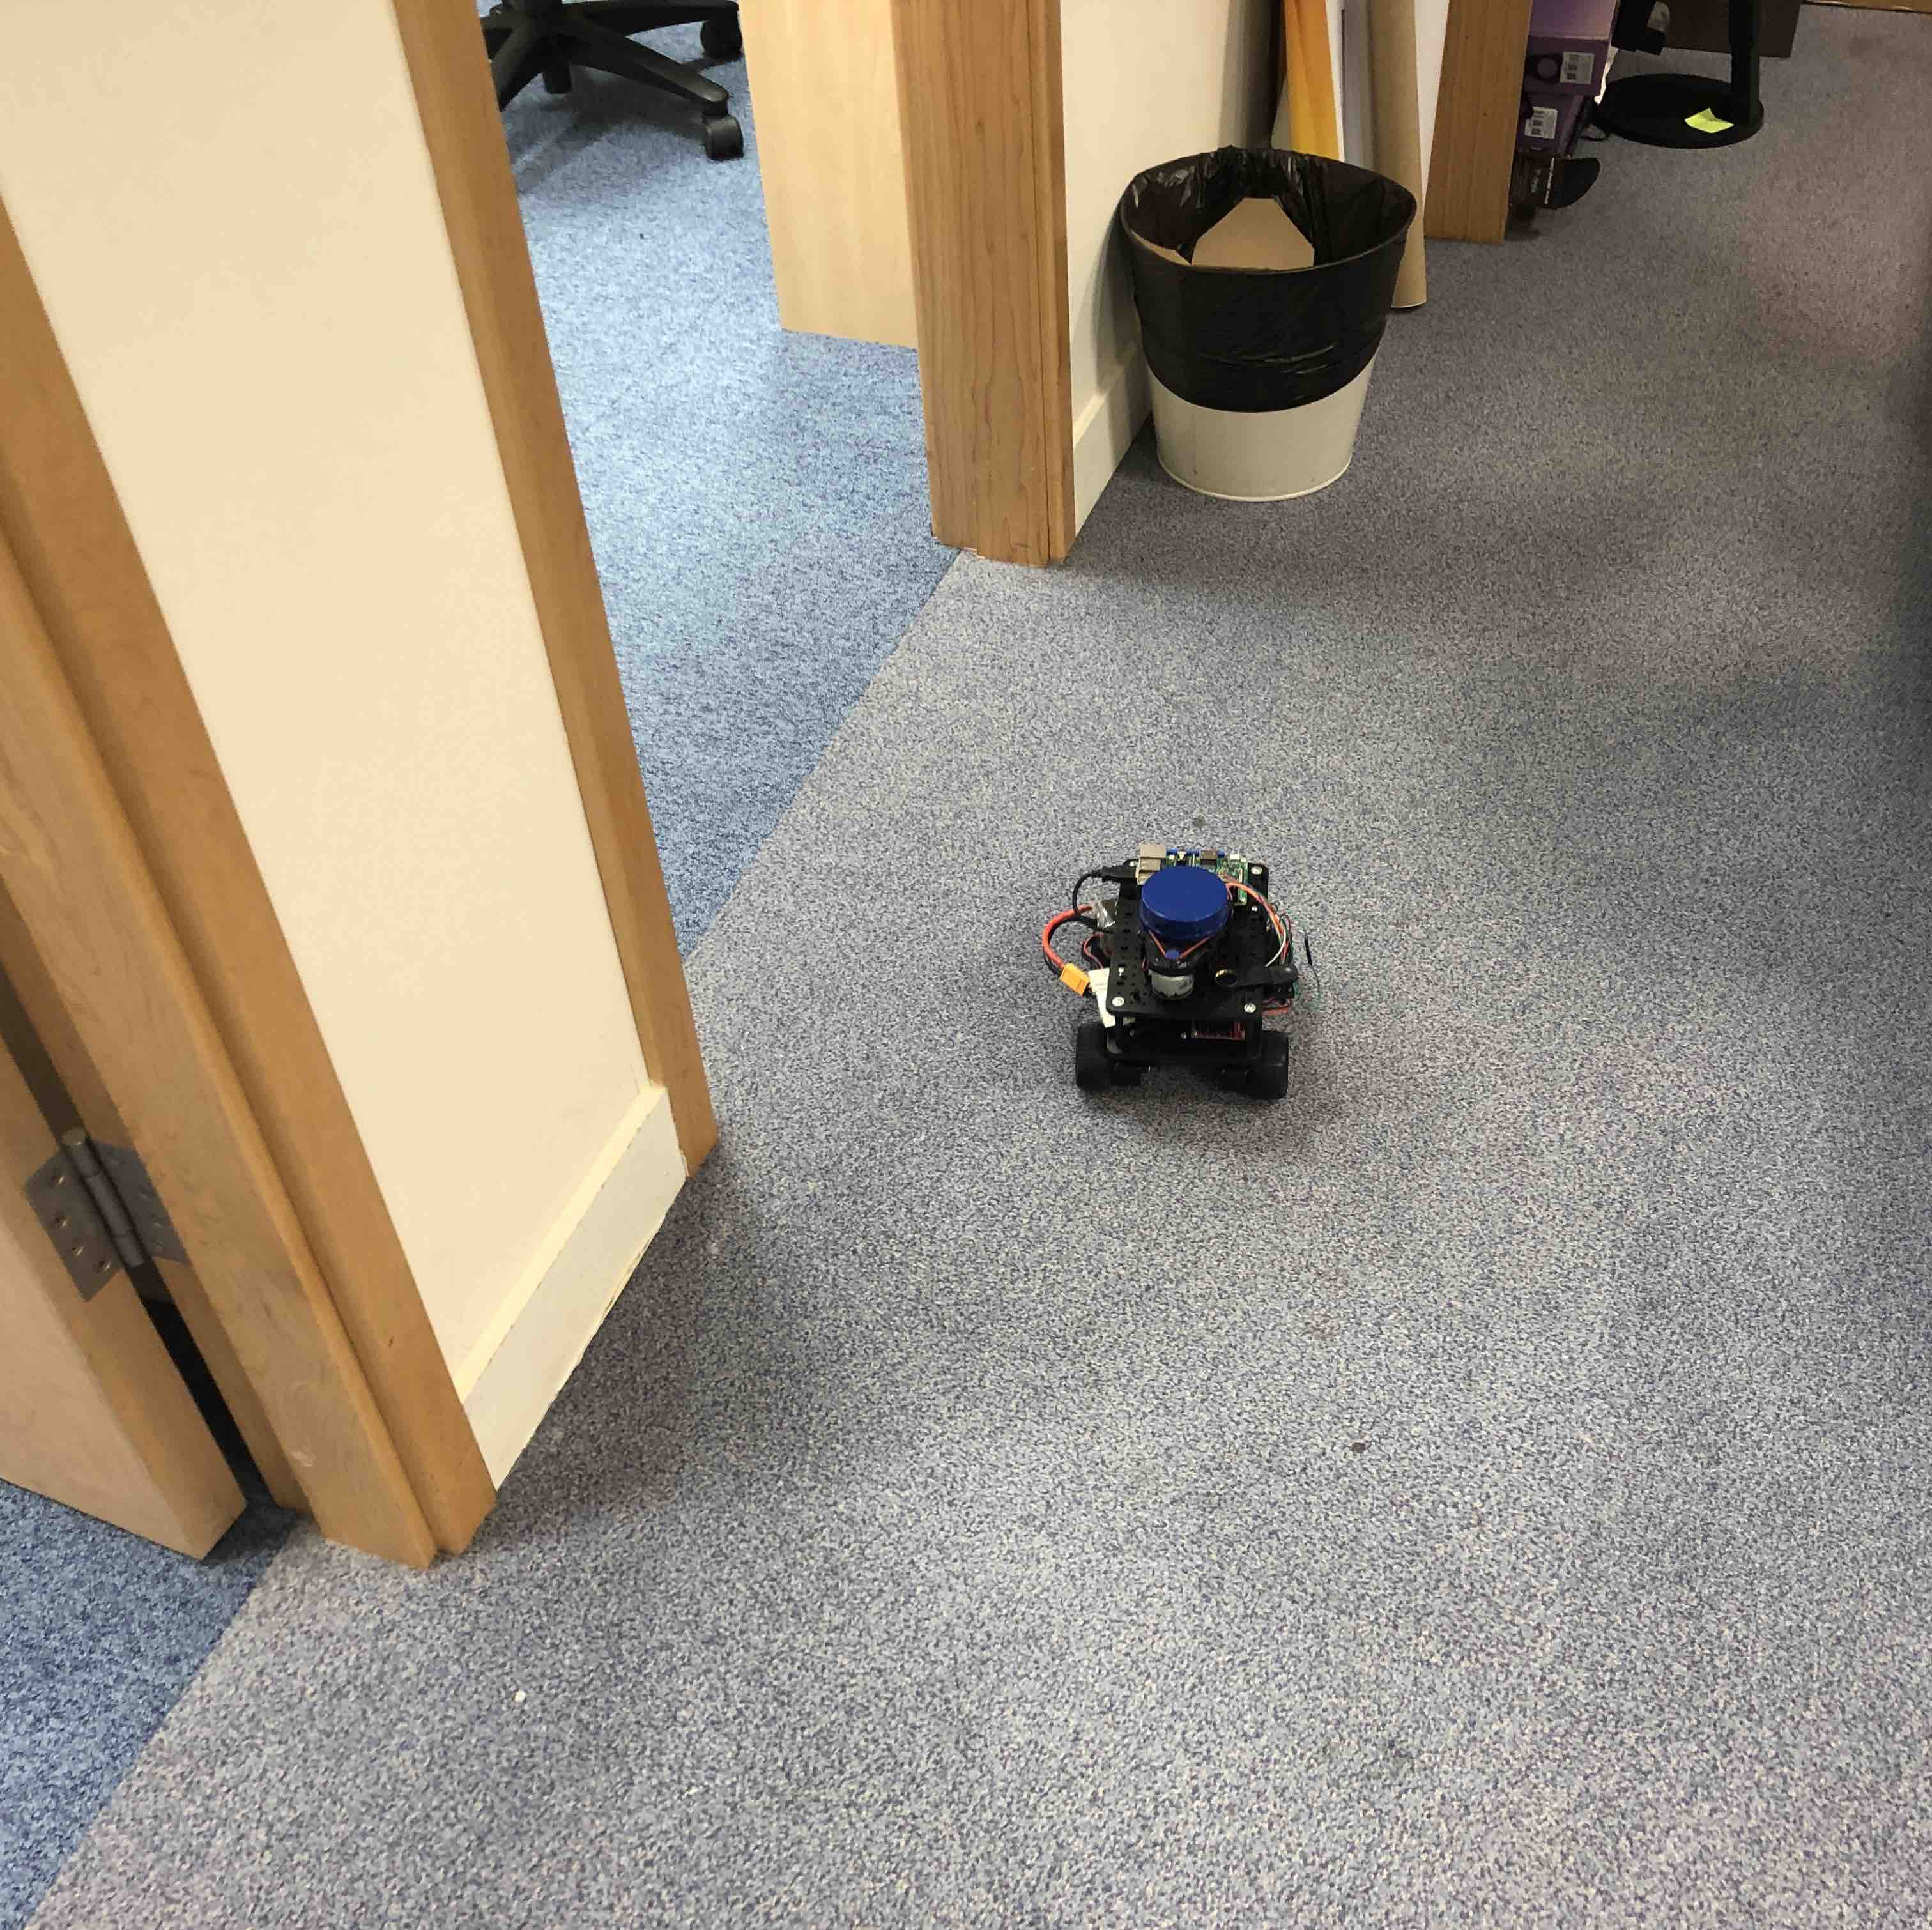
\includegraphics[width=\linewidth]{images/real/robo/3.JPG}
     \caption{Real-world: Suggested WP 2}
  \end{subfigure}
  \hfill
  \begin{subfigure}[b]{0.32\linewidth}
    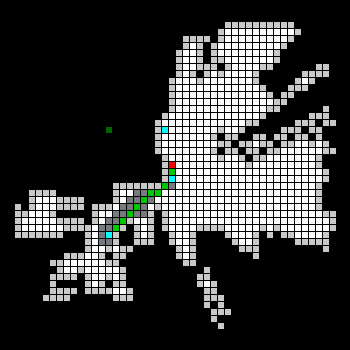
\includegraphics[width=\linewidth]{images/real/sys/3_2.png}
     \caption{PathBench: Suggested WP 2}
  \end{subfigure}
  \hfill
  \begin{subfigure}[b]{0.32\linewidth}
    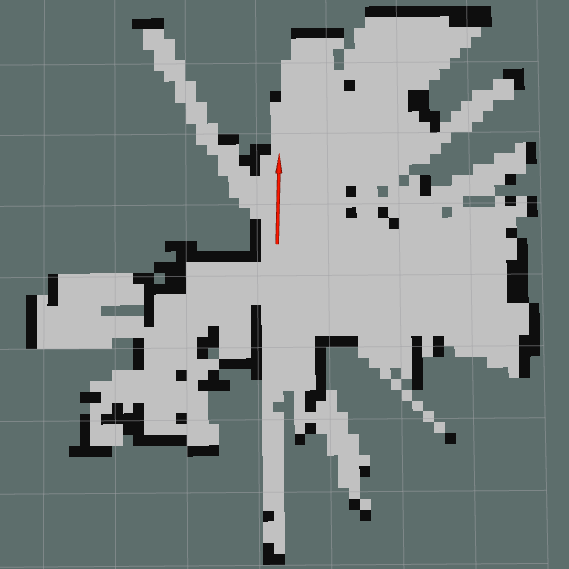
\includegraphics[width=\linewidth]{images/real/sys/3_3.png}
     \caption{Rviz: Suggested WP 2}
  \end{subfigure}
\end{figure}

\begin{figure}[htb]\ContinuedFloat
  \begin{subfigure}[b]{0.32\linewidth}
    \includegraphics[width=\linewidth]{images/real/robo/4.JPG}
     \caption{Real-world: Reached WP 2}
  \end{subfigure}
  \hfill
  \begin{subfigure}[b]{0.32\linewidth}
    \includegraphics[width=\linewidth]{images/real/sys/4_2.png}
     \caption{PathBench: Reached WP 2}
  \end{subfigure}
  \hfill
  \begin{subfigure}[b]{0.32\linewidth}
    \includegraphics[width=\linewidth]{images/real/sys/4_3.png}
     \caption{Rviz: Reached WP 2}
  \end{subfigure}
  
  \newline
  
  \begin{subfigure}[b]{0.32\linewidth}
    \includegraphics[width=\linewidth]{images/real/robo/5.JPG}
     \caption{Real-world: Suggested WP 3}
  \end{subfigure}
  \hfill
  \begin{subfigure}[b]{0.32\linewidth}
    \includegraphics[width=\linewidth]{images/real/sys/5_2.png}
     \caption{PathBench: Suggested WP 3}
  \end{subfigure}
  \hfill
  \begin{subfigure}[b]{0.32\linewidth}
    \includegraphics[width=\linewidth]{images/real/sys/5_3.png}
     \caption{Rviz: Suggested WP 3}
  \end{subfigure}
  
  \newline
  
  \begin{subfigure}[b]{0.32\linewidth}
    \includegraphics[width=\linewidth]{images/real/robo/final}
     \caption{Real-world: Final}
  \end{subfigure}
  \hfill
  \begin{subfigure}[b]{0.32\linewidth}
    \includegraphics[width=\linewidth]{images/real/sys/final_2.png}
     \caption{PathBench: Final}
  \end{subfigure}
  \hfill
  \begin{subfigure}[b]{0.32\linewidth}
    \includegraphics[width=\linewidth]{images/real/sys/final_3.png}
     \caption{Rviz: Final}
  \end{subfigure}
  
  \caption{Robot Path Planning using Global Way-point LSTM Planner run on the trajectory from Figure \ref{fig: robot}. The left image represents real-word view of the robot, the center image represents our live PathBench simulator visualisation and the right image represents the live Rviz simulator from ROS. The PathBench and Rviz images are cropped so that we only show the relevant information. The true dimension of the grid is $128 \times 128$}
  \label{fig: robot_run}
\end{figure}

\clearpage

\begin{table}[h!]
    \centering
    \begin{tabular}{|c|M{6.2cm}|}
         \hline
         \textbf{Name} & \textbf{Value} \\
         \hline
         Goal Found & \texttt{True} \\
         \hline
         Grid Cell Size & 0.15 meters \\
         \hline
         Map Size & $128 \times 128$ \\
         \hline
         Obstacles & 92.03\% \\
         \hline
         Original Distance & 15.00/2.25 meters \\
         \hline
         Distance & 28.56/4.824 meters \\
         \hline
         Time & 365.252545 seconds/6.08 minutes \\
         \hline
         Distance Left & 0.00/0.00 meters \\
         \hline
         Pick Ratio & [0.0\%, 33.33\%, 33.33\%, 0.0\%, 0.0\%, 33.33\%, 0.0\%, 0.0\%, 0.0\%, 0.0\%] \\
         \hline
         GK Improvement & 100.00\% \\
         \hline
         GK Distance & 28.56/4.824 meters \\
         \hline
         GK Distance Left & 0.00/0.00 meters \\
         \hline
         WP & \texttt{4} \\
         \hline
         WP In-Between Distance & 9.04/1.356 meters \\
         \hline
         Total Search & 0.47\% \\
         \hline
         Total Fringe & 0.31\% \\
         \hline
         Session Search & 0.13\% \\
         \hline
         Session Fringe & 0.09\% \\
         \hline
    \end{tabular}
    \caption{Reported real-world statistics on the run from Figure \ref{fig: robot_run}. The PathBench and Rviz images from Figure \ref{fig: robot_run} are cropped so that we only show the relevant information. The true dimension of the grid is $128 \times 128$}
    \label{tab: robot_stats}
\end{table}

The results show that the robot successfully found a path in a partial knowledge environment (See Figure \ref{fig: robot_run}) by placing the last global way-point on the goal. The evaluation metrics reported in Table \ref{tab: robot_stats} show that we retain the same behaviour discussed in the \textbf{Analyser} simple and complex routines (maximal GK Improvement, low number of way-points with high way-point in-between distance; it should be noted that time statistic is influenced by the speed of the robot). Therefore, we have shown that the Global Way-point LSTM Planner supports partial knowledge environments in which classic offline solutions such as A* are unable to find a path to the goal without making use of an exploration method. Lastly, we have showed that the simulator is compatible with the \textit{gmapping} \textit{ROS} package and has support for live updates.